% Arquivo LaTeX de exemplo de dissertação/tese a ser apresentada à CPG do IME-USP
%
% Criação: Jesús P. Mena-Chalco
% Revisão: Fabio Kon e Paulo Feofiloff
% Adaptação para UTF8, biblatex e outras melhorias: Nelson Lago
%
% Except where otherwise indicated, these files are distributed under
% the MIT Licence. The example text, which includes the tutorial and
% examples as well as the explanatory comments in the source, are
% available under the Creative Commons Attribution International
% Licence, v4.0 (CC-BY 4.0) - https://creativecommons.org/licenses/by/4.0/


%%%%%%%%%%%%%%%%%%%%%%%%%%%%%%%%%%%%%%%%%%%%%%%%%%%%%%%%%%%%%%%%%%%%%%%%%%%%%%%%
%%%%%%%%%%%%%%%%%%%%%%%%%%%%%%% PREÂMBULO LaTeX %%%%%%%%%%%%%%%%%%%%%%%%%%%%%%%%
%%%%%%%%%%%%%%%%%%%%%%%%%%%%%%%%%%%%%%%%%%%%%%%%%%%%%%%%%%%%%%%%%%%%%%%%%%%%%%%%

% A opção twoside (frente-e-verso) significa que a aparência das páginas pares
% e ímpares pode ser diferente. Por exemplo, as margens podem ser diferentes ou
% os números de página podem aparecer à direita ou à esquerda alternadamente.
% Mas nada impede que você crie um documento "só frente" e, ao imprimir, faça
% a impressão frente-e-verso.
%
% Aqui também definimos a língua padrão do documento (a última da lista) e
% línguas adicionais. Para teses do IME, no mínimo português e inglês são
% obrigatórios, porque independentemente da língua principal do texto é
% preciso fornecer o resumo nessas duas línguas. LaTeX aceita alguns nomes
% diferentes para a língua portuguesa; dentre as opções, prefira sempre
% "brazilian" para português brasileiro e "portuguese" para português europeu.
%\documentclass[a4paper,12pt,twoside,brazilian,english]{book}
\documentclass[a4paper,12pt,twoside,english,brazilian]{book}

% O preâmbulo de um documento LaTeX pode ser razoavelmente longo. Neste
% modelo, optamos por reduzi-lo, colocando praticamente tudo do preâmbulo
% nas packages "imegoodies" e "imelooks".
%
% imegoodies carrega diversas packages muito úteis e populares (algumas
% são praticamente obrigatórias, como amsmath, babel, array etc.). É
% uma boa ideia usá-la com outros documentos também. Ela inclui vários
% comentários explicativos e dicas de uso; não tenha medo de alterá-la
% conforme a necessidade.
%
% imelooks carrega algumas packages e configurações que definem a
% aparência do documento; você também pode querer usá-la (ou partes
% dela) com outros documentos para obter as mesmas fontes, margens
% etc. Tal como "imegoodies", pode valer a pena ler os comentários
% e fazer modificações nessa package. Com a opção "thesis", imelooks
% também define os comandos para capa, folha de rosto etc.
\usepackage{imegoodies}
\usepackage[thesis]{imelooks}
\usepackage{xcolor}

%\nocolorlinks % para impressão em P&B

% Diretórios onde estão as figuras; com isso, não é necessário (mas
% é permitido) colocar o caminho completo em \includegraphics. Note
% que a extensão nunca é necessária (mas é permitida), ou seja, o
% resultado é o mesmo com "\includegraphics{figuras/foto.jpeg}",
% "\includegraphics{foto.jpeg}", "\includegraphics{figuras/foto}"
% ou "\includegraphics{foto}".
\graphicspath{{figuras/},{fig/},{logos/},{img/},{images/},{imagens/}}

% Comandos rápidos para mudar de língua:
% \en -> muda para o inglês
% \br -> muda para o português
% \texten{blah} -> o texto "blah" é em inglês
% \textbr{blah} -> o texto "blah" é em português
\babeltags{br = brazilian, en = english}


%%%%%%%%%%%%%%%%%%%%%%%%%%%%%%%%%%%%%%%%%%%%%%%%%%%%%%%%%%%%%%%%%%%%%%%%%%%%%%%%
%%%%%%%%%%%%%%%%%%%%%%%%%%%%%%%%%% METADADOS %%%%%%%%%%%%%%%%%%%%%%%%%%%%%%%%%%%
%%%%%%%%%%%%%%%%%%%%%%%%%%%%%%%%%%%%%%%%%%%%%%%%%%%%%%%%%%%%%%%%%%%%%%%%%%%%%%%%

% O arquivo com os dados bibliográficos para biblatex; você pode usar
% este comando mais de uma vez para acrescentar múltiplos arquivos
\addbibresource{bibliografia.bib}

% Este comando permite acrescentar itens à lista de referências sem incluir
% uma referência de fato no texto (pode ser usado em qualquer lugar do texto)
%\nocite{bronevetsky02,schmidt03:MSc, FSF:GNU-GPL, CORBA:spec, MenaChalco08}
% Com este comando, todos os itens do arquivo .bib são incluídos na lista
% de referências
%\nocite{*}

% É possível definir como determinadas palavras podem (ou não) ser
% hifenizadas; no entanto, a hifenização automática geralmente funciona bem
\babelhyphenation{documentclass latexmk soft-ware clsguide} % todas as línguas
\babelhyphenation[brazilian]{Fu-la-no}
\babelhyphenation[english]{what-ever}

% Estes comandos definem o título e autoria do trabalho e devem sempre ser
% definidos, pois além de serem utilizados para criar a capa, também são
% armazenados nos metadados do PDF. O subtítulo é opcional.
\title{Árvores binárias de busca e a Conjectura da Otimalidade Dinâmica}
\translatedtitle{Binary search trees and the Dynamic Optimality Conjecture}

\author[masc]{Bruno Armond Braga}

\def\profa{Prof\kern.02em.\kern-.07emª\kern.07em}
\def\dra{Dr\kern-.04em.\kern-.11emª\kern.07em}

% Para TCCs, este comando define o supervisor
\orientador[fem]{\profa{} \dra{} Cristina Gomes Fernandes}

\banca{
  \profa{} \dra{} Fulana de Tal (orientadora) -- IME-USP [sem ponto final],
  % Em inglês, não há o "ª"
  %Prof. Dr. Fulana de Tal (advisor) -- IME-USP [sem ponto final],
  Prof. Dr. Ciclano de Tal -- IME-USP [sem ponto final],
  \profa{} \dra{} Convidada de Tal -- IMPA [sem ponto final],
}

% A página de rosto da versão para depósito (ou seja, a versão final
% antes da defesa) deve ser diferente da página de rosto da versão
% definitiva (ou seja, a versão final após a incorporação das sugestões
% da banca).
\tipotese{
  %mestrado,
  %doutorado,
  tcc,
  %definitiva, % É a versão para defesa ou a versão definitiva?
  %quali, % É qualificação?
  programa={Ciência da Computação},
}

\defesa{
  local={São Paulo},
  data=2024-08-10, % YYYY-MM-DD
}

% Se não houve bolsa, remova
%
% Norma sobre agradecimento por auxílios da FAPESP:
% https://fapesp.br/11789/referencia-ao-apoio-da-fapesp-em-todas-as-formas-de-divulgacao
%
% Norma sobre agradecimento por auxílios da CAPES (Portaria 206,
% de 4 de Setembro de 2018):
% https://www.in.gov.br/materia/-/asset_publisher/Kujrw0TZC2Mb/content/id/39729251/do1-2018-09-05-portaria-n-206-de-4-de-setembro-de-2018-39729135
%
%\apoio{O presente trabalho foi realizado com apoio da Coordenação
%      de Aperfeiçoamento\\ de Pessoal de Nível Superior -- Brasil
%      (CAPES) -- Código de Financiamento 001} % o código é sempre 001
%
%\apoio{This study was financed in part by the Coordenação de
%      Aperfeiçoamento\\ de Pessoal de Nível Superior -- Brasil
%      (CAPES) -- Finance Code 001} % o código é sempre 001
%
\apoio{Durante o desenvolvimento deste trabalho, o autor recebeu\\
      auxílio financeiro da FAPESP -- processo nº 2024/04708-2}
%
%\apoio{During the development if this work, the author received\\
%      financial support from FAPESP -- grant \#aaaa/nnnnn-d}
%\apoio{Durante o desenvolvimento deste trabalho o autor
%       recebeu auxílio financeiro da XXXX}

% A licença do seu trabalho. Use CC-BY, CC-BY-NC, CC-BY-ND, CC-BY-SA,
% CC-BY-NC-SA ou CC-BY-NC-ND para escolher a licença Creative Commons
% correspondente (o sistema insere automaticamente o texto da licença).
% Se quiser estabelecer regras diferentes para o uso de seu trabalho,
% converse com seu orientador e coloque o texto da licença aqui, mas
% observe que apenas TCCs sob alguma licença Creative Commons serão
% acrescentados ao BDTA. Se você tem alguma intenção de publicar o
% trabalho comercialmente no futuro, sugerimos a licença CC-BY-NC-ND.
%
%\direitos{CC-BY-NC-ND}
%
%\direitos{Autorizo a reprodução e divulgação total ou parcial deste
%          trabalho, por qualquer meio convencional ou eletrônico,
%          para fins de estudo e pesquisa, desde que citada a fonte.}
%
%\direitos{I authorize the complete or partial reproduction and disclosure
%          of this work by any conventional or electronic means for study
%          and research purposes, provided that the source is acknowledged.}
%
\direitos{CC-BY}

% Para gerar a ficha catalográfica, acesse https://fc.ime.usp.br/,
% preencha o formulário e escolha a opção "Gerar Código LaTeX".
% Basta copiar e colar o resultado aqui.
\fichacatalografica{}


%%%%%%%%%%%%%%%%%%%%%%%%%%%%%%%%%%%%%%%%%%%%%%%%%%%%%%%%%%%%%%%%%%%%%%%%%%%%%%%%
%%%%%%%%%%%%%%%%%%%%%%% AQUI COMEÇA O CONTEÚDO DE FATO %%%%%%%%%%%%%%%%%%%%%%%%%
%%%%%%%%%%%%%%%%%%%%%%%%%%%%%%%%%%%%%%%%%%%%%%%%%%%%%%%%%%%%%%%%%%%%%%%%%%%%%%%%

\newtheorem{theorem}{Teorema}[chapter]
\newtheorem{lemma}[theorem]{Lema}
\newcommand{\Oh}{\mathrm{O}}
%\newcommand{\Oh}{\mathcal{O}}


\begin{document}

%%%%%%%%%%%%%%%%%%%%%%%%%%% CAPA E PÁGINAS INICIAIS %%%%%%%%%%%%%%%%%%%%%%%%%%%%

% Aqui começa o conteúdo inicial que aparece antes do capítulo 1, ou seja,
% página de rosto, resumo, sumário etc. O comando frontmatter faz números
% de página aparecem em algarismos romanos ao invés de arábicos e
% desabilita a contagem de capítulos.
\frontmatter

\pagestyle{plain}

\onehalfspacing % Espaçamento 1,5 na capa e páginas iniciais

\maketitle % capa e folha de rosto

%%%%%%%%%%%%%%%% DEDICATÓRIA, AGRADECIMENTOS, RESUMO/ABSTRACT %%%%%%%%%%%%%%%%%%

%\begin{dedicatoria}
%Esta seção é opcional e fica numa página separada; ela pode ser usada para
%uma dedicatória ou epígrafe.
%\end{dedicatoria}

% Reinicia o contador de páginas (a próxima página recebe o número "i") para
% que a página da dedicatória não seja contada.
\pagenumbering{roman}

% Agradecimentos:
% Se o candidato não quer fazer agradecimentos, deve simplesmente eliminar
% esta página. A epígrafe, obviamente, é opcional; é possível colocar
% epígrafes em todos os capítulos. O comando "\chapter*" faz esta seção
% não ser incluída no sumário.
\chapter*{Agradecimentos}
\epigrafe{Do. Or do not. There is no try.}{Mestre Yoda}

Texto texto texto texto texto texto texto texto texto texto texto texto texto
texto texto texto texto texto texto texto texto texto texto texto texto texto
texto texto texto texto texto texto texto texto texto texto texto texto texto
texto texto texto texto. Texto opcional.

%!TeX root=../tese.tex
%("dica" para o editor de texto: este arquivo é parte de um documento maior)
% para saber mais: https://tex.stackexchange.com/q/78101

% As palavras-chave são obrigatórias, em português e em inglês, e devem ser
% definidas antes do resumo/abstract. Acrescente quantas forem necessárias.
\palavraschave{Palavra-chave1, Palavra-chave2, Palavra-chave3}

\keywords{Keyword1,Keyword2,Keyword3}

% O resumo é obrigatório, em português e inglês. Estes comandos também
% geram automaticamente a referência para o próprio documento, conforme
% as normas sugeridas da USP.
\resumo{
Elemento obrigatório, constituído de uma sequência de frases concisas e
objetivas, em forma de texto. Deve apresentar os objetivos, métodos empregados,
resultados e conclusões. O resumo deve ser redigido em parágrafo único, conter
no máximo 500 palavras e ser seguido dos termos representativos do conteúdo do
trabalho (palavras-chave). Deve ser precedido da referência do documento.
Texto texto texto texto texto texto texto texto texto texto texto texto texto
texto texto texto texto texto texto texto texto texto texto texto texto texto
texto texto texto texto texto texto texto texto texto texto texto texto texto
texto texto texto texto texto texto texto texto texto texto texto texto texto
texto texto texto texto texto texto texto texto texto texto texto texto texto
texto texto texto texto texto texto texto texto.
Texto texto texto texto texto texto texto texto texto texto texto texto texto
texto texto texto texto texto texto texto texto texto texto texto texto texto
texto texto texto texto texto texto texto texto texto texto texto texto texto
texto texto texto texto texto texto texto texto texto texto texto texto texto
texto texto.
}

\abstract{
Elemento obrigatório, elaborado com as mesmas características do resumo em
língua portuguesa. De acordo com o Regimento da Pós-Graduação da USP (Artigo
99), deve ser redigido em inglês para fins de divulgação. É uma boa ideia usar
o sítio \url{www.grammarly.com} na preparação de textos em inglês.
Text text text text text text text text text text text text text text text text
text text text text text text text text text text text text text text text text
text text text text text text text text text text text text text text text text
text text text text text text text text text text text text.
Text text text text text text text text text text text text text text text text
text text text text text text text text text text text text text text text text
text text text.
}



%%%%%%%%%%%%%%%%%%%%%%%%%%% LISTAS DE FIGURAS ETC. %%%%%%%%%%%%%%%%%%%%%%%%%%%%%

% Como as listas que se seguem podem não incluir uma quebra de página
% obrigatória, inserimos uma quebra manualmente aqui.
%\cleardoublepage

% Todas as listas são opcionais; Usando "\chapter*" elas não são incluídas
% no sumário. As listas geradas automaticamente também não são incluídas por
% conta das opções "notlot" e "notlof" que usamos para a package tocbibind.

% Normalmente, "\chapter*" faz o novo capítulo iniciar em uma nova página, e as
% listas geradas automaticamente também por padrão ficam em páginas separadas.
% Como cada uma destas listas é muito curta, não faz muito sentido fazer isso
% aqui, então usamos este comando para desabilitar essas quebras de página.
% Se você preferir, comente as linhas com esse comando e des-comente as linhas
% sem ele para criar as listas em páginas separadas. Observe que você também
% pode inserir quebras de página manualmente (com \clearpage, veja o exemplo
% mais abaixo).
%\newcommand\disablenewpage[1]{{\let\clearpage\par\let\cleardoublepage\par #1}}
\newcommand{\tdots}{{\,.\,.\,}}

% Nestas listas, é melhor usar "raggedbottom" (veja basics.tex). Colocamos
% a opção correspondente e as listas dentro de um grupo para ativar
% raggedbottom apenas temporariamente.
%\bgroup
%\raggedbottom

%%%%% Listas criadas manualmente

%\chapter*{Lista de abreviaturas}
%\disablenewpage{\chapter*{Lista de abreviaturas}}

%\begin{tabular}{rl}
%   CFT & Transformada contínua de Fourier (\emph{Continuous Fourier Transform})\\
%   DFT & Transformada discreta de Fourier (\emph{Discrete Fourier Transform})\\
%  EIIP & Potencial de interação elétron-íon (\emph{Electron-Ion Interaction Potentials})\\
%  STFT & Transformada de Fourier de tempo reduzido (\emph{Short-Time Fourier Transform})\\
%  ABNT & Associação Brasileira de Normas Técnicas\\
%   URL & Localizador Uniforme de Recursos (\emph{Uniform Resource Locator})\\
%   IME & Instituto de Matemática e Estatística\\
%   USP & Universidade de São Paulo
%\end{tabular}

%\chapter*{Lista de símbolos}
%\disablenewpage{\chapter*{Lista de símbolos}}

%\begin{tabular}{rl}
%  $\omega$ & Frequência angular\\
%    $\psi$ & Função de análise \emph{wavelet}\\
%    $\Psi$ & Transformada de Fourier de $\psi$\\
%\end{tabular}

% Quebra de página manual
%\clearpage

%%%%% Listas criadas automaticamente

% Você pode escolher se quer ou não permitir a quebra de página
%\listoffigures
%\disablenewpage{\listoffigures}

% Você pode escolher se quer ou não permitir a quebra de página
%\listoftables
%\disablenewpage{\listoftables}

% Esta lista é criada "automaticamente" pela package float quando
% definimos o novo tipo de float "program" (em utils.tex)
% Você pode escolher se quer ou não permitir a quebra de página
%\listof{program}{\programlistname}
%\disablenewpage{\listof{program}{\programlistname}}

% Sumário (obrigatório)
\tableofcontents

%\egroup % Final de "raggedbottom"

% Referências indiretas ("x", veja "y") para o índice remissivo (opcionais,
% pois o índice é opcional). É comum colocar esses itens no final do documento,
% junto com o comando \printindex, mas em alguns casos isso torna necessário
% executar texindy (ou makeindex) mais de uma vez, então colocar aqui é melhor.
%\index{Inglês|see{Língua estrangeira}}
%\index{Figuras|see{Floats}}
%\index{Tabelas|see{Floats}}
%\index{Código-fonte|see{Floats}}
%\index{Subcaptions|see{Subfiguras}}
%\index{Sublegendas|see{Subfiguras}}
%\index{Equações|see{Modo matemático}}
%\index{Fórmulas|see{Modo matemático}}
%\index{Rodapé, notas|see{Notas de rodapé}}
%\index{Captions|see{Legendas}}
%\index{Versão original|see{Tese/Dissertação, versões}}
%\index{Versão corrigida|see{Tese/Dissertação, versões}}
%\index{Palavras estrangeiras|see{Língua estrangeira}}
%\index{Floats!Algoritmo|see{Floats, ordem}}


%%%%%%%%%%%%%%%%%%%%%%%%%%%%%%%% CAPÍTULOS %%%%%%%%%%%%%%%%%%%%%%%%%%%%%%%%%%%%%

% Aqui vai o conteúdo principal do trabalho, ou seja, os capítulos que compõem
% a dissertação/tese. O comando mainmatter reinicia a contagem de páginas,
% modifica a numeração para números arábicos e ativa a contagem de capítulos.
\mainmatter

\pagestyle{mainmatter}

% Espaçamento simples
\singlespacing

% A introdução não tem número de capítulo, então os cabeçalhos também não
\pagestyle{unnumberedchapter}
%!TeX root=../tese.tex
%("dica" para o editor de texto: este arquivo é parte de um documento maior)
% para saber mais: https://tex.stackexchange.com/q/78101/183146

%% ------------------------------------------------------------------------- %%
\chapter{Introdução}
\label{cap:introducao}

Árvores Binárias de Busca (ABBs) são estruturas de dados que armazenam um conjunto de chaves de um universo estático, que possui uma ordem total, e dão suporte a buscas neste conjunto. Denotaremos por $n$ o número de elementos do conjunto armazenado na ABB considerada.

Estas estruturas são fundamentais na ciência da computação e possuem as mais diversas finalidades. Nesse projeto iremos estudar a chamada Conjectura da Otimalidade Dinâmica, interpretações geométricas de algoritmos de busca em ABBs e suas delimitações associadas. Também serão estudadas as árvores splay e as árvores tango.

Adaptando a definição dada por Sedgewick e Wayne \cite{Sedgewick}, \textit{árvore binária de busca} é uma árvore binária onde cada nó possui uma chave comparável e possivelmente um valor associado. Além disso, os nós satisfazem a restrição de que a chave em qualquer nó é maior do que as chaves em todos os nós na subárvore esquerda desse nó e menor do que as chaves em todos os nós na subárvore direita desse nó.

As ABBs também possuem um atributo \textit{raiz} que aponta para o nó raiz ou possui valor \textit{nulo}, caso a árvore esteja vazia.

\textit{Rotações} são operações que trocam dois nós, pai-filho, entre si enquanto mantém a restrição vista acima. Veja a Figura~\ref{fig:imagem}. Essa operação é fundamental para garantir performance em alguns algoritmos de ABBs e é muito utilizada para controlar a altura das árvores.


% Arrumar figura!!
\begin{figure}[h]
    \centering
    \includegraphics{imagens/zig2.pdf}
    \caption{Esquema de rotações.}
    \label{fig:imagem}
\end{figure}

No contexto da Conjectura da Otimalidade Dinâmica, apenas serão consideradas buscas bem sucedidas, que chamaremos de \textit{acessos}, e não são consideradas inserções ou remoções no conjunto armazenado. No modelo de computação adotado, um algoritmo de busca em uma ABB, para fazer o acesso a uma chave, mantém um único ponteiro. Chamamos de \textit{nó corrente} o nó apontado por esse ponteiro. 

No início da execução do acesso, o ponteiro aponta para a raiz da árvore e, após uma sequência de operações, deve encontrar o nó que armazena a chave procurada. As operações chamadas de \textit{primitivas} são:
\begin{enumerate}
    \item Mover o ponteiro para o filho esquerdo do nó corrente.
    \item Mover o ponteiro para o filho direito do nó corrente.
    \item Mover o ponteiro para o pai do nó corrente.
    \item Fazer uma rotação que troca a posição do nó corrente e do seu pai.
\end{enumerate}

O algoritmo tradicional de busca em ABB não executa a operação primitiva 4. Ele inicia a execução de um acesso na raiz e desce para o filho apropriado até alcançar a chave procurada. No modelo de computação adotado, todas essas operações possuem custo unitário.

Em geral, durante a execução de um acesso, uma série de nós distintos são apontados pelo ponteiro do algoritmo de busca. Ao fim da execução de uma busca bem sucedida, o nó corrente é o nó procurado. Assim, dizemos que o nó procurado foi \textit{acessado} e que todos os nós que foram apontados pelo ponteiro durante a busca foram \textit{visitados}. O nó acessado também é considerado um nó visitado.

O pior caso acontece quando a chave procurada está em um nó folha mais profundo. Nesse caso o algoritmo tem que passar por toda a altura da árvore até chegar a essa folha. Assim o custo do pior caso é proporcional à altura da árvore, que pode ser em princípio linear em $n$.

Com intuito de mitigar o custo do pior caso, algumas ABBs estrategicamente utilizam da operação primitiva 4 (rotação) para balancear o tamanho das subárvores e assim diminuir a altura da árvore. Um exemplo famoso, sobre o qual daremos mais detalhes à frente, é a árvore splay. Essa ABB executa rotações baseando-se na heurística ``move to front'' e assim balanceia a árvore durante as buscas. Essa árvore não utiliza armazenamento adicional para isso, ou seja, seus nós não têm campos extra.

O custo para executar um acesso nesse modelo está relacionado com o número de operações primitivas executadas até encontrar a chave procurada durante um acesso. 

No artigo de Demaine et al.~\cite{rotation_distance}, é demonstrada a seguinte propriedade sobre ABBs. É possível transformar qualquer ABB com $t$ nós em qualquer outra ABB com os mesmos $t$ nós com no máximo $2t - 6$ rotações. O número preciso não é tão relevante para a análise desse texto. O importante é notar que o número de rotações necessárias para transformar uma ABB $T$ com $t$ nós em uma ABB $T'$ com os mesmos $t$ nós disposta de qualquer outra maneira é $\Oh(t)$, ou seja, é linear no número de nós da ABB.

Por isso, podemos assumir que o número de rotações realizadas durante um acesso é linear no número de nós visitados, assim definiremos o custo para executar um acesso nesse modelo como o número de nós visitados durante esse acesso.

Como o conjunto armazenado nas ABBs que consideraremos não sofre alterações, podemos assumir que esse conjunto é \{1,2,\ldots,$n$\}.

ABBs \textit{online} são ABBs que apenas possuem informações sobre os acessos passados. Ou seja, se $X = (x_1, \ldots, x_m)$ é a sequência de acessos que serão feitos, onde cada $x_i \in \{1,2,\ldots,n\}$, ao acessar $x_{i}$, um algoritmo de busca online não tem conhecimento das chaves $x_{i+1},\ldots,x_{m}$, nem mesmo do valor de $m$. Em particular, muitas ABBs online possuem informações adicionais em cada nó que auxiliam o algoritmo de busca a decidir quando executar rotações durante a busca pelas chaves procuradas. Qualquer ABB online que usa $\Oh(1)$ palavras adicionais por nó possui tempo de execução dominado pelo número de operações primitivas.

Uma ABB é chamada de \textit{offline} se tem conhecimento da sequência $X$ de acessos antes de começar os acessos às chaves de $X$. Nesse contexto, o comportamento do algoritmo não depende unicamente do histórico de acessos passados, uma vez que o algoritmo possui conhecimento prévio de toda a sequência de chaves a serem acessadas.

Dada uma sequência $X$ de acessos, uma ABB é considerada \textit{ótima} se executa os acessos de $X$ com o menor custo possível. Podemos definir OPT$(X)$ como o número de nós visitados por uma ABB ótima para a sequência $X$. Em outras palavras, OPT$(X)$ é o número mínimo necessário de visitas a nós para uma ABB concluir todos os acessos de $X$. 

ABBs balanceadas estabelecem que OPT$(X)$ = $\Oh(m \log n)$, onde $n$ é o número de chaves armazenadas na árvore e $m$ é o comprimento de $X$. Como todo acesso tem custo maior ou igual a 1, então $\text{OPT}(X) \geq m$. Wilber \cite{lowerbound_wilber} provou que OPT$(X)$ = $\Theta$$(m \log n)$ para algumas classes de sequências $X$. 

% JÁ USEI ESSA FRASE!
Uma ABB online é \textit{dinamicamente ótima} se, para todas as sequências $X$, seu algoritmo de busca tem custo $\Oh$(OPT($X$)). De maneira mais geral, uma ABB online é \textit{$c$-competitiva} se executa todos os acessos da sequências $X$ suficientemente longas com custo no máximo $c$\,OPT($X$).

Todo esse estudo foi feito para tentar responder à pergunta: ``\textit{Existe uma ABB online dinamicamente ótima?}".

Uma das tentativas de responder tal pergunta foi a árvore splay de Sleator e Tarjan~\cite{selfadjustingbst}. Como já mencionamos, árvores splay são ABBs que seguem a heurística ``move to front". Mais precisamente, após cada acesso, a árvore se reestrutura de uma maneira particular, trazendo o nó da chave que foi acessada para a raiz da árvore.

Apesar de existirem muitas ABBs muito bem documentadas com tempo por busca logarítmico em $n$, essas estruturas normalmente não conseguem alcançar uma eficiência superior a isso independentemente da entrada. Padrões de acesso do mundo real muitas vezes possuem estruturas repetitivas, como por exemplo bancos de dados que recebem solicitações frequentes para um pequeno número de elementos de alto tráfego. Em alguns desses casos, é possível ter uma performance melhor que $\Theta(\log n)$ por acesso utilizando uma árvore splay, uma vez que essa eventualmente ficaria com as chaves mais acessadas mais próximas à raiz da árvore. 

Há uma conjectura não resolvida no artigo \cite{selfadjustingbst} que diz que as árvores splay são dinamicamente ótimas. Essa conjectura ficou conhecida como a Conjectura da Otimalidade Dinâmica.

A árvore conhecida que mais se aproxima de uma árvore ótima é a árvores tango~\cite{dynamicoptimality}. Tal estrutura é $\Oh(\lg \lg n)$-competitiva. Esta árvore, proposta por Demaine, Harmon, Iacono e Pătrașcu \cite{dynamicoptimality}, utiliza $\Oh(\lg \lg n)$ bits a mais por nó e o custo para determinar a próxima operação primitiva a ser executada é amortizadamente constante.

%Nas árvores tango, há a definição de \textit{filho preferido}. O \textit{filho preferido} de um nó é o filho direito se ele foi o nó mais recentemente acessado em comparação com o nó esquerdo, e caso contrário (incluindo o caso em que nenhum dos dois filhos foi acessado ainda), definimos o nó esquerdo como \textit{filho preferido}.

%Define-se então um \textit{caminho preferido} como um caminho maximal de um nó da ABB até a folha que passa apenas por \textit{filhos preferidos}. 

%Os caminhos preferidos particionam os nós da árvore. Nas árvores tango, os nós de cada caminho preferido são armazenados em uma ABB balanceada tendo como chave a profundidade do nó no caminho. Essas árvores auxiliares estão interligadas de uma maneira apropriada.

%Durante os \textit{acessos}, os \textit{filhos preferidos} podem ser alterados e isso provocará mudanças nas estruturas da árvores auxiliares para manter a estrutura da árvore tango coerentes com o comportamento descrito acima.

Nesse texto, abordaremos uma série de aspectos diferentes em relação a delimitações de custo em algoritmos de busca em ABBs e implementações visando o menor custo possível. No Capítulo 2, será discutido o problema de encontrar uma ABB estática de custo mínimo para uma determinada sequência de acessos. No Capítulo 3, abordaremos o funcionamento e o custo das operações das árvores splay e apresentaremos a Conjectura da Otimalidade Dinâmica. 
No Capítulo 4, examinaremos como tratar buscas em ABBs de maneira geométrica por meio de conjuntos arboreamente satisfeitos e será proposto um algoritmo offline guloso para encontrar conjuntos arboreamente satisfeitos para sequências de entradas. %e será apresentada uma análise de como transforma-lo em um algoritmo online. 
No Capítulo 5, ampliaremos a análise geométrica para desenvolver uma nova delimitação relacionada a retângulos independentes. O Capítulo 6 tratará das delimitações de Wilber e, por fim, no Capítulo 7 explicaremos como funcionam as árvores tango.
\pagestyle{mainmatter}
%!TeX root=../tese.tex
%("dica" para o editor de texto: este arquivo é parte de um documento maior)
% para saber mais: https://tex.stackexchange.com/q/78101/183146

%% ------------------------------------------------------------------------- %%
\chapter{Problema Estático}
\label{cap:problema-estatico}

Neste capítulo será apresentado a solução para encontrar uma árvore de busca binária com custo mínimo para um determinado 
%!TeX root=../tese.tex
%("dica" para o editor de texto: este arquivo é parte de um documento maior)
% para saber mais: https://tex.stackexchange.com/q/78101/183146

%% ------------------------------------------------------------------------- %%
\chapter{Árvores splay}
\label{cap:arvores-splay}

Neste capítulo apresentaremos a estrutura Árvore Splay desenvolvida por \cite{selfadjustingbst}. Descreveremos a implementação e funcionamento das operações splay, acess, insert, delete, split e join e analisaremos o custo amortizado da árvore.


\section{Introdução}
O algoritmo tradicional de busca em ABB inicia a execução de um acesso na raiz e desce para o filho apropriado até alcançar a chave procurada. O pior caso é quando a chave procurada está em um nó folha mais profundo. Nesse caso, o algoritmo tem que passar por toda a altura da árvore até chegar a essa folha. Assim o custo do pior caso é proporcional à altura da árvore que, no pior dos casos é linear $\mathcal{O}(n)$ e no melhor dos casos, tem custo $\mathcal{O}(\log{}n)$.

Com base neste limitante inferior de custo $\Omega(\log{}n)$ para buscas em ABBs, foram desenvolvidas uma série de estruturas conhecidas como \textit{árvores binárias de busca balanceadas}. Essas árvores têm o intuito de minimizar a própria altura por meio de rotações e consequentemente mitigar o custo de acessos de pior caso. Muitas dessas estruturas também se utilizam de armazenamento de memória adicional por nó para manter informações essenciais para a lógica de balanceamento proposta. 

Apesar dessas estruturas serem bastante eficientes, tendo tempo por busca logarítmico no número de elementos, elas não conseguem alcançar uma eficiência superior a isso independente da entrada. Padrões de acesso do mundo real muitas vezes possuem tendências ou estruturas repetitivas, como por exemplo bancos de dados que recebem solicitações frequentes para um pequeno número de elementos de alto tráfego. Em alguns desses casos, é possível ter uma performance melhor que $\mathcal{O}(\log{}n)$ mesmo com um algoritmo de busca online.

Uma alternativa para uma performance melhor é a árvore splay. Árvore Splay é uma árvore binária de busca balanceada proposta por \cite{selfadjustingbst}. Diferentemente das árvores binárias balanceadas citadas anteriormente, a árvore splay se reestrutura após cada operação, inclusive após acessos e não utiliza armazenamento adicional.

A árvore splay é uma ABB que segue a heurística “move to front”, ou seja, a ideia central é que a medida que operações são realizadas na estrutura, os elementos são movidos para perto da raiz de uma maneira particular com intuito de manter na raiz o último nó acessado.
Com a tendência dos nós mais recentemente acessados estarem próximos da raiz, o custo de sequências de acessos repetitivos tende a diminuir e essas reestruturações também auxiliam a árvore splay a dispor seus nós de maneira mais balanceada, reduzindo a altura total da árvore em alguns casos.

\section{Operação Splay}

A essência da árvore splay está na operação splay A operação splay é a responsável por mover um nó específico para a raiz por meio de rotações sucessivas. Essa operação é fundamental para o funcionamento da estrutura e é utilizada por todas as outras operações.

A operação splay se utiliza de três tipos distintos de rotações para trazer um nó para a raiz: zig, zig-zig e zig-zag.

Seja $x$ o nó interno a ser deslocado para a raiz. 

\subsection{Caso zig}

A rotação zig acontece quando $x$ é descendente direto do nó raiz. Neste caso apenas é necessário realizar uma rotação no nó $x$ e $x$ se encontrará na raiz da árvore.

\begin{figure}[h]
    \centering
    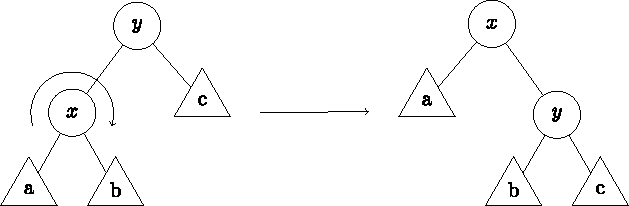
\includegraphics{images/zig.pdf}
    \label{fig:zig}

\caption{Caso zig com $x$ nó esquerdo da raiz.}
\end{figure}

\subsection{Caso zig-zig}

A rotação zig-zig acontece quando $x$ e seu pai são ambos filhos direitos ou ambos filhos esquerdos. Neste caso, é necessário rotacionar o pai de $x$ primeiro e em seguida rotacionar $x$.

\begin{figure}[h]
    \centering
    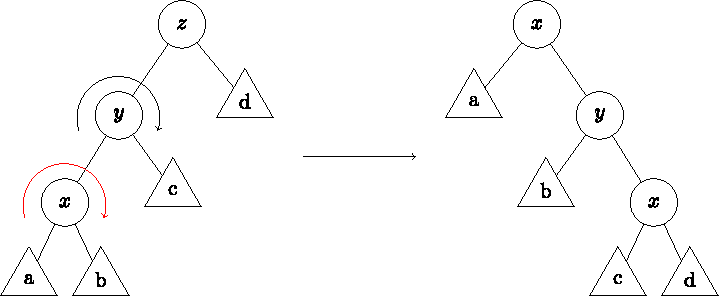
\includegraphics{images/zigzig.pdf}
    \label{fig:zigzig}

\caption{Caso zig-zig com $x$ e $y$ filhos esquerdos. A flecha preta e a vermelha representam respectivamente as rotações a serem realizadas em primeiro e por último.}
\end{figure}

\subsection{Caso zig-zag}

A rotação zig-zag acontece quando $x$ e seu pai não são ambos filhos direitos ou ambos filhos esquerdos. Neste caso, é necessário rotacionar $x$ duas vezes. Vale ressaltar que cada rotação será feita para um lado.
%\begin{figure}[hbt!]
%\centering
%\begin{tikzpicture}[
%ed/.style = {densely dashed, shorten >= 5pt},
%alpha/.style = {regular polygon, regular polygon sides=3, draw, minimum size=1.1cm, inner sep=2pt, anchor=south},
%level distance=1.5cm,
%sibling distance=0.25cm 
%]
%\begin{scope}[local bounding box=scope1]
%    \Tree [.$z$  [.$y$ \node[alpha]{a}; [.$x$ \node[alpha]{b}; \node[alpha]{c}; ]] \node[alpha]{d};]
%\end{scope}

%\begin{scope}[xshift=6cm, local bounding box=scope2, scale=1, level distance=2.25cm, sibling distance=0.25cm]
%    \Tree [.$x$ [.$y$ \node[alpha]{a}; \node[alpha]{b};] [.$z$  \node[alpha]{c}; \node[alpha]{d};]]]
%\end{scope}

%\draw[->] ([yshift=-0.5*\ht\strutbox,xshift=0.5cm]scope1.east) -- node {} ([yshift=-0.5*\ht\strutbox,xshift=-0.1cm]scope2.west); 

%\draw[->] ([yshift=-3.67cm, xshift=0.67cm]scope1.north) arc (-18:198:0.7cm);
%\draw[->,red] ([yshift=-3.67cm, xshift=-0.78cm]scope1.north) arc (198:-18:0.82cm);

%\end{tikzpicture}

\begin{figure}[h]
    \centering
    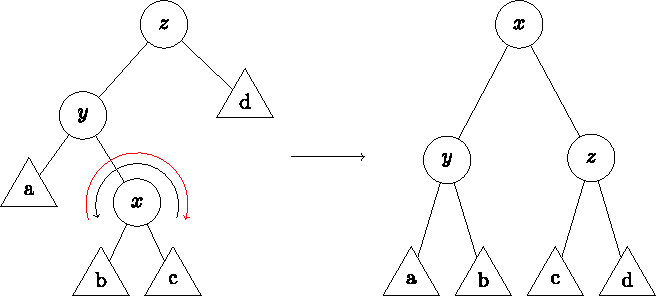
\includegraphics{images/zigzag.pdf}
    \label{fig:zigzag}

\caption{Caso zig-zag com $x$ filho direito e $y$ filho esquerdo. A flecha preta e a vermelha representam respectivamente as rotações a serem realizadas em primeiro e por último.}
\end{figure}

%!TeX root=../tese.tex
%("dica" para o editor de texto: este arquivo é parte de um documento maior)
% para saber mais: https://tex.stackexchange.com/q/78101/183146

%% ------------------------------------------------------------------------- %%
\chapter{Interpretação geométrica de buscas em ABBs}
\label{cap:geometria}

Neste capítulo explicaremos a visão geométrica proposta por Demaine, Harmon, Iacono e Pătrașcu \cite{geometry_of_bst}, o que são conjuntos de pontos arboreamente satisfeitos e como interpretar de maneira geométrica algoritmos de busca em ABBs.

\section{Conjuntos arboreamente satisfeitos}

Chamamos dois pontos $a$ e $b$ de \textit{ortogonalmente colineares} se $a$ e $b$ estão na mesma linha horizontal ou vertical. Se $a$ e $b$ não são ortogonalmente colineares, denotamos por \textit{$\{a,b\}$-retângulo} o retângulo ortogonal que tem $a$ e $b$ como vértices.

Um par de pontos $\{a,b\}$ de um conjunto de pontos $P$ é \textit{arboreamente satisfeito} se $a$ e $b$ são ortogonalmente colineares ou se há pelo menos um ponto do conjunto \( P \setminus \{a,b\} \) que está dentro da região delimitada pelo \{a,b\}-retângulo, incluindo seu perímetro. Um conjunto $P$ de pontos é \textit{arboreamente satisfeito} se todos os pares de pontos do conjunto são arboreamente satisfeitos. Veja a Figura~\ref{fig:geometria-inicial}.

\begin{figure}[h!]
    \centering
    \begin{minipage}[b]{0.45\textwidth}
        \centering
        \begin{tikzpicture}[scale=0.8]
        \begin{axis}[
            grid=major,
            xmin=0, xmax=4,
            ymin=0, ymax=4,
            xtick={0,1,2,3,4},
            ytick={0,1,2,3,4}
        ]
        \addplot[only marks, mark=*, mark size=3pt] coordinates {
            (1,1)
            (1,2)
            (1,3)
            (2,2)
            (2,3)
            (3,2)
        };
        \end{axis}
        \end{tikzpicture}
    \end{minipage}\hfill
    \begin{minipage}[b]{0.45\textwidth}
        \centering
        \begin{tikzpicture}[scale=0.8]
        \begin{axis}[
            grid=major,
            xmin=0, xmax=4,
            ymin=0, ymax=4,
            xtick={0,1,2,3,4},
            ytick={0,1,2,3,4}
        ]
        \addplot[only marks, mark=*, mark size=3pt] coordinates {
            (1,1)
            (1,2)
            (2,1)
            (3,3)
        };
        \addplot[
            color=red,
            line width=1.5pt
        ]
        coordinates {
            (2,1)
            (3,1)
            (3,3)
            (2,3)
            (2,1)
        };
        \addplot[
            color=red,
            line width=1.5pt
        ]
        coordinates {
            (1,2)
            (3,2)
            (3,3)
            (1,3)
            (1,2)
        };
        \end{axis}
        \end{tikzpicture}
    \end{minipage}
    \caption{À esquerda, um conjunto $P$ de pontos arboreamente satisfeito. À direita, um conjunto $P$ de pontos com dois pares de pontos arboreamente insatisfeitos com seus retângulos destacados.}
\label{fig:geometria-inicial}
\end{figure}

\begin{lemma}
\label{lem:pontos_em_arestas_incidentes}
Em um conjunto arboreamente satisfeito $P$, para todo par de pontos $\{a,b\}$ não ortogonalmente colineares, há sempre pelo menos um ponto de \( P \setminus \{a,b\} \) que está em um dos lados do $\{a,b\}$-retângulo que incide em $a$, e há sempre também pelo menos um ponto de \( P \setminus \{a,b\} \) que está em um dos lados do $\{a,b\}$-retângulo que incide em $b$.
\end{lemma}

\begin{figure}
    \begin{tikzpicture}[scale=1.5]
        \draw[blue, thick] (0,0) rectangle (2,1);
        
        \node at (0,0) [below left] {$a$};
        \node at (2,1) [above right] {$b$};
        
        \draw[red, thick] (0,0) -- (0,1);
        \draw[red, thick] (0,0) -- (2,0);
        \draw[blue, thick] (2,1) -- (0,1);
        \draw[blue, thick] (2,1) -- (2,0);
    \end{tikzpicture}
    \caption{O $\{a,b\}$-retângulo. Em vermelho estão destacados os lados do retângulo que incidem em $a$ e em azul estão destacados os lados que incidem em $b$.}
\end{figure}

\begin{proof}
    %Provaremos essa propriedade a partir de uma indução no número de pontos no interior dos retângulos. Seja $P$ o conjunto de pontos arboreamente satisfeito sendo analisado e sejam $a$ e $b$ dois pontos de $P$.
    %O caso base da indução é quando não há pontos de $P$ no interior do $\{a,b\}$-retângulo. Se existir algum ponto de $P \setminus \{a,b\}$ em um dos vértices do $\{a,b\}$-retângulo, então a propriedade é valida. Caso contrário, é necessário analisar as arestas do $\{a,b\}$-retângulo. Assuma sem perda de generalidade que $b$ está acima e a direita de $a$. 
    %Denotemos por $c$ o ponto de $P$ mais a esquerda na aresta horizontal superior. Denotemos por $d$ o ponto de $P$ mais abaixo na aresta vertical direita.
    %Se $c$ for diferente de $b$, então obrigatoriamente existe um ponto de $P$ com mesma coordenada $x$ de $c$ na aresta horizontal inferior, pois, caso contrário, $c$ e o ponto com maior coordenada $x$ na aresta horizontal inferior que possua coordenada $x$ menor que $c$ formariam um par de pontos arboreamente insatisfeito.
    %Se $c$ for igual a $b$, então obrigatoriamente $d$ é diferente de $b$, e pelo mesmo argumento geométrico, deve existir um ponto de $P$ com mesma coordenada $y$ na aresta vertical esquerda, pois caso contrário, o ponto $d$ e o ponto com maior coordenada $y$ na aresta vertical esquerda que possua coordenada $y$ menor que $d$ formariam um par de pontos arboreamente insatisfeito.

    Vamos provar por indução em $k$ que, todo $\{a,b\}$-retângulo com $k$ pontos em seu interior satisfaz a propriedade do Lema.

    Para $k = 0$, todo $\{a,b\}$-retângulo possui um ponto de $P \setminus \{a,b\}$ em um de seus vértices ou possui dois pontos de $P \setminus \{a,b\}$ em seu perímetro alinhados verticalmente ou horizontalmente. Caso o $\{a,b\}$-retângulo possua um ponto de $P \setminus \{a,b\}$ em um de seus vértices, então a propriedade é válida. Caso o $\{a,b\}$-retângulo possua dois pontos de $P \setminus \{a,b\}$ em seu perímetro alinhados verticalmente ou horizontalmente, então um desses pontos está em um dos lados do $\{a,b\}$-retângulo que incide em $a$ e o outro está em um dos lados do $\{a,b\}$-retângulo que incide em $b$, satisfazendo a propriedade do lema.

    Suponha agora que $k > 0$ e que a propriedade vale para todo retângulo com menos que $k$ pontos de $P$ em seu interior. Seja $e$ um ponto de $P$ no interior do $\{a,b\}$-retângulo. O $\{a,e\}$-retângulo e o $\{e,b\}$-retângulo são retângulos de $P$ com menos que $k$ pontos, logo a propriedade vale para esses retângulos. Como os lados do $\{a,b\}$-retângulo que incidem em $a$ contém os lados do $\{a,e\}$-retângulo que incidem $a$ e os lados do $\{a,b\}$-retângulo que incidem em $b$ contém os lados do $\{e,b\}$-retângulo que incidem $b$, então a propriedade vale também para o $\{a,b\}$-retângulo.
\end{proof}

\section{Visão geométrica de buscas}

No modelo de computação adotado, para realizar um acesso em uma ABB, o algoritmo de busca inicia o nó corrente na raiz da ABB. Em seguida, percorre a árvore descendo para o filho apropriado por meio de comparações até alcançar a chave procurada.

Dada uma sequência $X = (x_{1},\ldots,x_{m})$ de $m$ acessos às chaves $1,2,\ldots,n$, é possível ilustrar essa sequência $X$ de maneira gráfica em um plano cartesiano da seguinte forma: o eixo $x$ representará as chaves armazenadas na ABB e o eixo $y$ representará os índices $i = 1,2,\ldots,m$, que interpretamos como o tempo. Denotaremos por $P_X$ esse conjunto de pontos que chamaremos de \textit{visão geométrica da sequência de acessos}. Assim, um ponto de coordenada ($x$,$i$) representa a busca da chave $x$ na ABB no instante de tempo $i$, ou seja, representa $x_i$. Veja o exemplo da Figura~\ref{fig:busca_padrao}.

\begin{figure}
    \begin{tikzpicture}[scale=0.67]
        \begin{axis}[
            xlabel={Chaves},
            ylabel={Buscas},
            xlabel style={font=\large},
            ylabel style={font=\large},
            grid=major,
            xmin=0, xmax=11,
            ymin=0, ymax=11,
            xtick={0,2,4,6,8,10},
            ytick={0,2,4,6,8,10}
        ]
        \addplot[only marks, mark=*, mark size=2.5pt] coordinates {
            (1,9)
            (2,2)
            (3,6)
            (4,10)
            (5,8)
            (6,4)
            (7,1)
            (8,7)
            (9,3)
            (10,5)
        };
        \end{axis}
    \end{tikzpicture}
    \caption{Gráfico representando a sequência (7, 2, 9, 6, 10, 3, 8, 5, 1, 4) de acessos.}
\label{fig:busca_padrao}
\end{figure}

A \textit{visão geométrica da execução de um algoritmo de busca em ABB} para uma sequência $X = (x_{1},\ldots,x_{m})$ de buscas, de maneira similar, é o conjunto $P$ de pontos na forma ($x$,$i$) tal que $x$ é a chave de um dos nós visitados durante a busca pela chave $x_i$. Para cada $i \in \{1,\ldots,m\}$, os pontos de $P$ pertencentes a reta $y = i$ representam as chaves dos nós visitados durante a busca por $x_i$. Veja a Figura~\ref{fig:traducao-busca-em-ASS}.

\begin{figure}[h!]
    \centering
    \begin{minipage}[b]{0.34\textwidth}
        \centering
        \begin{tikzpicture}[scale=0.6]
        \begin{axis}[
            grid=major,
            xmin=0, xmax=6,
            ymin=0, ymax=6,
            xtick={1,2,3,4,5},
            ytick={1,2,3,4,5}
        ]
        \addplot[only marks, mark=*, mark size=3pt] coordinates {
            (3,1)
            (1,2)
            (4,3)
            (2,4)
            (5,5)
        };
        \end{axis}
        \end{tikzpicture}
    \end{minipage}\hfill
    \begin{minipage}[b]{0.33\textwidth}
        \centering
        \begin{tikzpicture}
            [node/.style={circle,draw,minimum size=1.5em}]
            \node[node] (A) at (-1.5,-1.5) {$1$};
            \node[node] (B) at (0,0) {$2$};
            \node[node] (C) at (0.5,-3) {$3$};
            \node[node] (D) at (1.5,-1.5) {$4$};
            \node[node] (E) at (2.5,-3) {$5$};
            
            \draw (A) -- (B);
            \draw (B) -- (D);
            \draw (C) -- (D);
            \draw (E) -- (D);
          \end{tikzpicture}
    \end{minipage}\hfill
    \begin{minipage}[b]{0.33\textwidth}
        \centering
        \begin{tikzpicture}[scale=0.6]
            \begin{axis}[
                grid=major,
                xmin=0, xmax=6,
                ymin=0, ymax=6,
                xtick={1,2,3,4,5},
                ytick={1,2,3,4,5}
            ]
            \addplot[only marks, mark=*, mark size=3pt] coordinates {
                (3,1)
                (1,2)
                (4,3)
                (2,4)
                (5,5)
            };
            \addplot[color=red, only marks, mark=*, mark size=3pt] coordinates {
                (2,1)
                (4,1)
                (2,2)
                (2,3)
                (2,5)
                (4,5)
            };
            \end{axis}
            \end{tikzpicture}
    \end{minipage}
    \caption{À esquerda, o conjunto de pontos que representa a sequência $X = (3,1,4,2,5)$. No meio, uma possível ABB com as chaves \{1,2,\ldots,5\}. À direita, a visão geométrica do algoritmo de busca que não efetua rotações na ABB do meio. Os pontos pretos são pontos de $P_X$ relacionados à sequência de acessos e os pontos vermelhos são o restante dos nós visitados durante cada um desses acessos. Note que o conjunto de pontos à esquerda não é arboreamente satisfeito, mas o conjunto à direita é.}
\label{fig:traducao-busca-em-ASS}
\end{figure}

\begin{lemma} A visão geométrica de qualquer execução de um algoritmo de busca em ABB no modelo de computação adotado é um conjunto de pontos arboreamente satisfeito.
\label{lema:visao_geometrica_vira_ASS}
\end{lemma}

\begin{proof}
Seja $P$ a visão geométrica da execução de um algoritmo de busca em uma ABB $T$ para alguma sequência $X$ de buscas.
Suponha, por contradição, que $P$ não é um conjunto arboreamente satisfeito. Dessa maneira, há pelo menos um par $\{p,q\}$ de pontos de $P$ que não é arboreamente satisfeito, onde $p = (a,i)$ e $q = (b,j)$. Assumiremos sem perda de generalidade que $i < j$ e $a < b$.

Seja $r$ o nó de $T$ com chave $a$ e seja $s$ o nó de $T$ com chave $b$.

Dois lados do $\{p,q\}$-retângulo terão um papel a seguir na prova. São eles:
\begin{itemize}
    \item $\ell_1$ = \{$(x,y)$ | $a \leq x < b$ e $y = j$\}, e
    \item $\ell_2$ = \{$(x,y)$ | $x = b$ e $i \leq y < j$\},
\end{itemize}
onde, dentro do contexto da ABB $T$, $\ell_1$ representa as visitas aos nós com chave no intervalo $[a,b)$ no instante $j$ e $\ell_2$ representa as visitas ao nó $s$ entre os instantes de tempo $i$ e $j$.

Como $\{p,q\}$ é um par de pontos arboreamente insatisfeito, nota-se que não há nenhum ponto de $P$ tanto nas bordas quanto no interior do $\{p,q\}$-retângulo. Logo, $(\ell_1 \cup \ell_2) \cap P = \emptyset$.

Sejam $c_1$ e $c_3$ respectivamente as chaves de dois nós $n_1$ e $n_3$ de uma ABB com $c_1 \leq c_3$. Se $n_2$ é o ancestral comum mais profundo dos nós $n_1$ e $n_3$ e sua chave é $c_2$, então sabemos que $c_1 \leq c_2 \leq c_3$ e, mais importante, $n_2$ é ancestral dos nós $n_1$ e $n_3$ nesta ABB, e assim os nós $n_1$ e $n_3$ têm profundidade maior ou igual a $n_2$. Logo, $n_2$ está no caminho da raiz desta ABB até qualquer nó com chave no intervalo $[c_1,c_3]$. Em outras palavras, para visitar qualquer nó da ABB com chave no intervalo $[c_1,c_3]$, é necessário visitar o ancestral comum mais profundo entre $n_1$ e $n_3$, que neste caso é $n_2$.

\begin{center}
\begin{minipage}[t]{0.6\textwidth}
    Seja $c$ a chave do ancestral comum mais profundo de $r$ e $s$ em $T$ imediatamente antes da busca $i$. Seja $d$ a chave do ancestral comum mais profundo de $r$ e $s$ em $T$ imediatamente antes da busca $j$.
    
    Como $\ell_1 \cap P = \emptyset$, então obrigatoriamente $d = b$. Por outro lado, como $\ell_2 \cap P = \emptyset$, temos que $c \neq b$ e, em algum instante $h$, com $i \leq h < j$, o nó $s$ teve que ser visitado para ser rotacionado e se tornar o ancestral comum mais profundo entre $r$ e $s$ no instante imediatamente antes de $j$, logo $\ell_2 \cap P \neq \emptyset$, uma contradição.
\end{minipage}\hfill
\begin{minipage}[t]{0.4\textwidth}
    \centering
    \vspace{-0.65cm}
    \begin{figure}[H]
        \centering
        \begin{adjustbox}{valign=t}
        \begin{tikzpicture}[scale=0.75]
        \begin{axis}[
            grid=major,
            xmin=0.3, xmax=2.7,
            ymin=0.3, ymax=2.7,
            xtick={1,2},
            ytick={1,2},
            xlabel style={at={(axis description cs:0.5,-0.08)}, anchor=center}, % Ajusta a posição do rótulo do eixo x
            ylabel style={at={(axis description cs:-0.08,0.5)}, anchor=center},
            xticklabels={$a$,$b$}, % Define os rótulos do eixo x
            yticklabels={$i$,$j$} % Define os rótulos do eixo y
        ]

        \addplot[only marks, mark=*, mark size=2.5pt] coordinates {
            (1,1)
            (2,2)
        };

        \addplot[red, very thick] coordinates {
            (1,2)
            (2,2)
        };

        \addplot[red, very thick] coordinates {
            (2,2)
            (2,1)
        };
        \node at (axis cs:1,1) [anchor=north east, fill=white, font=\small] {$p$};
        \node at (axis cs:2,2) [anchor=south west, fill=white, font=\small] {$q$};
        \node at (axis cs:1.5,2) [anchor=south, font=\normalsize] {$\ell_1$};
        \node at (axis cs:2,1.5) [anchor=west, font=\normalsize] {$\ell_2$};
        \end{axis}
        \end{tikzpicture}
        \end{adjustbox}
        \label{fig:tikz-captions}
    \end{figure}
\end{minipage}
\end{center}
\vspace{-0.7cm}
\end{proof}

A partir daqui, consideraremos apenas pontos $(x,y)$ em que $x$ e $y$ são inteiros, $1 \leq x \leq n$ e $1 \leq y \leq m$.

\begin{lemma}Qualquer conjunto de pontos arboreamente satisfeito representa a execução de um algoritmo de busca em ABB no modelo de computação adotado.
\label{lema:ASS_vira_visao_geometrica}
\end{lemma}

\begin{proof}\label{prova:ASS}
Usaremos um tipo de árvore binária de busca denominada \textit{treap}. Os nós de uma treap possuem dois campos, um chamado chave e outro chamado prioridade. A treap mantém duas propriedades: a propriedade de ordem de árvores binárias de busca em relação às chaves e a propriedade de heap em relação às prioridades. Assim, todo nó de uma treap possui chave maior que os nós da sua subárvore esquerda e chave menor que os nós da sua subárvore direita. Além disso, os nós da treap obedecem à propriedade de heap, que pode ser de dois tipos: se for um heap máximo, cada nó terá prioridade maior ou igual a de seus filhos; se for um heap mínimo, cada nó terá prioridade menor ou igual a de seus filhos.

Seja $P$ um conjunto de pontos arboreamente satisfeito. Denotaremos por $N(h,i)$ a coordenada $y$ do ponto mais baixo de $P$ que possui coordenadas $x = h$ e $y > i$. Caso não exista tal ponto, definiremos $N(h,i) = \infty$. Assim, 
\begin{center}
    $N(h,i) = \min\{y : (h,y) \in P \text{ e } y > i\}$,
\end{center}
onde o mínimo sobre o conjunto vazio é $\infty$.

É possível criar uma treap com as chaves $1,\ldots,n$ que é um heap mínimo nas prioridades a partir de $P$. Para cada $j \in \{1,\ldots,n\}$, adicione um nó na forma ($j$, $N(j,0)$), ou seja, adicione um nó com chave $j$ e prioridade $N(j,0)$. Essa é a nossa treap inicial.

Com essa treap criada, nota-se que já temos uma ABB que possui $n$ nós. Se conseguirmos descrever uma maneira de, para cada instante de tempo $h \in \{1,\ldots,m\}$, visitarmos todos os nós com chave $z$ tais que que $(z,h) \in P$ e reestruturamos a treap de maneira a manter sua estrutura sem visitar nós extras, então descrevemos uma execução de um algoritmo offline de busca em uma ABB no modelo de computação adotado.

Primeiramente, note que os nós com prioridade mínima induzem uma subárvore da treap que contém a raiz.
Seja $i$ essa prioridade mínima. Os nós com prioridade $i$ serão visitados no instante $i$ e terão sua prioridade alterada apenas considerando essa subárvore. Queremos mostrar que, ao fazer tais alterações nas prioridades no instante $i$ e reorganizar a treap dessa maneira, a treap toda continua satisfazendo a propriedade de heap.

Vamos supor, por contradição, que há um nó $q$ cuja prioridade é menor que de seu pai $p$ na treap após as modificações do instante $i$. Isso só pode ocorrer se $p$ estiver dentro da subárvore dos nós visitados no instante $i$ e $q$ não estiver nessa subárvore. Seja $a$ a chave de $p$ e $b$ a chave de $q$ e assumiremos sem perda de generalidade que $a < b$. Assim, $N(a,i) > N(b,i)$. Veja a Figura~\ref{fig:representacao_grafica}.

%que há dois nós, $p$ com chave $a$ e $q$ com chave $b$ ($a \neq b$), tal que o nó $p$ está contido na subárvore dos nós visitados no instante de tempo $i$ e o nó $q$ não foi visitado no instante de tempo $i$ e sua prioridade é menor que . Assim, $N(a,i) > N(b,i)$. Assumiremos sem perda de generalidade que $a < b$ e que $p$ é pai de $q$ durante o instante de tempo $i$. Veja a Figura~\ref{fig:representacao_grafica}.

\begin{figure}[H]
    \begin{tikzpicture}[scale=1.1]
        \coordinate (A) at (0, 0);
        \coordinate (B) at (3, 0);
        \coordinate (C) at (1.5, 2.6);
    
        \draw (A) -- (B) -- (C) -- cycle;
    
        \path (A) ++(0,1) coordinate (start);
        \path (start) ++(3,0.7) coordinate (end);
        \draw[dashed] (start) -- (end) node[midway,below] {};
    
        \path (start) ++(1.5,0.57) coordinate (x);
        \path (start) ++(1.7,0.2) coordinate (y);

        \begin{scope}
            \clip (A) -- (B) -- (C) -- cycle; % Clipping para definir a área do triângulo
            \fill[pattern=vertical lines] (A) -- (C) -- (end) -- (start) -- cycle; % Preenchimento hachurado
        \end{scope}
    
        %\filldraw (x) circle (2pt) node[anchor=south] {};
        %\filldraw (y) circle (2pt) node[anchor=north] {};
    
        \draw[red, thick] (x) -- (y);

        \filldraw (x) circle (1.5pt) node[anchor=south] {$p$};
        \filldraw (y) circle (1.5pt) node[anchor=north] {$q$};

        \draw[->, black] (1.8,1.8) -- (2.5,2) node[pos=1, right] {Nós visitados no instante de tempo $i$};
    \end{tikzpicture}
    \caption{Representação da situação descrita. O triângulo é uma representação simplificada de uma ABB. A área destacada representa todos os nós acessados no instante de tempo $i$. O nó $q$ não foi visitado nesse instante de tempo.}
\label{fig:representacao_grafica}
\end{figure}
De maneira informal, os nós $p$ e $q$ são nós pai-filho. Durante o instante de tempo $i$, $p$ será visitado pelo algoritmo de busca e $q$ não. Após o instante $i$, queremos visitar o nó $q$ pela primeira vez no instante $j = N(b,i)$ antes de fazer qualquer outra visita ao nó $p$, porém isso é impossível. Vamos mostrar que, neste caso, o conjunto inicial $P$ não era arboreamente satisfeito.

Os lados a seguir terão um papel na prova e estão representados na Figura~\ref{fig:area_delimitada}. São eles:
\begin{itemize}
    \item $\ell_1$ = \{$(x,y)$ | $x = a$ e $i < y \leq j$\}, e
    \item $\ell_2$ = \{$(x,y)$ | $a < x \leq b$ e $y = i$\},
\end{itemize}
onde $\ell_1 \cap P = \emptyset$, pois o nó $p$ não é visitado entre os instantes de tempo $i+1$ e $j$ já que $N(a,i) > j$, e $\ell_2 \cap P$ representa todas as visitas aos nós com chave no intervalo $(a,b]$ no instante de tempo $i$.

Denotemos por $r$ o ponto com coordenadas $(a,i)$ e por $s$ o ponto com coordenadas $(b,j)$. De acordo com a suposição feita, ambos estes pontos pertencem a $P$.
\begin{figure}
    \centering
    \begin{adjustbox}{valign=t, raise=-25pt} % Alinha o gráfico ao topo da caixa
    \begin{tikzpicture}[scale=0.7]
    \begin{axis}[
        xlabel={Chaves},
        ylabel={Tempo},
        grid=major,
        xmin=0.3, xmax=2.7,
        ymin=0.3, ymax=2.7,
        xlabel style={font=\large},
        ylabel style={font=\large},
        xtick={1,2},
        ytick={1,2},
        %xlabel style={at={(axis description cs:0.5,-0.08)}, anchor=center}, % Ajusta a posição do rótulo do eixo x
        %ylabel style={at={(axis description cs:-0.08,0.5)}, anchor=center},
        xticklabels={$a$,$b$}, % Define os rótulos do eixo x
        yticklabels={$i$,$j$} % Define os rótulos do eixo y
    ]

    \addplot[only marks, mark=*, mark size=2.5pt] coordinates {
        (1,1)
        (2,2)
    };

    \addplot[red, very thick] coordinates {
        (1,1)
        (1,2)
    };

    \addplot[red, very thick] coordinates {
        (1,1)
        (2,1)
    };

    % Adiciona rótulos aos pontos
    \node at (axis cs:1,1) [anchor=north east, fill=white, font=\small] {$r$};
    \node at (axis cs:2,2) [anchor=south west, fill=white, font=\small] {$s$};

    \node at (axis cs:1,1.5) [anchor=east, font=\normalsize] {$\ell_1$};
    \node at (axis cs:1.5,1) [anchor=north, font=\normalsize] {$\ell_2$};

    \end{axis}
    \end{tikzpicture}
    \end{adjustbox}
    \caption{Representação no conjunto $P$ da situação descrita.}
\label{fig:area_delimitada}
\end{figure}

Como $r,s \in P$, então $\{r,s\}$ representa um par de pontos arboreamente satisfeito. De acordo com o Lema~\ref{lem:pontos_em_arestas_incidentes}, como $r$ e $s$ não são ortogonalmente colineares, há pelo menos um outro ponto de $P$ em alguma das arestas do $\{r,s\}$-retângulo que incide em $r$. Como $\ell_1 \cap P = \emptyset$, então $\ell_2 \cap P \neq \emptyset$. Assim, há um ponto de $P$ no lado $\ell_2$ e, consequentemente, algum nó com chave no intervalo $(a,b]$ deve ter sido visitado durante o instante de tempo~$i$.

Como $q$ é filho direito de $p$, então qualquer nó de chave no intervalo ($a,b$) no instante de tempo $i$, pela propriedade da ordenação de ABBs, está na subárvore esquerda do nó $q$. Assim, para visitar qualquer nó com chave neste intervalo é necessário visitar ambos os nós $p$ e $q$, porém pela hipótese o nó $q$ não é visitado em $i$, logo $\ell_2 \cap P = \emptyset$, uma contradição.

Assim, nota-se que a reestruturação da treap da maneira proposta é sempre válida em conjuntos de pontos arboreamente satisfeitos e tal reestruturação descreve um algoritmo offline que converte um conjunto de pontos arboreamente satisfeitos em uma execução de um algoritmo de busca em ABB dentro do modelo de computação adotado.
\end{proof}

%Ao longo dessa pesquisa, uma série de conjuntos de pontos foram analisados. 
Verificar se um conjunto de pontos é arboreamente satisfeito é demorado se feito à mão. Assim, com o intuito de automatizar e garantir que um conjunto de pontos é arboreamente satisfeito, implementamos a treap proposta na Demonstração~\ref{prova:ASS}. %Essa treap executa um desce heap na raiz múltiplas vezes em cada instante de tempo e detecta se a propriedade de heap mínimo foi violada em algum momento. 
Se a propriedade não for violada, o código imprime a árvore correspondente a cada instante de tempo, caso a propriedade seja violada, o código imprime todas as árvores correspondentes aos instantes de tempo anteriores ao da violação e imprime o par de pontos que é arboreamente insatisfeito. A implementação pode ser vista \href{https://github.com/BrunoArmondBraga/TCC/blob/main/src/ValidAss.cpp}{aqui}.

É importante notar que essa interpretação geométrica é muito útil para entender buscas em ABBs de maneira simplificada. Essa abordagem convenientemente oculta as rotações da ABB e leva em consideração apenas os nós visitados durante as buscas. É bastante impressionante que a disposição exata dos nós de uma ABB não é uma informação essencial para a análise e pode ser reconstruída a partir dos nós visitados.

Os resultados desse capítulo implicam que o tamanho do menor conjunto de pontos arboreamente satisfeito que contém $P_X$ é exatamente OPT($X$). No próximo capítulo apresentaremos um algoritmo guloso que dada uma sequência de buscas $X$ produz um conjunto arboreamente satisfeito que contém $P_X$ tentando minimizar o tamanho desse conjunto. Esse algoritmo é online.
%!TeX root=../tese.tex
%("dica" para o editor de texto: este arquivo é parte de um documento maior)
% para saber mais: https://tex.stackexchange.com/q/78101/183146

%% ------------------------------------------------------------------------- %%
\chapter{Algoritmo Guloso}
\label{cap:algoritmo-guloso}

Neste capítulo entenderemos como a visão geométrica de um algoritmo de busca em ABB para uma sequência de acessos $X$ se relaciona com o custo ótimo $OPT(X)$. Além disso, será apresentado um algoritmo guloso offline que transforma um conjunto arboreamente insatisfeito em um conjunto arboreamente satisfeito adicionando uma série de pontos, tentando adicionar o menor número possível de pontos ao conjunto. Por fim, argumentaremos como esse algoritmo pode ser adaptado para um algoritmo online em ABBs dentro do modelo de computação adotado.

\section{Otimalidade} 

Revisemos a definição de custo nesse modelo de computação. O custo para realizar um acesso é o número de nós visitados durante esse acesso. Assim, $OPT(X)$ é o menor custo necessário para um algoritmo de busca offline em ABB realizar todos os acessos de uma entrada $X = (x_{1},\ldots,x_{m})$, ou seja, o número mínimo de visitas a nós necessárias para realizar todos os acessos.

Retornando à análise geométrica, seja $P$ um conjunto de pontos. Denotaremos por \textit{minASS(P)} o tamanho do menor conjunto arboreamente satisfeito que contém $P$. 

Seja $P$ a visão geométrica de um algoritmo de busca em ABB que possui custo $OPT(X)$ para a sequência de acessos $X$. De acordo com o Lema~\ref{lema:visao_geometrica_vira_ASS}, $P$ é um conjunto arboreamente satisfeito. Além disso, $|P|$ é mínimo para a entrada $X$, pois $P$ é a visão geométrica do algoritmo de busca em ABB que possui o custo ótimo $OPT(X)$. Assim, nota-se que $OPT(X) = minASS(P_X)$.

Isso implica que o problema de encontrar o custo de um algoritmo ótimo de busca em ABBs para uma sequência de acessos $X$ pode ser reformulado como o problema de encontrar o menor superconjunto arboreamente satisfeito do conjunto $P_X$.

\section{Guloso futurista}

Apesar de não se saber se é possível encontrar o valor de $OPT(X)$ em tempo polinomial, e consequentemente encontrar o menor superconjunto de $P_X$ arboreamente satisfeito, apresentaremos o algoritmo Guloso futurista - Greedy Future - que dado o conjunto $P_X$ de pontos que representa a sequência $X$ de acessos, produz um conjunto pequeno $P$ de pontos que contém $P_X$ e é arboreamente satisfeito. Esse algoritmo foi descoberto de maneira independente por Lucas \cite{lucas} e por Munro \cite{munro}.

Naturalmente $|P_X| \geq |X| = m$ e todos os pontos de $P_X$ possuem coordenadas $y$ distintas dentro do intervalo $[1,m]$. 

O algoritmo funciona da seguinte maneira: inicialmente defina uma reta horizontal $r$ em $y = 1$ e inicialize $P = P_X$. Seja $a \in P \cap r$ um ponto com coordenadas $(a.x, a.y)$. Para cada $\{a,b\}$-retângulo insatisfeito em $P$, com $b$ um ponto com coordenadas $(b.x, b.y)$, com $b.y < a.y$, adicione um ponto em $(b.x, a.y)$. Após satisfazer todos os $\{a,b\}$-retângulos desse tipo, mova $r$ uma unidade para cima e repita. O algoritmo termina após satisfazer todos os $\{a,b\}$-retângulos com $r$ em $y = m$. Veja a Figura~\ref{fig:GreedyFuture-funcionamento}.

\begin{figure}
    \centering
    
    \begin{tikzpicture}[scale=0.265]
        \draw[very thin, gray] (0,0) grid (11,11);
        
        \draw[red, thick] (0,1) -- (11,1);

        \filldraw[black] (3,1) circle (7pt);
        \filldraw[black] (8,2) circle (7pt);
        \filldraw[black] (10,3) circle (7pt);
        \filldraw[black] (4,4) circle (7pt);
        \filldraw[black] (5,5) circle (7pt);
        \filldraw[black] (2,6) circle (7pt);
        \filldraw[black] (6,7) circle (7pt);
        \filldraw[black] (9,8) circle (7pt);
        \filldraw[black] (1,9) circle (7pt);
        \filldraw[black] (7,10) circle (7pt);
        \draw[black, line width=0.5pt] (0,0) rectangle (11,11);
    \end{tikzpicture}
    \hfill 
    \begin{tikzpicture}[scale=0.265]
        \draw[very thin, gray] (0,0) grid (11,11);
        
        \draw[red, thick] (0,2) -- (11,2);

        \filldraw[black] (3,1) circle (7pt);
        \filldraw[black] (8,2) circle (7pt);
        \filldraw[black] (10,3) circle (7pt);
        \filldraw[black] (4,4) circle (7pt);
        \filldraw[black] (5,5) circle (7pt);
        \filldraw[black] (2,6) circle (7pt);
        \filldraw[black] (6,7) circle (7pt);
        \filldraw[black] (9,8) circle (7pt);
        \filldraw[black] (1,9) circle (7pt);
        \filldraw[black] (7,10) circle (7pt);
        \filldraw[red] (3,2) circle (7pt);

        \draw[black, line width=0.5pt] (0,0) rectangle (11,11);
    \end{tikzpicture}
    \hfill 
    \begin{tikzpicture}[scale=0.265]
        \draw[very thin, gray] (0,0) grid (11,11);
        
        \draw[red, thick] (0,3) -- (11,3);

        \filldraw[black] (3,1) circle (7pt);
        \filldraw[black] (8,2) circle (7pt);
        \filldraw[black] (10,3) circle (7pt);
        \filldraw[black] (4,4) circle (7pt);
        \filldraw[black] (5,5) circle (7pt);
        \filldraw[black] (2,6) circle (7pt);
        \filldraw[black] (6,7) circle (7pt);
        \filldraw[black] (9,8) circle (7pt);
        \filldraw[black] (1,9) circle (7pt);
        \filldraw[black] (7,10) circle (7pt);
        \filldraw[red] (3,2) circle (7pt);
        \filldraw[red] (8,3) circle (7pt);
        \draw[black, line width=0.5pt] (0,0) rectangle (11,11);
    \end{tikzpicture}
    \hfill 
    \begin{tikzpicture}[scale=0.265]
        \draw[very thin, gray] (0,0) grid (11,11);
        
        \draw[red, thick] (0,4) -- (11,4);

        \filldraw[black] (3,1) circle (7pt);
        \filldraw[black] (8,2) circle (7pt);
        \filldraw[black] (10,3) circle (7pt);
        \filldraw[black] (4,4) circle (7pt);
        \filldraw[black] (5,5) circle (7pt);
        \filldraw[black] (2,6) circle (7pt);
        \filldraw[black] (6,7) circle (7pt);
        \filldraw[black] (9,8) circle (7pt);
        \filldraw[black] (1,9) circle (7pt);
        \filldraw[black] (7,10) circle (7pt);
        \filldraw[red] (3,2) circle (7pt);
        \filldraw[red] (8,3) circle (7pt);
        \filldraw[red] (3,4) circle (7pt);
        \filldraw[red] (8,4) circle (7pt);
        \draw[black, line width=0.5pt] (0,0) rectangle (11,11); 
    \end{tikzpicture}
    \hfill 
    \begin{tikzpicture}[scale=0.265]
        \draw[very thin, gray] (0,0) grid (11,11);
        
        \draw[red, thick] (0,5) -- (11,5);

        \filldraw[black] (3,1) circle (7pt);
        \filldraw[black] (8,2) circle (7pt);
        \filldraw[black] (10,3) circle (7pt);
        \filldraw[black] (4,4) circle (7pt);
        \filldraw[black] (5,5) circle (7pt);
        \filldraw[black] (2,6) circle (7pt);
        \filldraw[black] (6,7) circle (7pt);
        \filldraw[black] (9,8) circle (7pt);
        \filldraw[black] (1,9) circle (7pt);
        \filldraw[black] (7,10) circle (7pt);
        \filldraw[red] (3,2) circle (7pt);
        \filldraw[red] (8,3) circle (7pt);
        \filldraw[red] (3,4) circle (7pt);
        \filldraw[red] (8,4) circle (7pt);
        \filldraw[red] (4,5) circle (7pt);
        \filldraw[red] (8,5) circle (7pt);
        \draw[black, line width=0.5pt] (0,0) rectangle (11,11); 
    \end{tikzpicture}
    \begin{tikzpicture}[scale=0.265]
        \draw[very thin, gray] (0,0) grid (11,11);
        
        \draw[red, thick] (0,6) -- (11,6);

        \filldraw[black] (3,1) circle (7pt);
        \filldraw[black] (8,2) circle (7pt);
        \filldraw[black] (10,3) circle (7pt);
        \filldraw[black] (4,4) circle (7pt);
        \filldraw[black] (5,5) circle (7pt);
        \filldraw[black] (2,6) circle (7pt);
        \filldraw[black] (6,7) circle (7pt);
        \filldraw[black] (9,8) circle (7pt);
        \filldraw[black] (1,9) circle (7pt);
        \filldraw[black] (7,10) circle (7pt);
        \filldraw[red] (3,2) circle (7pt);
        \filldraw[red] (8,3) circle (7pt);
        \filldraw[red] (3,4) circle (7pt);
        \filldraw[red] (8,4) circle (7pt);
        \filldraw[red] (4,5) circle (7pt);
        \filldraw[red] (8,5) circle (7pt);
        \filldraw[red] (3,6) circle (7pt);
        \filldraw[red] (4,6) circle (7pt);
        \draw[black, line width=0.5pt] (0,0) rectangle (11,11); 
    \end{tikzpicture}
    \hfill 
    \begin{tikzpicture}[scale=0.265]
        \draw[very thin, gray] (0,0) grid (11,11);
        
        \draw[red, thick] (0,7) -- (11,7);

        \filldraw[black] (3,1) circle (7pt);
        \filldraw[black] (8,2) circle (7pt);
        \filldraw[black] (10,3) circle (7pt);
        \filldraw[black] (4,4) circle (7pt);
        \filldraw[black] (5,5) circle (7pt);
        \filldraw[black] (2,6) circle (7pt);
        \filldraw[black] (6,7) circle (7pt);
        \filldraw[black] (9,8) circle (7pt);
        \filldraw[black] (1,9) circle (7pt);
        \filldraw[black] (7,10) circle (7pt);
        \filldraw[red] (3,2) circle (7pt);
        \filldraw[red] (8,3) circle (7pt);
        \filldraw[red] (3,4) circle (7pt);
        \filldraw[red] (8,4) circle (7pt);
        \filldraw[red] (4,5) circle (7pt);
        \filldraw[red] (8,5) circle (7pt);
        \filldraw[red] (3,6) circle (7pt);
        \filldraw[red] (4,6) circle (7pt);
        \filldraw[red] (4,7) circle (7pt);
        \filldraw[red] (5,7) circle (7pt);
        \filldraw[red] (8,7) circle (7pt);
        \draw[black, line width=0.5pt] (0,0) rectangle (11,11); 
    \end{tikzpicture}
    \hfill 
    \begin{tikzpicture}[scale=0.265]
        \draw[very thin, gray] (0,0) grid (11,11);
        
        \draw[red, thick] (0,8) -- (11,8);

        \filldraw[black] (3,1) circle (7pt);
        \filldraw[black] (8,2) circle (7pt);
        \filldraw[black] (10,3) circle (7pt);
        \filldraw[black] (4,4) circle (7pt);
        \filldraw[black] (5,5) circle (7pt);
        \filldraw[black] (2,6) circle (7pt);
        \filldraw[black] (6,7) circle (7pt);
        \filldraw[black] (9,8) circle (7pt);
        \filldraw[black] (1,9) circle (7pt);
        \filldraw[black] (7,10) circle (7pt);
        \filldraw[red] (3,2) circle (7pt);
        \filldraw[red] (8,3) circle (7pt);
        \filldraw[red] (3,4) circle (7pt);
        \filldraw[red] (8,4) circle (7pt);
        \filldraw[red] (4,5) circle (7pt);
        \filldraw[red] (8,5) circle (7pt);
        \filldraw[red] (3,6) circle (7pt);
        \filldraw[red] (4,6) circle (7pt);
        \filldraw[red] (4,7) circle (7pt);
        \filldraw[red] (5,7) circle (7pt);
        \filldraw[red] (8,7) circle (7pt);
        \filldraw[red] (8,8) circle (7pt);
        \filldraw[red] (10,8) circle (7pt);
        \draw[black, line width=0.5pt] (0,0) rectangle (11,11); 
    \end{tikzpicture}
    \hfill 
    \begin{tikzpicture}[scale=0.265]
        \draw[very thin, gray] (0,0) grid (11,11);
        
        \draw[red, thick] (0,9) -- (11,9);

        \filldraw[black] (3,1) circle (7pt);
        \filldraw[black] (8,2) circle (7pt);
        \filldraw[black] (10,3) circle (7pt);
        \filldraw[black] (4,4) circle (7pt);
        \filldraw[black] (5,5) circle (7pt);
        \filldraw[black] (2,6) circle (7pt);
        \filldraw[black] (6,7) circle (7pt);
        \filldraw[black] (9,8) circle (7pt);
        \filldraw[black] (1,9) circle (7pt);
        \filldraw[black] (7,10) circle (7pt);
        \filldraw[red] (3,2) circle (7pt);
        \filldraw[red] (8,3) circle (7pt);
        \filldraw[red] (3,4) circle (7pt);
        \filldraw[red] (8,4) circle (7pt);
        \filldraw[red] (4,5) circle (7pt);
        \filldraw[red] (8,5) circle (7pt);
        \filldraw[red] (3,6) circle (7pt);
        \filldraw[red] (4,6) circle (7pt);
        \filldraw[red] (4,7) circle (7pt);
        \filldraw[red] (5,7) circle (7pt);
        \filldraw[red] (8,7) circle (7pt);
        \filldraw[red] (8,8) circle (7pt);
        \filldraw[red] (10,8) circle (7pt);
        \filldraw[red] (2,9) circle (7pt);
        \filldraw[red] (4,9) circle (7pt);
        \filldraw[red] (8,9) circle (7pt);
        \draw[black, line width=0.5pt] (0,0) rectangle (11,11); 
    \end{tikzpicture}
    \hfill 
    \begin{tikzpicture}[scale=0.265]
        % Desenha o quadriculado
        \draw[very thin, gray] (0,0) grid (11,11);
        
        \draw[red, thick] (0,10) -- (11,10);

        \filldraw[black] (3,1) circle (7pt);
        \filldraw[black] (8,2) circle (7pt);
        \filldraw[black] (10,3) circle (7pt);
        \filldraw[black] (4,4) circle (7pt);
        \filldraw[black] (5,5) circle (7pt);
        \filldraw[black] (2,6) circle (7pt);
        \filldraw[black] (6,7) circle (7pt);
        \filldraw[black] (9,8) circle (7pt);
        \filldraw[black] (1,9) circle (7pt);
        \filldraw[black] (7,10) circle (7pt);
        \filldraw[red] (3,2) circle (7pt);
        \filldraw[red] (8,3) circle (7pt);
        \filldraw[red] (3,4) circle (7pt);
        \filldraw[red] (8,4) circle (7pt);
        \filldraw[red] (4,5) circle (7pt);
        \filldraw[red] (8,5) circle (7pt);
        \filldraw[red] (3,6) circle (7pt);
        \filldraw[red] (4,6) circle (7pt);
        \filldraw[red] (4,7) circle (7pt);
        \filldraw[red] (5,7) circle (7pt);
        \filldraw[red] (8,7) circle (7pt);
        \filldraw[red] (8,8) circle (7pt);
        \filldraw[red] (10,8) circle (7pt);
        \filldraw[red] (2,9) circle (7pt);
        \filldraw[red] (4,9) circle (7pt);
        \filldraw[red] (8,9) circle (7pt);
        \filldraw[red] (4,10) circle (7pt);
        \filldraw[red] (8,10) circle (7pt);
        \filldraw[red] (6,10) circle (7pt);
        \draw[black, line width=0.5pt] (0,0) rectangle (11,11); 
    \end{tikzpicture}
    \caption{Execução do Greedy Future para a sequência X = (3,8,10,4,5,2,6,9,1,7) de acessos.}
\label{fig:GreedyFuture-funcionamento}
\end{figure}

O algoritmo mantém o invariante que ao final da iteração do algoritmo para a reta horizontal $y = l$, todos os pares de ponto $\{a,b\}$, com $a,b \in P$ e $a.y, b.y \leq l$ são arboreamente satisfeitos. Assim, por construção, o resultado do algoritmo é um conjunto arboreamente satisfeito.

O comportamento desse algoritmo é caracterizado por uma abordagem gulosa local. Esse algoritmo, quando refletido no contexto de ABBs, visita apenas os nós que estão no caminho do nó com chave buscada e reorganiza todos os nós visitados de maneira a deixar mais perto da raiz, os nó que serão visitados mais cedo, e consequentemente, mais longe da raiz os nós que serão visitados mais tarde. 

A Figura~\ref{fig:greedy_em_ABB} evidencia este comportamento. A primeira coluna é uma cópia da Figura~\ref{fig:GreedyFuture-funcionamento}. A segunda coluna mostra o caminho utilizado pelo algoritmo de busca para executar o acesso da sequência $X$ e a terceira coluna representa a disposição final da ABB após as rotações serem realizadas preparando-se para o próximo acesso. As ABBs da segunda e terceira coluna estão propositalmente invertidas (com a raiz embaixo e as folhas em cima) para evidenciar que todos os nós visitados em cada acesso (nós em vermelho) são os nós representados pelos pontos na reta $r$ daquele instante.

\begin{figure}
    \centering
    \begin{minipage}[b]{0.48\linewidth}
        \centering
        \begin{tikzpicture}[scale=0.2] %1
            \draw[very thin, gray!70] (0,0) grid (11,11);
            
            \draw[red, line width=1.2pt] (0,1) -- (11,1);
    
            \filldraw[black] (3,1) circle (9pt);
            \filldraw[black] (8,2) circle (9pt);
            \filldraw[black] (10,3) circle (9pt);
            \filldraw[black] (4,4) circle (9pt);
            \filldraw[black] (5,5) circle (9pt);
            \filldraw[black] (2,6) circle (9pt);
            \filldraw[black] (6,7) circle (9pt);
            \filldraw[black] (9,8) circle (9pt);
            \filldraw[black] (1,9) circle (9pt);
            \filldraw[black] (7,10) circle (9pt);
            \draw[black, line width=0.5pt] (0,0) rectangle (11,11);
        \end{tikzpicture}
        \begin{tikzpicture}[scale=0.2]
            \draw[very thin, gray!70] (0,0) grid (11,11);
            
            \draw[black, line width=1pt] (3,1) -- (8,2) -- (10,3) -- (9,8);
            \draw[black, line width=1pt] (3,1) -- (2,6) -- (1,9);
            \draw[black, line width=1pt] (8,2) -- (4,4) -- (5,5) -- (6,7) -- (7,10);
    
            \filldraw[red] (3,1) circle (9pt);
            \filldraw[black] (8,2) circle (9pt);
            \filldraw[black] (10,3) circle (9pt);
            \filldraw[black] (4,4) circle (9pt);
            \filldraw[black] (5,5) circle (9pt);
            \filldraw[black] (2,6) circle (9pt);
            \filldraw[black] (6,7) circle (9pt);
            \filldraw[black] (9,8) circle (9pt);
            \filldraw[black] (1,9) circle (9pt);
            \filldraw[black] (7,10) circle (9pt);
            \draw[black, line width=0.5pt] (0,0) rectangle (11,11);
        \end{tikzpicture}
        \begin{tikzpicture}[scale=0.2]
            \draw[very thin, gray!70] (0,0) grid (11,11);
            
            \draw[black, line width=1pt] (3,1) -- (8,2) -- (10,3) -- (9,8);
            \draw[black, line width=1pt] (3,1) -- (2,6) -- (1,9);
            \draw[black, line width=1pt] (8,2) -- (4,4) -- (5,5) -- (6,7) -- (7,10);
    
            \filldraw[red] (3,1) circle (9pt);
            \filldraw[black] (8,2) circle (9pt);
            \filldraw[black] (10,3) circle (9pt);
            \filldraw[black] (4,4) circle (9pt);
            \filldraw[black] (5,5) circle (9pt);
            \filldraw[black] (2,6) circle (9pt);
            \filldraw[black] (6,7) circle (9pt);
            \filldraw[black] (9,8) circle (9pt);
            \filldraw[black] (1,9) circle (9pt);
            \filldraw[black] (7,10) circle (9pt);
            \draw[black, line width=0.5pt] (0,0) rectangle (11,11);
        \end{tikzpicture}
        \\
        \begin{tikzpicture}[scale=0.2] %2
            \draw[very thin, gray!70] (0,0) grid (11,11);
            
            \draw[red, line width=1.2pt] (0,2) -- (11,2);
            
    
            \filldraw[black] (3,1) circle (9pt);
            \filldraw[black] (8,2) circle (9pt);
            \filldraw[black] (10,3) circle (9pt);
            \filldraw[black] (4,4) circle (9pt);
            \filldraw[black] (5,5) circle (9pt);
            \filldraw[black] (2,6) circle (9pt);
            \filldraw[black] (6,7) circle (9pt);
            \filldraw[black] (9,8) circle (9pt);
            \filldraw[black] (1,9) circle (9pt);
            \filldraw[black] (7,10) circle (9pt);
            \filldraw[red] (3,2) circle (9pt);
    
            \draw[black, line width=0.5pt] (0,0) rectangle (11,11);
        \end{tikzpicture}
        \begin{tikzpicture}[scale=0.2]
            \draw[very thin, gray!70] (0,0) grid (11,11);
            
            \draw[red, line width=1pt] (3,1) -- (8,2);
            \draw[black, line width=1pt] (8,2) -- (10,3);
            \draw[black, line width=1pt] (10,3) -- (9,8);
            \draw[black, line width=1pt] (3,1) -- (2,6) -- (1,9);
            \draw[black, line width=1pt] (8,2) -- (4,4) -- (5,5) -- (6,7) -- (7,10);
    
            \filldraw[red] (3,1) circle (9pt);
            \filldraw[red] (8,2) circle (9pt);
            \filldraw[black] (10,3) circle (9pt);
            \filldraw[black] (4,4) circle (9pt);
            \filldraw[black] (5,5) circle (9pt);
            \filldraw[black] (2,6) circle (9pt);
            \filldraw[black] (6,7) circle (9pt);
            \filldraw[black] (9,8) circle (9pt);
            \filldraw[black] (1,9) circle (9pt);
            \filldraw[black] (7,10) circle (9pt);
            \draw[black, line width=0.5pt] (0,0) rectangle (11,11);
        \end{tikzpicture}
        \begin{tikzpicture}[scale=0.2]
            \draw[very thin, gray!70] (0,0) grid (11,11);

            \draw[red, line width=1pt] (3,2) -- (8,1);
            \draw[black, line width=1pt] (8,1) -- (10,3) -- (9,8);
            \draw[black, line width=1pt] (3,2) -- (2,6) -- (1,9);
            \draw[black, line width=1pt] (3,2) -- (4,4) -- (5,5) -- (6,7) -- (7,10);
            
            \filldraw[red] (8,1) circle (9pt);
            \filldraw[red] (3,2) circle (9pt);
            \filldraw[black] (10,3) circle (9pt);
            \filldraw[black] (4,4) circle (9pt);
            \filldraw[black] (5,5) circle (9pt);
            \filldraw[black] (2,6) circle (9pt);
            \filldraw[black] (6,7) circle (9pt);
            \filldraw[black] (9,8) circle (9pt);
            \filldraw[black] (1,9) circle (9pt);
            \filldraw[black] (7,10) circle (9pt);
            \draw[black, line width=0.5pt] (0,0) rectangle (11,11);
        \end{tikzpicture}
        \\
        \begin{tikzpicture}[scale=0.2] %3
            \draw[very thin, gray!70] (0,0) grid (11,11);
            
            \draw[red, line width=1.2pt] (0,3) -- (11,3);
    
            \filldraw[black] (3,1) circle (9pt);
            \filldraw[black] (8,2) circle (9pt);
            \filldraw[black] (10,3) circle (9pt);
            \filldraw[black] (4,4) circle (9pt);
            \filldraw[black] (5,5) circle (9pt);
            \filldraw[black] (2,6) circle (9pt);
            \filldraw[black] (6,7) circle (9pt);
            \filldraw[black] (9,8) circle (9pt);
            \filldraw[black] (1,9) circle (9pt);
            \filldraw[black] (7,10) circle (9pt);
            \filldraw[red] (3,2) circle (9pt);
            \filldraw[red] (8,3) circle (9pt);
            \draw[black, line width=0.5pt] (0,0) rectangle (11,11);
        \end{tikzpicture}
        \begin{tikzpicture}[scale=0.2]
            \draw[very thin, gray!70] (0,0) grid (11,11);

            \draw[red, line width=1pt] (8,1) -- (10,3);
            \draw[black, line width=1pt] (10,3) -- (9,8);
            \draw[black, line width=1pt] (3,2) -- (2,6) -- (1,9);
            \draw[black, line width=1pt] (8,1) -- (3,2) -- (4,4) -- (5,5) -- (6,7) -- (7,10);

            \filldraw[red] (8,1) circle (9pt);
            \filldraw[black] (3,2) circle (9pt);
            \filldraw[red] (10,3) circle (9pt);
            \filldraw[black] (4,4) circle (9pt);
            \filldraw[black] (5,5) circle (9pt);
            \filldraw[black] (2,6) circle (9pt);
            \filldraw[black] (6,7) circle (9pt);
            \filldraw[black] (9,8) circle (9pt);
            \filldraw[black] (1,9) circle (9pt);
            \filldraw[black] (7,10) circle (9pt);
            \draw[black, line width=0.5pt] (0,0) rectangle (11,11);
        \end{tikzpicture}
        \begin{tikzpicture}[scale=0.2]
            \draw[very thin, gray!70] (0,0) grid (11,11);

            \draw[red, line width=1pt] (8,1) -- (10,3);
            \draw[black, line width=1pt] (10,3) -- (9,8);
            \draw[black, line width=1pt] (3,2) -- (2,6) -- (1,9);
            \draw[black, line width=1pt] (8,1) -- (3,2) -- (4,4) -- (5,5) -- (6,7) -- (7,10);

            \filldraw[red] (8,1) circle (9pt);
            \filldraw[black] (3,2) circle (9pt);
            \filldraw[red] (10,3) circle (9pt);
            \filldraw[black] (4,4) circle (9pt);
            \filldraw[black] (5,5) circle (9pt);
            \filldraw[black] (2,6) circle (9pt);
            \filldraw[black] (6,7) circle (9pt);
            \filldraw[black] (9,8) circle (9pt);
            \filldraw[black] (1,9) circle (9pt);
            \filldraw[black] (7,10) circle (9pt);
            \draw[black, line width=0.5pt] (0,0) rectangle (11,11);
        \end{tikzpicture}
        \\
        \begin{tikzpicture}[scale=0.2] %4
            \draw[very thin, gray!70] (0,0) grid (11,11);
            
            \draw[red, line width=1.2pt] (0,4) -- (11,4);
    
            \filldraw[black] (3,1) circle (9pt);
            \filldraw[black] (8,2) circle (9pt);
            \filldraw[black] (10,3) circle (9pt);
            \filldraw[black] (4,4) circle (9pt);
            \filldraw[black] (5,5) circle (9pt);
            \filldraw[black] (2,6) circle (9pt);
            \filldraw[black] (6,7) circle (9pt);
            \filldraw[black] (9,8) circle (9pt);
            \filldraw[black] (1,9) circle (9pt);
            \filldraw[black] (7,10) circle (9pt);
            \filldraw[red] (3,2) circle (9pt);
            \filldraw[red] (8,3) circle (9pt);
            \filldraw[red] (3,4) circle (9pt);
            \filldraw[red] (8,4) circle (9pt);
            \draw[black, line width=0.5pt] (0,0) rectangle (11,11); 
        \end{tikzpicture}
        \begin{tikzpicture}[scale=0.2]
            \draw[very thin, gray!70] (0,0) grid (11,11);

            \draw[black, line width=1pt] (8,1) -- (10,3) -- (9,8);
            \draw[black, line width=1pt] (3,2) -- (2,6) -- (1,9);
            \draw[black, line width=1pt] (3,2) -- (4,4) -- (5,5) -- (6,7) -- (7,10);
            \draw[red, line width=1pt] (8,1) -- (3,2) -- (4,4);

            \filldraw[red] (8,1) circle (9pt);
            \filldraw[red] (3,2) circle (9pt);
            \filldraw[black] (10,3) circle (9pt);
            \filldraw[red] (4,4) circle (9pt);
            \filldraw[black] (5,5) circle (9pt);
            \filldraw[black] (2,6) circle (9pt);
            \filldraw[black] (6,7) circle (9pt);
            \filldraw[black] (9,8) circle (9pt);
            \filldraw[black] (1,9) circle (9pt);
            \filldraw[black] (7,10) circle (9pt);
            \draw[black, line width=0.5pt] (0,0) rectangle (11,11);
        \end{tikzpicture}
        \begin{tikzpicture}[scale=0.2]
            \draw[very thin, gray!70] (0,0) grid (11,11);

            \draw[black, line width=1pt] (8,1) -- (10,3) -- (9,8);
            \draw[black, line width=1pt] (3,4) -- (2,6) -- (1,9);
            \draw[black, line width=1pt] (4,2) -- (5,5) -- (6,7) -- (7,10);
            \draw[red, line width=1pt] (8,1) -- (4,2) -- (3,4);

            \filldraw[red] (8,1) circle (9pt);
            \filldraw[red] (4,2) circle (9pt);
            \filldraw[black] (10,3) circle (9pt);
            \filldraw[red] (3,4) circle (9pt);
            \filldraw[black] (5,5) circle (9pt);
            \filldraw[black] (2,6) circle (9pt);
            \filldraw[black] (6,7) circle (9pt);
            \filldraw[black] (9,8) circle (9pt);
            \filldraw[black] (1,9) circle (9pt);
            \filldraw[black] (7,10) circle (9pt);
            \draw[black, line width=0.5pt] (0,0) rectangle (11,11);
        \end{tikzpicture}
        \\
        \begin{tikzpicture}[scale=0.2] %5
            \draw[very thin, gray!70] (0,0) grid (11,11);
            
            \draw[red, line width=1.2pt] (0,5) -- (11,5);
    
            \filldraw[black] (3,1) circle (9pt);
            \filldraw[black] (8,2) circle (9pt);
            \filldraw[black] (10,3) circle (9pt);
            \filldraw[black] (4,4) circle (9pt);
            \filldraw[black] (5,5) circle (9pt);
            \filldraw[black] (2,6) circle (9pt);
            \filldraw[black] (6,7) circle (9pt);
            \filldraw[black] (9,8) circle (9pt);
            \filldraw[black] (1,9) circle (9pt);
            \filldraw[black] (7,10) circle (9pt);
            \filldraw[red] (3,2) circle (9pt);
            \filldraw[red] (8,3) circle (9pt);
            \filldraw[red] (3,4) circle (9pt);
            \filldraw[red] (8,4) circle (9pt);
            \filldraw[red] (4,5) circle (9pt);
            \filldraw[red] (8,5) circle (9pt);
            \draw[black, line width=0.5pt] (0,0) rectangle (11,11); 
        \end{tikzpicture}
        \begin{tikzpicture}[scale=0.2]
            \draw[very thin, gray!70] (0,0) grid (11,11);

            \draw[black, line width=1pt] (8,1) -- (10,3) -- (9,8);
            \draw[black, line width=1pt] (4,2) -- (3,4) -- (2,6) -- (1,9);
            \draw[black, line width=1pt] (5,5) -- (6,7) -- (7,10);
            \draw[red, line width=1pt] (8,1) -- (4,2) -- (5,5);

            \filldraw[red] (8,1) circle (9pt);
            \filldraw[red] (4,2) circle (9pt);
            \filldraw[black] (10,3) circle (9pt);
            \filldraw[black] (3,4) circle (9pt);
            \filldraw[red] (5,5) circle (9pt);
            \filldraw[black] (2,6) circle (9pt);
            \filldraw[black] (6,7) circle (9pt);
            \filldraw[black] (9,8) circle (9pt);
            \filldraw[black] (1,9) circle (9pt);
            \filldraw[black] (7,10) circle (9pt);
            \draw[black, line width=0.5pt] (0,0) rectangle (11,11);
        \end{tikzpicture}
        \begin{tikzpicture}[scale=0.2]
            \draw[very thin, gray!70] (0,0) grid (11,11);

            \draw[black, line width=1pt] (8,2) -- (10,3) -- (9,8);
            \draw[black, line width=1pt] (4,1) -- (3,4) -- (2,6) -- (1,9);
            \draw[black, line width=1pt] (5,5) -- (6,7) -- (7,10);
            \draw[red, line width=1pt] (4,1) -- (8,2) -- (5,5);

            \filldraw[red] (4,1) circle (9pt);
            \filldraw[red] (8,2) circle (9pt);
            \filldraw[black] (10,3) circle (9pt);
            \filldraw[black] (3,4) circle (9pt);
            \filldraw[red] (5,5) circle (9pt);
            \filldraw[black] (2,6) circle (9pt);
            \filldraw[black] (6,7) circle (9pt);
            \filldraw[black] (9,8) circle (9pt);
            \filldraw[black] (1,9) circle (9pt);
            \filldraw[black] (7,10) circle (9pt);
            \draw[black, line width=0.5pt] (0,0) rectangle (11,11);
        \end{tikzpicture}
    \end{minipage}
    %\hspace{0.01\linewidth}
    \hfill
    \begin{minipage}[b]{0.48\linewidth}
        \centering
        \begin{tikzpicture}[scale=0.2] %6
            \draw[very thin, gray!70] (0,0) grid (11,11);
            
            \draw[red, line width=1.2pt] (0,6) -- (11,6);
    
            \filldraw[black] (3,1) circle (9pt);
            \filldraw[black] (8,2) circle (9pt);
            \filldraw[black] (10,3) circle (9pt);
            \filldraw[black] (4,4) circle (9pt);
            \filldraw[black] (5,5) circle (9pt);
            \filldraw[black] (2,6) circle (9pt);
            \filldraw[black] (6,7) circle (9pt);
            \filldraw[black] (9,8) circle (9pt);
            \filldraw[black] (1,9) circle (9pt);
            \filldraw[black] (7,10) circle (9pt);
            \filldraw[red] (3,2) circle (9pt);
            \filldraw[red] (8,3) circle (9pt);
            \filldraw[red] (3,4) circle (9pt);
            \filldraw[red] (8,4) circle (9pt);
            \filldraw[red] (4,5) circle (9pt);
            \filldraw[red] (8,5) circle (9pt);
            \filldraw[red] (3,6) circle (9pt);
            \filldraw[red] (4,6) circle (9pt);
            \draw[black, line width=0.5pt] (0,0) rectangle (11,11); 
        \end{tikzpicture}
        \begin{tikzpicture}[scale=0.2]
            \draw[very thin, gray!70] (0,0) grid (11,11);

            \draw[black, line width=1pt] (8,2) -- (10,3) -- (9,8);
            \draw[red, line width=1pt] (4,1) -- (3,4) -- (2,6);
            \draw[black, line width=1pt] (2,6) -- (1,9);
            \draw[black, line width=1pt] (5,5) -- (6,7) -- (7,10);
            \draw[black, line width=1pt] (4,1) -- (8,2) -- (5,5);

            \filldraw[red] (4,1) circle (9pt);
            \filldraw[black] (8,2) circle (9pt);
            \filldraw[black] (10,3) circle (9pt);
            \filldraw[red] (3,4) circle (9pt);
            \filldraw[black] (5,5) circle (9pt);
            \filldraw[red] (2,6) circle (9pt);
            \filldraw[black] (6,7) circle (9pt);
            \filldraw[black] (9,8) circle (9pt);
            \filldraw[black] (1,9) circle (9pt);
            \filldraw[black] (7,10) circle (9pt);
            \draw[black, line width=0.5pt] (0,0) rectangle (11,11);
        \end{tikzpicture}
        \begin{tikzpicture}[scale=0.2]
            \draw[very thin, gray!70] (0,0) grid (11,11);

            \draw[black, line width=1pt] (8,2) -- (10,3) -- (9,8);
            \draw[red, line width=1pt] (4,1) -- (2,4) -- (3,6);
            \draw[black, line width=1pt] (2,4) -- (1,9);
            \draw[black, line width=1pt] (5,5) -- (6,7) -- (7,10);
            \draw[black, line width=1pt] (4,1) -- (8,2) -- (5,5);

            \filldraw[red] (4,1) circle (9pt);
            \filldraw[black] (8,2) circle (9pt);
            \filldraw[black] (10,3) circle (9pt);
            \filldraw[red] (2,4) circle (9pt);
            \filldraw[black] (5,5) circle (9pt);
            \filldraw[red] (3,6) circle (9pt);
            \filldraw[black] (6,7) circle (9pt);
            \filldraw[black] (9,8) circle (9pt);
            \filldraw[black] (1,9) circle (9pt);
            \filldraw[black] (7,10) circle (9pt);
            \draw[black, line width=0.5pt] (0,0) rectangle (11,11);
        \end{tikzpicture}
        \\
        \begin{tikzpicture}[scale=0.2] %7
            \draw[very thin, gray!70] (0,0) grid (11,11);
            
            \draw[red, line width=1.2pt] (0,7) -- (11,7);
    
            \filldraw[black] (3,1) circle (9pt);
            \filldraw[black] (8,2) circle (9pt);
            \filldraw[black] (10,3) circle (9pt);
            \filldraw[black] (4,4) circle (9pt);
            \filldraw[black] (5,5) circle (9pt);
            \filldraw[black] (2,6) circle (9pt);
            \filldraw[black] (6,7) circle (9pt);
            \filldraw[black] (9,8) circle (9pt);
            \filldraw[black] (1,9) circle (9pt);
            \filldraw[black] (7,10) circle (9pt);
            \filldraw[red] (3,2) circle (9pt);
            \filldraw[red] (8,3) circle (9pt);
            \filldraw[red] (3,4) circle (9pt);
            \filldraw[red] (8,4) circle (9pt);
            \filldraw[red] (4,5) circle (9pt);
            \filldraw[red] (8,5) circle (9pt);
            \filldraw[red] (3,6) circle (9pt);
            \filldraw[red] (4,6) circle (9pt);
            \filldraw[red] (4,7) circle (9pt);
            \filldraw[red] (5,7) circle (9pt);
            \filldraw[red] (8,7) circle (9pt);
            \draw[black, line width=0.5pt] (0,0) rectangle (11,11); 
        \end{tikzpicture}
        \begin{tikzpicture}[scale=0.2]
            \draw[very thin, gray!70] (0,0) grid (11,11);

            \draw[black, line width=1pt] (8,2) -- (10,3) -- (9,8);
            \draw[black, line width=1pt] (4,1) -- (2,4) -- (3,6);
            \draw[black, line width=1pt] (2,4) -- (1,9);
            \draw[black, line width=1pt] (6,7) -- (7,10);
            \draw[red, line width=1pt] (4,1) -- (8,2) -- (5,5) -- (6,7);

            \filldraw[red] (4,1) circle (9pt);
            \filldraw[red] (8,2) circle (9pt);
            \filldraw[black] (10,3) circle (9pt);
            \filldraw[black] (2,4) circle (9pt);
            \filldraw[red] (5,5) circle (9pt);
            \filldraw[black] (3,6) circle (9pt);
            \filldraw[red] (6,7) circle (9pt);
            \filldraw[black] (9,8) circle (9pt);
            \filldraw[black] (1,9) circle (9pt);
            \filldraw[black] (7,10) circle (9pt);
            \draw[black, line width=0.5pt] (0,0) rectangle (11,11);
        \end{tikzpicture}
        \begin{tikzpicture}[scale=0.2]
            \draw[very thin, gray!70] (0,0) grid (11,11);

            \draw[black, line width=1pt] (8,1) -- (10,3) -- (9,8);
            \draw[black, line width=1pt] (4,2) -- (2,4) -- (3,6);
            \draw[black, line width=1pt] (2,4) -- (1,9);
            \draw[black, line width=1pt] (6,5) -- (7,10);
            \draw[red, line width=1pt] (4,2) -- (8,1) -- (6,5) -- (5,7);

            \filldraw[red] (8,1) circle (9pt);
            \filldraw[red] (4,2) circle (9pt);
            \filldraw[black] (10,3) circle (9pt);
            \filldraw[black] (2,4) circle (9pt);
            \filldraw[red] (6,5) circle (9pt);
            \filldraw[black] (3,6) circle (9pt);
            \filldraw[red] (5,7) circle (9pt);
            \filldraw[black] (9,8) circle (9pt);
            \filldraw[black] (1,9) circle (9pt);
            \filldraw[black] (7,10) circle (9pt);
            \draw[black, line width=0.5pt] (0,0) rectangle (11,11);
        \end{tikzpicture}       
        \\
        \begin{tikzpicture}[scale=0.2] %8
            \draw[very thin, gray!70] (0,0) grid (11,11);
            
            \draw[red, line width=1.2pt] (0,8) -- (11,8);
    
            \filldraw[black] (3,1) circle (9pt);
            \filldraw[black] (8,2) circle (9pt);
            \filldraw[black] (10,3) circle (9pt);
            \filldraw[black] (4,4) circle (9pt);
            \filldraw[black] (5,5) circle (9pt);
            \filldraw[black] (2,6) circle (9pt);
            \filldraw[black] (6,7) circle (9pt);
            \filldraw[black] (9,8) circle (9pt);
            \filldraw[black] (1,9) circle (9pt);
            \filldraw[black] (7,10) circle (9pt);
            \filldraw[red] (3,2) circle (9pt);
            \filldraw[red] (8,3) circle (9pt);
            \filldraw[red] (3,4) circle (9pt);
            \filldraw[red] (8,4) circle (9pt);
            \filldraw[red] (4,5) circle (9pt);
            \filldraw[red] (8,5) circle (9pt);
            \filldraw[red] (3,6) circle (9pt);
            \filldraw[red] (4,6) circle (9pt);
            \filldraw[red] (4,7) circle (9pt);
            \filldraw[red] (5,7) circle (9pt);
            \filldraw[red] (8,7) circle (9pt);
            \filldraw[red] (8,8) circle (9pt);
            \filldraw[red] (10,8) circle (9pt);
            \draw[black, line width=0.5pt] (0,0) rectangle (11,11); 
        \end{tikzpicture}
        \begin{tikzpicture}[scale=0.2]
            \draw[very thin, gray!70] (0,0) grid (11,11);

            \draw[black, line width=1pt] (8,1) -- (4,2) -- (2,4) -- (3,6);
            \draw[black, line width=1pt] (2,4) -- (1,9);
            \draw[black, line width=1pt] (4,2) -- (6,5) -- (7,10);
            \draw[black, line width=1pt] (6,5) -- (5,7);
            \draw[red, line width=1pt] (8,1) -- (10,3) -- (9,8);

            \filldraw[red] (8,1) circle (9pt);
            \filldraw[black] (4,2) circle (9pt);
            \filldraw[red] (10,3) circle (9pt);
            \filldraw[black] (2,4) circle (9pt);
            \filldraw[black] (6,5) circle (9pt);
            \filldraw[black] (3,6) circle (9pt);
            \filldraw[black] (5,7) circle (9pt);
            \filldraw[red] (9,8) circle (9pt);
            \filldraw[black] (1,9) circle (9pt);
            \filldraw[black] (7,10) circle (9pt);
            \draw[black, line width=0.5pt] (0,0) rectangle (11,11);
        \end{tikzpicture}  
        \begin{tikzpicture}[scale=0.2]
            \draw[very thin, gray!70] (0,0) grid (11,11);

            \draw[black, line width=1pt] (8,1) -- (4,2) -- (2,4) -- (3,6);
            \draw[black, line width=1pt] (2,4) -- (1,9);
            \draw[black, line width=1pt] (4,2) -- (6,5) -- (7,10);
            \draw[black, line width=1pt] (6,5) -- (5,7);
            \draw[red, line width=1pt] (8,1) -- (10,3) -- (9,8);

            \filldraw[red] (8,1) circle (9pt);
            \filldraw[black] (4,2) circle (9pt);
            \filldraw[red] (10,3) circle (9pt);
            \filldraw[black] (2,4) circle (9pt);
            \filldraw[black] (6,5) circle (9pt);
            \filldraw[black] (3,6) circle (9pt);
            \filldraw[black] (5,7) circle (9pt);
            \filldraw[red] (9,8) circle (9pt);
            \filldraw[black] (1,9) circle (9pt);
            \filldraw[black] (7,10) circle (9pt);
            \draw[black, line width=0.5pt] (0,0) rectangle (11,11);
        \end{tikzpicture}
        \\
        \begin{tikzpicture}[scale=0.2] %9
            \draw[very thin, gray!70] (0,0) grid (11,11);
            
            \draw[red, line width=1.2pt] (0,9) -- (11,9);
    
            \filldraw[black] (3,1) circle (9pt);
            \filldraw[black] (8,2) circle (9pt);
            \filldraw[black] (10,3) circle (9pt);
            \filldraw[black] (4,4) circle (9pt);
            \filldraw[black] (5,5) circle (9pt);
            \filldraw[black] (2,6) circle (9pt);
            \filldraw[black] (6,7) circle (9pt);
            \filldraw[black] (9,8) circle (9pt);
            \filldraw[black] (1,9) circle (9pt);
            \filldraw[black] (7,10) circle (9pt);
            \filldraw[red] (3,2) circle (9pt);
            \filldraw[red] (8,3) circle (9pt);
            \filldraw[red] (3,4) circle (9pt);
            \filldraw[red] (8,4) circle (9pt);
            \filldraw[red] (4,5) circle (9pt);
            \filldraw[red] (8,5) circle (9pt);
            \filldraw[red] (3,6) circle (9pt);
            \filldraw[red] (4,6) circle (9pt);
            \filldraw[red] (4,7) circle (9pt);
            \filldraw[red] (5,7) circle (9pt);
            \filldraw[red] (8,7) circle (9pt);
            \filldraw[red] (8,8) circle (9pt);
            \filldraw[red] (10,8) circle (9pt);
            \filldraw[red] (2,9) circle (9pt);
            \filldraw[red] (4,9) circle (9pt);
            \filldraw[red] (8,9) circle (9pt);
            \draw[black, line width=0.5pt] (0,0) rectangle (11,11); 
        \end{tikzpicture}
        \begin{tikzpicture}[scale=0.2]
            \draw[very thin, gray!70] (0,0) grid (11,11);

            \draw[black, line width=1pt] (2,4) -- (3,6);
            \draw[red, line width=1pt] (8,1) -- (4,2) -- (2,4) -- (1,9);
            \draw[black, line width=1pt] (4,2) -- (6,5) -- (7,10);
            \draw[black, line width=1pt] (6,5) -- (5,7);
            \draw[black, line width=1pt] (8,1) -- (10,3) -- (9,8);

            \filldraw[red] (8,1) circle (9pt);
            \filldraw[red] (4,2) circle (9pt);
            \filldraw[black] (10,3) circle (9pt);
            \filldraw[red] (2,4) circle (9pt);
            \filldraw[black] (6,5) circle (9pt);
            \filldraw[black] (3,6) circle (9pt);
            \filldraw[black] (5,7) circle (9pt);
            \filldraw[black] (9,8) circle (9pt);
            \filldraw[red] (1,9) circle (9pt);
            \filldraw[black] (7,10) circle (9pt);
            \draw[black, line width=0.5pt] (0,0) rectangle (11,11);
        \end{tikzpicture}
        \begin{tikzpicture}[scale=0.2]
            \draw[very thin, gray!70] (0,0) grid (11,11);

            \draw[black, line width=1pt] (2,4) -- (3,6);
            \draw[red, line width=1pt] (8,1) -- (4,2) -- (2,4) -- (1,9);
            \draw[black, line width=1pt] (4,2) -- (6,5) -- (7,10);
            \draw[black, line width=1pt] (6,5) -- (5,7);
            \draw[black, line width=1pt] (8,1) -- (10,3) -- (9,8);

            \filldraw[red] (8,1) circle (9pt);
            \filldraw[red] (4,2) circle (9pt);
            \filldraw[black] (10,3) circle (9pt);
            \filldraw[red] (2,4) circle (9pt);
            \filldraw[black] (6,5) circle (9pt);
            \filldraw[black] (3,6) circle (9pt);
            \filldraw[black] (5,7) circle (9pt);
            \filldraw[black] (9,8) circle (9pt);
            \filldraw[red] (1,9) circle (9pt);
            \filldraw[black] (7,10) circle (9pt);
            \draw[black, line width=0.5pt] (0,0) rectangle (11,11);
        \end{tikzpicture}
        \\
        \begin{tikzpicture}[scale=0.2] %10
            \draw[very thin, gray!70] (0,0) grid (11,11);
            
            \draw[red, line width=1.2pt] (0,10) -- (11,10);
    
            \filldraw[black] (3,1) circle (9pt);
            \filldraw[black] (8,2) circle (9pt);
            \filldraw[black] (10,3) circle (9pt);
            \filldraw[black] (4,4) circle (9pt);
            \filldraw[black] (5,5) circle (9pt);
            \filldraw[black] (2,6) circle (9pt);
            \filldraw[black] (6,7) circle (9pt);
            \filldraw[black] (9,8) circle (9pt);
            \filldraw[black] (1,9) circle (9pt);
            \filldraw[black] (7,10) circle (9pt);
            \filldraw[red] (3,2) circle (9pt);
            \filldraw[red] (8,3) circle (9pt);
            \filldraw[red] (3,4) circle (9pt);
            \filldraw[red] (8,4) circle (9pt);
            \filldraw[red] (4,5) circle (9pt);
            \filldraw[red] (8,5) circle (9pt);
            \filldraw[red] (3,6) circle (9pt);
            \filldraw[red] (4,6) circle (9pt);
            \filldraw[red] (4,7) circle (9pt);
            \filldraw[red] (5,7) circle (9pt);
            \filldraw[red] (8,7) circle (9pt);
            \filldraw[red] (8,8) circle (9pt);
            \filldraw[red] (10,8) circle (9pt);
            \filldraw[red] (2,9) circle (9pt);
            \filldraw[red] (4,9) circle (9pt);
            \filldraw[red] (8,9) circle (9pt);
            \filldraw[red] (4,10) circle (9pt);
            \filldraw[red] (8,10) circle (9pt);
            \filldraw[red] (6,10) circle (9pt);
            \draw[black, line width=0.5pt] (0,0) rectangle (11,11); 
        \end{tikzpicture}
        \begin{tikzpicture}[scale=0.2]
            \draw[very thin, gray!70] (0,0) grid (11,11);

            \draw[black, line width=1pt] (2,4) -- (3,6);
            \draw[red, line width=1pt] (8,1) -- (4,2) -- (6,5) -- (7,10);
            \draw[black, line width=1pt] (4,2) -- (2,4) -- (1,9);
            \draw[black, line width=1pt] (6,5) -- (5,7);
            \draw[black, line width=1pt] (8,1) -- (10,3) -- (9,8);

            \filldraw[red] (8,1) circle (9pt);
            \filldraw[red] (4,2) circle (9pt);
            \filldraw[black] (10,3) circle (9pt);
            \filldraw[black] (2,4) circle (9pt);
            \filldraw[red] (6,5) circle (9pt);
            \filldraw[black] (3,6) circle (9pt);
            \filldraw[black] (5,7) circle (9pt);
            \filldraw[black] (9,8) circle (9pt);
            \filldraw[black] (1,9) circle (9pt);
            \filldraw[red] (7,10) circle (9pt);
            \draw[black, line width=0.5pt] (0,0) rectangle (11,11);
        \end{tikzpicture}
        \begin{tikzpicture}[scale=0.2]
            \draw[very thin, gray!70] (0,0) grid (11,11);

            \draw[black, line width=1pt] (2,4) -- (3,6);
            \draw[red, line width=1pt] (8,1) -- (4,2) -- (6,5) -- (7,10);
            \draw[black, line width=1pt] (4,2) -- (2,4) -- (1,9);
            \draw[black, line width=1pt] (6,5) -- (5,7);
            \draw[black, line width=1pt] (8,1) -- (10,3) -- (9,8);

            \filldraw[red] (8,1) circle (9pt);
            \filldraw[red] (4,2) circle (9pt);
            \filldraw[black] (10,3) circle (9pt);
            \filldraw[black] (2,4) circle (9pt);
            \filldraw[red] (6,5) circle (9pt);
            \filldraw[black] (3,6) circle (9pt);
            \filldraw[black] (5,7) circle (9pt);
            \filldraw[black] (9,8) circle (9pt);
            \filldraw[black] (1,9) circle (9pt);
            \filldraw[red] (7,10) circle (9pt);
            \draw[black, line width=0.5pt] (0,0) rectangle (11,11);
        \end{tikzpicture}
    \end{minipage}
    \caption{Na primeira coluna, a execução do guloso futurista para $X = (3,8,10,4,5,2,6,9,1,7)$. Na segunda coluna, a execução de cada acesso na ABB correspondente. Na terceira coluna a ABB final após as rotações executadas depois do acesso da coluna anterior. Note que os nós na linha $r$ do algoritmo guloso da coluna da esquerda são exatamente os nós visitados na coluna do meio, e passíveis de reestruturação na última coluna.}
\label{fig:greedy_em_ABB}
\end{figure}

Como mostrado no Lema~\ref{lema:ASS_vira_visao_geometrica}, e evidenciado pela Figura~\ref{fig:greedy_em_ABB}, é possível a partir unicamente do conjunto de pontos $P$ resultante da execução do algoritmo guloso futurista para uma sequência $X$ de buscas construir os passos que devem ser executados para um algoritmo de busca executar todos os acessos de $X$ apenas visitando os nós representados pelos pontos de $P$. 

Note que para isso foi necessário inicializar a árvore com os nós ordenados pelo primeiro acesso de cada nó e também foi necessário saber a próxima visita aos nós para ter a informação de como reestruturar a ABB durante os acessos de maneira a apenas visitar os nós propostos. Assim, apesar do guloso futurista ser um algoritmo online, a principio a sua tradução para um algoritmo de busca em ABB necessita de mais informação e, portanto, é offline.

Demaine et al. \cite{geometry_of_bst} provaram que utilizando uma estrutura abstrata de dados chamada árvore split que implementa as operações maketree e split no modelo de computação adotado é possível converter um algoritmo online do contexto de conjunto de pontos arboreamente satisfeitos em um algoritmo online do contexto de buscas em ABBs com custo extra limitado por um fator constante. A ideia central é evitar tomar decisões sobre como dispor os nós na ABB e armazenar esses nós em uma árvore split, dessa maneira é possível utilizar a operação split no futuro quando for necessário visitar um dos nós presente nesta árvore split. Essa prova é bastante enigmática e de difícil compreensão, envolvendo uma série de estruturas de dados como árvores treap, árvores rubro-negras e árvores 2-3-4. Para esse texto, basta perceber que é possível converter o algoritmo guloso futurista em um algoritmo online de busca em ABBs sem aumento significativo do seu custo.

Embora o algoritmo garanta encontrar um superconjunto $P$ de $P_X$ arboreamente satisfeito, o guloso futurista não garante que $|P| = minASS(P_X)$. Veja a Figura~\ref{fig:greedy_subotimo}.

\begin{comment}
\begin{figure}
    \centering
    
    \begin{tikzpicture}[scale=0.7]
        \draw[very thin, gray] (0,0) grid (4,7);

        \filldraw[black] (2,1) circle (7pt);
        \filldraw[black] (3,2) circle (7pt);
        \filldraw[black] (1,3) circle (7pt);
        \filldraw[black] (3,4) circle (7pt);
        \filldraw[black] (1,5) circle (7pt);
        \filldraw[black] (3,6) circle (7pt);
        \filldraw[red] (2,2) circle (7pt);
        \filldraw[red] (2,3) circle (7pt);
        \filldraw[red] (2,4) circle (7pt);
        \filldraw[red] (2,5) circle (7pt);
        \filldraw[red] (2,6) circle (7pt);
        
        \draw[black, line width=0.5pt] (0,0) rectangle (4,7);
    \end{tikzpicture}
    \\
    \begin{tikzpicture}[
        level distance=1cm,
        level 1/.style={sibling distance=2cm},
        every node/.style={circle, draw=black!90, very thick, minimum size=8mm, inner sep=0pt, font=\large},
        edge from parent/.style={draw, solid, very thick},
        edge from parent path={(\tikzparentnode) -- (\tikzchildnode)},
        nodeRed/.style={circle, draw=gray!80, solid, minimum size=8mm, inner sep=0pt, font=\large, fill=gray!70},
        edgeGray/.style={circle, draw=gray}
        ]
        \node [nodeRed] {2}
          child {node {1}}
          child {node {3}};
    
        \draw[->, very thick] (4,-0.5) -- (5,-0.5);
        \draw[->, very thick] (5,-1) -- (4,-1);
        \draw[->, very thick] (4,-3) -- (4,-4);
    
        \begin{scope}[xshift=8cm] % Desloca a segunda árvore para a direita
        \node [nodeRed] {2}
            child {node {1}}
            child [edgeGray] {node [nodeRed] {3}};
        \end{scope}
    \end{tikzpicture}
    \\
    \begin{tikzpicture}[
        level distance=1cm,
        level 1/.style={sibling distance=2cm},
        every node/.style={circle, draw=black!90, very thick, minimum size=8mm, inner sep=0pt, font=\large},
        edge from parent/.style={draw, solid, very thick},
        edge from parent path={(\tikzparentnode) -- (\tikzchildnode)},
        nodeRed/.style={circle, draw=Red, solid, minimum size=8mm, inner sep=0pt, font=\large, fill=Red!55}
        ]
        \node [nodeRed] {2}
          child {node {1}}
          child {node {3}};
    
        \draw[->, very thick] (4,-0.5) -- (5,-0.5);
        \draw[->, very thick] (5,-1) -- (4,-1);
        \draw[->, very thick] (4,-3) -- (4,-4);
    
        \begin{scope}[xshift=8cm] % Desloca a segunda árvore para a direita
        \node [nodeRed] {2}
            child [nodeRed] {node [nodeRed] {1}}
            child {node {3}};
        \end{scope}
    \end{tikzpicture}
    \\
    \begin{tikzpicture}[scale=0.7]
        \draw[very thin, gray] (0,0) grid (4,7);
        
        \filldraw[black] (2,1) circle (7pt);
        \filldraw[black] (3,2) circle (7pt);
        \filldraw[black] (1,3) circle (7pt);
        \filldraw[black] (3,4) circle (7pt);
        \filldraw[black] (1,5) circle (7pt);
        \filldraw[black] (3,6) circle (7pt);
        \filldraw[red] (1,1) circle (7pt);
        \filldraw[red] (3,1) circle (7pt);
        \filldraw[red] (3,3) circle (7pt);
        \filldraw[red] (3,5) circle (7pt);
        
        \draw[black, line width=0.5pt] (0,0) rectangle (4,7);
    \end{tikzpicture}
    \\
    \begin{tikzpicture}[
        level distance=1cm,
        level 1/.style={sibling distance=2cm},
        every node/.style={circle, draw=black!90, very thick, minimum size=8mm, inner sep=0pt, font=\large},
        edge from parent/.style={draw, solid, very thick},
        edge from parent path={(\tikzparentnode) -- (\tikzchildnode)},
        nodeRed/.style={circle, draw=Red, solid, minimum size=8mm, inner sep=0pt, font=\large, fill=Red!55}
        ]
        \node [nodeRed] {2}
          child [nodeRed] {node [nodeRed] {1}}
          child [nodeRed] {node [nodeRed] {3}};
    
        \draw[->, very thick] (4,-0.5) -- (5,-0.5);
        \draw[->, very thick] (5,-1) -- (4,-1);
        \draw[->, very thick] (4,-3) -- (4,-4);
    
        \begin{scope}[xshift=8cm] % Desloca a segunda árvore para a direita
        \node [nodeRed] {3}
            child {node {1}
                child[missing] {}
                child {node {2}}}
            child[missing] {};
        \end{scope}
    \end{tikzpicture}
    \\
    \begin{tikzpicture}[
        level distance=1cm,
        level 1/.style={sibling distance=2cm},
        every node/.style={circle, draw=black!90, very thick, minimum size=8mm, inner sep=0pt, font=\large},
        edge from parent/.style={draw, solid, very thick},
        edge from parent path={(\tikzparentnode) -- (\tikzchildnode)},
        nodeRed/.style={circle, draw=Red, solid, minimum size=8mm, inner sep=0pt, font=\large, fill=Red!55},
        nodeBlack/.style={circle, draw=black, solid, minimum size=8mm, inner sep=0pt}
        ]
        \node [nodeRed] {3}
            child [nodeRed] {node [nodeRed] {1}
                child[missing] {}
                child [nodeBlack] {node {2}}}
            child[missing] {};
    
        \draw[->, very thick] (4,-0.5) -- (5,-0.5);
        \draw[->, very thick] (5,-1) -- (4,-1);
        \draw[->, very thick] (4,-3) -- (4,-4);
    
        \begin{scope}[xshift=8cm] % Desloca a segunda árvore para a direita
        \node [nodeRed] {2}
            child [nodeRed] {node [nodeRed] {1}}
            child {node {3}};
        \end{scope}
    \end{tikzpicture}
    \caption{Em preto, os pontos de $P_X$ para uma sequência $X = (2,3,1,3,1,3)$ de acessos. À esquerda, o conjunto de pontos produzidos pelo Guloso futurista. À direita, o menor conjunto arboreamente satisfeito para $P_X$, de tamanho minASS$(P_X)$.}
\label{fig:greedy_subotimo}
\end{figure}
\end{comment}

\begin{figure}
    \centering
    \includegraphics[scale=0.8]{imagens/guloso_subotimo.pdf}
    \caption{Em cima, o conjunto de pontos $P$ produzido pelo algoritmo guloso futurista para a sequência $X = (2,3,1,3,1,3)$ de acessos. À direita desse conjunto de pontos está a ABB correspondente onde as buscas são feitas com os nós visitados em cada busca destacados. Abaixo, o conjunto de pontos $P'$ com tamanho minASS($X$). À direita desse conjunto está a ABB correspondente onde as buscas são feitas com os nós visitados em cada busca destacados.}
\label{fig:greedy_subotimo}
\end{figure}

Analisando o caso acima, perceba que o guloso futurista, por ser um algoritmo online, sempre assume que a primeira chave buscada é a chave da raiz da árvore inicial em sua execução refletida no contexto de ABBs. Após o acesso à chave 2, todas as buscas se alteram entre as chaves 1 e 3, porém, a chave 2 não é mais buscada. Assim, fica óbvio perceber que o nó com chave 2 deveria ser retirado do caminho das duas folhas, porém pelo algoritmo fazer decisões gulosas locais, para ele rotacionar o nó com chave 2 para baixo é necessário que ele visite todos os nós da árvore e isso não pode ocorrer. No caso ótimo é exatamente isso que acontece, o algoritmo visita todos os nós no inicio e já rotaciona o nó com chave 2 para a folha garantindo assim que esse nó não vai ser visitado de maneira desnecessária no futuro.

Para uma sequência $X$ de acessos com tamanho $m$, formada por uma busca à chave 2 e depois buscas alternadas entre as chaves 1 e 3, é possível notar que o custo do algoritmo guloso futurista é $OPT(X)$ + $m$/2.

O pior caso do algoritmo guloso futurista já descoberto foi encontrado por Munro~\cite{munro}. Esse caso acontece quando o algoritmo guloso futurista busca uma ABB completa na ordem da permutação bit-reversa e depois busca apenas as chaves seguindo a mesma permutação. Esse autor conjecturou que o custo do guloso futurista é $OPT(X)$ + $\Oh(m)$ para toda sequência $X$ de acessos. Essa sequência é de extrema importância para o estudo de delimitações de custo em algoritmos de busca em ABBs que permitem rotações e será explicada mais a frente.

Se provada a conjectura de Munro que o custo do guloso futurista é $OPT(X)$ + $\Oh(m)$ para toda sequência $X$ de acessos, como $OPT($X$) \geq m$ então prova-se também que o algoritmo guloso futurista tem custo $\Oh(OPT(X))$. Assim, o algoritmo de busca em ABBs resultado da conversão do algoritmo guloso futurista para o contexto de ABBs possui também custo $\Oh(OPT(X))$ e é dinamicamente ótimo.
%!TeX root=../tese.tex
%("dica" para o editor de texto: este arquivo é parte de um documento maior)
% para saber mais: https://tex.stackexchange.com/q/78101/183146

%% ------------------------------------------------------------------------- %%
\chapter{Retângulos independentes}
\label{cap:retângulos-independentes}

\newcommand{\rectpos}{%
    \begin{tikzpicture}[baseline={(0,0)}, scale=0.2]
        \draw (0,0) rectangle (1.2,1.2); % Quadrado
        \draw[thick] (0,0) -- (1.2,1.2); % Diagonal
        \fill (0,0) circle (0.15); % Ponto no início da diagonal
        \fill (1.2,1.2) circle (0.15); % Ponto no fim da diagonal
    \end{tikzpicture}%
}

\newcommand{\rectneg}{%
    \begin{tikzpicture}[baseline={(0,0)}, scale=0.2]
        \draw (0,0) rectangle (1.2,1.2); % Quadrado
        \draw[thick] (0,1.2) -- (1.2,0); % Diagonal (invertida)
        \fill (0,1.2) circle (0.15); % Ponto no início da diagonal
        \fill (1.2,0) circle (0.15); % Ponto no fim da diagonal
    \end{tikzpicture}%
}

\newcommand{\recttotal}{%
    \begin{tikzpicture}[baseline={(0,0)}, scale=0.2]
        \draw (0,0) rectangle (1.2,1.2); % Quadrado
        \draw[thick] (0,1.2) -- (1.2,0); % Diagonal (invertida)
        \draw[thick] (0,0) -- (1.2,1.2); % Diagonal
        \fill (0,1.2) circle (0.15); % Ponto no início da diagonal
        \fill (1.2,0) circle (0.15); % Ponto no fim da diagonal
        \fill (0,0) circle (0.15); % Ponto no início da diagonal
        \fill (1.2,1.2) circle (0.15); % Ponto no fim da diagonal
    \end{tikzpicture}%
}

Neste capítulo entenderemos como utilizar a visão geométrica da execução de um algoritmo de busca em ABB para delimitar inferiormente custos em sequências de acesso. Introduziremos as noções de orientação e independência de retângulos que serão fundamentais para a elaboração e análise dos algoritmos gulosos futuristas orientados. Explicaremos como funciona a delimitação dos retângulos independentes e por fim faremos um estudo da qualidade dessa delimitação inferior.

\section{Orientação de retângulos}
%\section{Categoria de retângulos}

Para construção de provas mais sofisticadas, é necessário entender melhor características da geometria dos retângulos formados por pontos de um conjunto. Lembre-se que todos os retângulos aqui considerados são ortogonais aos eixos cartesianos. Por conveniência das provas, todas as sequências de acessos desse capítulo possuem tamanho $n$ e todas as chaves são buscadas exatamente uma vez, ou seja, a sequência de busca é uma permutação de 1 a $n$.

Dividiremos os retângulos formados por um par de pontos de um conjunto $P$ em dois grupos, os $\rectpos$-retângulos e os $\rectneg$-retângulos. Denotamos por $\rectpos$\textit{-retângulo} os retângulos que possuem o vértice à esquerda mais abaixo que o vértice à direita. Denotamos por $\rectneg$\textit{-retângulo} os retângulos que possuem o vértice à esquerda mais acima que o vértice à direita.

Assim, definimos que um conjunto de pontos $P$ é $\rectpos$\textit{-satisfeito} se todos os $\rectpos$-retângulos formados por dois pontos de $P$ não ortogonalmente colineares são arboreamente satisfeitos. O conceito de $\rectneg$-satisfeito é definido simetricamente.

Também será útil definir quando ambos os tipos de retângulos são satisfeitos. Chamamos um superconjunto $Z$ de $P$ de $\recttotal$\textit{-satisfeito} em relação a $P$ se existem subconjuntos $Z_{\rectpos}$ e $Z_{\rectneg}$ de $Z$ tais que $Z_{\rectpos} \cup P$ é $\rectpos$-satisfeito e $Z_{\rectneg} \cup P$ é $\rectneg$-satisfeito.  

%todos os $\rectpos$-retângulos e os $\rectneg$-retângulos são arboreamente satisfeitos, ou seja, $X$ é $\rectpos$-satisfeito e $\rectneg$-satisfeito.

Por fim, definimos \textit{minASS}$_{\rectpos}(P)$ como o tamanho de um menor superconjunto de $P$ que é $\rectpos$-satisfeito. Analogamente, \textit{minASS}$_{\rectneg}(P)$ é o tamanho de um menor superconjunto de $P$ que é $\rectneg$-satisfeito e \textit{minASS}$_{\recttotal}(P)$ é o tamanho do menor superconjunto de $P$ que é $\recttotal$-satisfeito em relação a $P$.

%EXPLICAR MAIS!! NAO ESTÁ CLARA A CONCLUSÃO DA EQUAÇÃO.
Note que qualquer união entre dois conjuntos $Z_{\rectpos}$ e $Z_{\rectneg}$, onde $Z_{\rectpos}$ é $\rectpos$-satisfeito, $Z_{\rectneg}$ é $\rectneg$-satisfeito e ambos são superconjuntos de $P$, é $\recttotal$-satisfeita em relação a $P$. Veja Figura~\ref{fig:eq4.1_ex_minimal}. Porém, $Z_{\rectpos} \setminus P$ e $Z_{\rectneg} \setminus P$ não necessariamente são disjuntos entre si. Levando em consideração ambas as propriedade, conclui-se então a Equação~\ref{eq:minASStotal_menorouigual_soma_de_minASSs}.
\begin{equation} \label{eq:minASStotal_menorouigual_soma_de_minASSs}
    \text{minASS}_{\recttotal}(P) \leq \text{minASS}_{\rectpos}(P) + \text{minASS}_{\rectneg}(P).
\end{equation}

\begin{figure}
    \begin{tikzpicture}[scale=0.7]
        \draw[very thin, gray] (0,0) grid (4,4);

        \filldraw[black] (1,1) circle (7pt);
        \filldraw[black] (2,3) circle (7pt);
        \filldraw[black] (3,2) circle (7pt);
        \filldraw[violet] (2,1) circle (7pt);
        \filldraw[violet] (2,2) circle (7pt);
        
        \draw[black, line width=0.5pt] (0,0) rectangle (4,4);
    \end{tikzpicture}
    \begin{tikzpicture}[scale=0.7]
        \draw[very thin, gray] (0,0) grid (4,4);

        \filldraw[black] (1,1) circle (7pt);
        \filldraw[black] (2,3) circle (7pt);
        \filldraw[black] (3,2) circle (7pt);
        \filldraw[magenta] (2,2) circle (7pt);
        
        \draw[black, line width=0.5pt] (0,0) rectangle (4,4);
    \end{tikzpicture}
    \begin{tikzpicture}[scale=0.7]
        \draw[very thin, gray] (0,0) grid (4,4);

        \filldraw[black] (1,1) circle (7pt);
        \filldraw[black] (2,3) circle (7pt);
        \filldraw[black] (3,2) circle (7pt);
        \filldraw[red] (2,1) circle (7pt);
        \filldraw[red] (2,2) circle (7pt);
        
        \draw[black, line width=0.5pt] (0,0) rectangle (4,4);
    \end{tikzpicture}
    \caption{Em preto, os pontos de $P_X$ para a sequência de acessos $X = (1,3,2)$. À esquerda, em roxo, um conjunto de pontos $Z_{\protect\rectpos}$, onde $Z_{\protect\rectpos} \cup P_X$ é $\protect\rectpos$-satisfeito e possui tamanho minASS$_{\protect\rectpos}$. Ao centro, em rosa, um conjunto de pontos $Z_{\protect\rectneg}$, onde $Z_{\protect\rectneg} \cup P_X$ é $\protect\rectneg$-satisfeito e possui tamanho minASS$_{\protect\rectneg}$. À direita, em vermelho, um conjunto de pontos $Z_{\protect\recttotal}$, onde $Z_{\protect\recttotal} \cup P_X$ é $\protect\rectpos$-satisfeito e $\protect\rectneg$-satisfeito e possui tamanho minASS$_{\protect\recttotal}$. Perceba que $Z_{\protect\recttotal} = Z_{\protect\rectpos} \cup Z_{\protect\rectneg}$ e $Z_{\protect\rectpos} \cap Z_{\protect\rectneg} \neq \emptyset$.}
\label{fig:eq4.1_ex_minimal}
\end{figure}

Outro ponto fundamental de ser compreendido é que todo conjunto $Y$, superconjunto de $P$, arboreamente satisfeito também é $\recttotal$-satisfeito em relação a $P$. Isso acontece pois por conta do conjunto $Y$ ser superconjunto de $P$ e arboreamente satisfeito, então $Y \cup P = Y$ que é $\rectpos$-satisfeito e $\rectneg$-satisfeito. Assim, temos que
\begin{equation} \label{eq:minASS_orientado_menor_ou_igual_minASS}
    \text{minASS}_{\recttotal}(P) \leq \text{minASS}(P).
\end{equation}

\section{Guloso futurista orientado}

Definimos agora dois algoritmos muito parecidos com o guloso futurista visto no capítulo anterior, que nos ajudarão a descrever delimitações inferiores em buscas. 

Chamaremos de guloso \textit{futurista}-$\rectpos$ o seguinte algoritmo que recebe um conjunto $P_X$ de pontos que representa uma sequência $X$ de buscas. O algoritmo começa com $P = P_X$ e desliza uma reta horizontal $r$ que começa em $y = 1$ e vai até $y = m$. O algoritmo mantém o invariante que todos os pares de pontos de $P$ em $r$ ou abaixo de $r$ são $\rectpos$-satisfeitos. Esse algoritmo garante essa propriedade adicionando a $P$ o menor número de pontos na linha $r$ durante cada iteração. Ao fim da execução, o conjunto $P$ de pontos é $\rectpos$-satisfeito. O algoritmo guloso futurista-$\rectneg$ é definido de maneira simétrica considerando a $\rectneg$-satisfação.

Chamaremos de Fut$_{\rectpos}(P)$ o conjunto de pontos adicionados durante a execução do algoritmo guloso futurista-$\rectpos$ para um conjunto $P$ de pontos. Todas essas definições valem simetricamente para o algoritmo guloso futurista-$\rectneg$.
Veja a Figura~\ref{fig:greedy_sign}.

\begin{figure}
    \centering
    \begin{minipage}[b]{0.48\linewidth}
        \centering
        \begin{tikzpicture}[scale=0.24]
            \draw[very thin, gray] (0,0) grid (11,11);
    
            \draw[blue, line width=1.2pt] (0,1) -- (11,1);

            \filldraw[black] (3,1) circle (9pt);
            \filldraw[black] (8,2) circle (9pt);
            \filldraw[black] (10,3) circle (9pt);
            \filldraw[black] (4,4) circle (9pt);
            \filldraw[black] (5,5) circle (9pt);
            \filldraw[black] (2,6) circle (9pt);
            \filldraw[black] (6,7) circle (9pt);
            \filldraw[black] (9,8) circle (9pt);
            \filldraw[black] (1,9) circle (9pt);
            \filldraw[black] (7,10) circle (9pt);
            \draw[black, line width=0.5pt] (0,0) rectangle (11,11); 
        \end{tikzpicture}
        \begin{tikzpicture}[scale=0.24]
            \draw[very thin, gray] (0,0) grid (11,11);
    
            \draw[red, line width=1.2pt] (0,1) -- (11,1);

            \filldraw[black] (3,1) circle (9pt);
            \filldraw[black] (8,2) circle (9pt);
            \filldraw[black] (10,3) circle (9pt);
            \filldraw[black] (4,4) circle (9pt);
            \filldraw[black] (5,5) circle (9pt);
            \filldraw[black] (2,6) circle (9pt);
            \filldraw[black] (6,7) circle (9pt);
            \filldraw[black] (9,8) circle (9pt);
            \filldraw[black] (1,9) circle (9pt);
            \filldraw[black] (7,10) circle (9pt);

            \draw[black, line width=0.5pt] (0,0) rectangle (11,11); 
        \end{tikzpicture}
        \\
        \begin{tikzpicture}[scale=0.24]
            \draw[very thin, gray] (0,0) grid (11,11);
    
            \draw[blue, line width=1.2pt] (0,2) -- (11,2);

            \filldraw[black] (3,1) circle (9pt);
            \filldraw[black] (8,2) circle (9pt);
            \filldraw[black] (10,3) circle (9pt);
            \filldraw[black] (4,4) circle (9pt);
            \filldraw[black] (5,5) circle (9pt);
            \filldraw[black] (2,6) circle (9pt);
            \filldraw[black] (6,7) circle (9pt);
            \filldraw[black] (9,8) circle (9pt);
            \filldraw[black] (1,9) circle (9pt);
            \filldraw[black] (7,10) circle (9pt);

            \filldraw[blue] (3,2) circle (9pt);

            \draw[black, line width=0.5pt] (0,0) rectangle (11,11); 
        \end{tikzpicture}
        \begin{tikzpicture}[scale=0.24]
            \draw[very thin, gray] (0,0) grid (11,11);
    
            \draw[red, line width=1.2pt] (0,2) -- (11,2);

            \filldraw[black] (3,1) circle (9pt);
            \filldraw[black] (8,2) circle (9pt);
            \filldraw[black] (10,3) circle (9pt);
            \filldraw[black] (4,4) circle (9pt);
            \filldraw[black] (5,5) circle (9pt);
            \filldraw[black] (2,6) circle (9pt);
            \filldraw[black] (6,7) circle (9pt);
            \filldraw[black] (9,8) circle (9pt);
            \filldraw[black] (1,9) circle (9pt);
            \filldraw[black] (7,10) circle (9pt);

            \draw[black, line width=0.5pt] (0,0) rectangle (11,11); 
        \end{tikzpicture}
        \\
        \begin{tikzpicture}[scale=0.24]
            \draw[very thin, gray] (0,0) grid (11,11);
    
            \draw[blue, line width=1.2pt] (0,3) -- (11,3);

            \filldraw[black] (3,1) circle (9pt);
            \filldraw[black] (8,2) circle (9pt);
            \filldraw[black] (10,3) circle (9pt);
            \filldraw[black] (4,4) circle (9pt);
            \filldraw[black] (5,5) circle (9pt);
            \filldraw[black] (2,6) circle (9pt);
            \filldraw[black] (6,7) circle (9pt);
            \filldraw[black] (9,8) circle (9pt);
            \filldraw[black] (1,9) circle (9pt);
            \filldraw[black] (7,10) circle (9pt);

            \filldraw[blue] (3,2) circle (9pt);
            \filldraw[blue] (8,3) circle (9pt);

            \draw[black, line width=0.5pt] (0,0) rectangle (11,11); 
        \end{tikzpicture}
        \begin{tikzpicture}[scale=0.24]
            \draw[very thin, gray] (0,0) grid (11,11);
    
            \draw[red, line width=1.2pt] (0,3) -- (11,3);

            \filldraw[black] (3,1) circle (9pt);
            \filldraw[black] (8,2) circle (9pt);
            \filldraw[black] (10,3) circle (9pt);
            \filldraw[black] (4,4) circle (9pt);
            \filldraw[black] (5,5) circle (9pt);
            \filldraw[black] (2,6) circle (9pt);
            \filldraw[black] (6,7) circle (9pt);
            \filldraw[black] (9,8) circle (9pt);
            \filldraw[black] (1,9) circle (9pt);
            \filldraw[black] (7,10) circle (9pt);

            \draw[black, line width=0.5pt] (0,0) rectangle (11,11); 
        \end{tikzpicture}
        \\
        \begin{tikzpicture}[scale=0.24]
            \draw[very thin, gray] (0,0) grid (11,11);
    
            \draw[blue, line width=1.2pt] (0,4) -- (11,4);

            \filldraw[black] (3,1) circle (9pt);
            \filldraw[black] (8,2) circle (9pt);
            \filldraw[black] (10,3) circle (9pt);
            \filldraw[black] (4,4) circle (9pt);
            \filldraw[black] (5,5) circle (9pt);
            \filldraw[black] (2,6) circle (9pt);
            \filldraw[black] (6,7) circle (9pt);
            \filldraw[black] (9,8) circle (9pt);
            \filldraw[black] (1,9) circle (9pt);
            \filldraw[black] (7,10) circle (9pt);


            
            
            \filldraw[blue] (3,2) circle (9pt);
            \filldraw[blue] (8,3) circle (9pt);
            \filldraw[blue] (3,4) circle (9pt);

            \draw[black, line width=0.5pt] (0,0) rectangle (11,11); 
        \end{tikzpicture}
        \begin{tikzpicture}[scale=0.24]
            \draw[very thin, gray] (0,0) grid (11,11);
    
            \draw[red, line width=1.2pt] (0,4) -- (11,4);

            \filldraw[black] (3,1) circle (9pt);
            \filldraw[black] (8,2) circle (9pt);
            \filldraw[black] (10,3) circle (9pt);
            \filldraw[black] (4,4) circle (9pt);
            \filldraw[black] (5,5) circle (9pt);
            \filldraw[black] (2,6) circle (9pt);
            \filldraw[black] (6,7) circle (9pt);
            \filldraw[black] (9,8) circle (9pt);
            \filldraw[black] (1,9) circle (9pt);
            \filldraw[black] (7,10) circle (9pt);

            \filldraw[red] (8,4) circle (9pt);
            \filldraw[red] (10,4) circle (9pt);

            \draw[black, line width=0.5pt] (0,0) rectangle (11,11); 
        \end{tikzpicture}
        \\
        \begin{tikzpicture}[scale=0.24]
            \draw[very thin, gray] (0,0) grid (11,11);
    
            \draw[blue, line width=1.2pt] (0,5) -- (11,5);

            \filldraw[black] (3,1) circle (9pt);
            \filldraw[black] (8,2) circle (9pt);
            \filldraw[black] (10,3) circle (9pt);
            \filldraw[black] (4,4) circle (9pt);
            \filldraw[black] (5,5) circle (9pt);
            \filldraw[black] (2,6) circle (9pt);
            \filldraw[black] (6,7) circle (9pt);
            \filldraw[black] (9,8) circle (9pt);
            \filldraw[black] (1,9) circle (9pt);
            \filldraw[black] (7,10) circle (9pt);
            
            \filldraw[blue] (3,2) circle (9pt);
            \filldraw[blue] (8,3) circle (9pt);
            \filldraw[blue] (3,4) circle (9pt);
            \filldraw[blue] (4,5) circle (9pt);

            \draw[black, line width=0.5pt] (0,0) rectangle (11,11); 
        \end{tikzpicture}
        \begin{tikzpicture}[scale=0.24]
            \draw[very thin, gray] (0,0) grid (11,11);
    
            \draw[red, line width=1.2pt] (0,5) -- (11,5);

            \filldraw[black] (3,1) circle (9pt);
            \filldraw[black] (8,2) circle (9pt);
            \filldraw[black] (10,3) circle (9pt);
            \filldraw[black] (4,4) circle (9pt);
            \filldraw[black] (5,5) circle (9pt);
            \filldraw[black] (2,6) circle (9pt);
            \filldraw[black] (6,7) circle (9pt);
            \filldraw[black] (9,8) circle (9pt);
            \filldraw[black] (1,9) circle (9pt);
            \filldraw[black] (7,10) circle (9pt);
            
            \filldraw[red] (8,4) circle (9pt);
            \filldraw[red] (10,4) circle (9pt);
            \filldraw[red] (8,5) circle (9pt);

            \draw[black, line width=0.5pt] (0,0) rectangle (11,11); 
        \end{tikzpicture}
    \end{minipage}
    %\hspace{0.01\linewidth}
    \hfill
    \begin{minipage}[b]{0.48\linewidth}
        \centering
        \begin{tikzpicture}[scale=0.24]
            \draw[very thin, gray] (0,0) grid (11,11);
    
            \draw[blue, line width=1.2pt] (0,6) -- (11,6);

            \filldraw[black] (3,1) circle (9pt);
            \filldraw[black] (8,2) circle (9pt);
            \filldraw[black] (10,3) circle (9pt);
            \filldraw[black] (4,4) circle (9pt);
            \filldraw[black] (5,5) circle (9pt);
            \filldraw[black] (2,6) circle (9pt);
            \filldraw[black] (6,7) circle (9pt);
            \filldraw[black] (9,8) circle (9pt);
            \filldraw[black] (1,9) circle (9pt);
            \filldraw[black] (7,10) circle (9pt);
  
            \filldraw[blue] (3,2) circle (9pt);
            \filldraw[blue] (8,3) circle (9pt);
            \filldraw[blue] (3,4) circle (9pt);
            \filldraw[blue] (4,5) circle (9pt);

            \draw[black, line width=0.5pt] (0,0) rectangle (11,11); 
        \end{tikzpicture}
        \begin{tikzpicture}[scale=0.24]
            \draw[very thin, gray] (0,0) grid (11,11);
    
            \draw[red, line width=1.2pt] (0,6) -- (11,6);

            \filldraw[black] (3,1) circle (9pt);
            \filldraw[black] (8,2) circle (9pt);
            \filldraw[black] (10,3) circle (9pt);
            \filldraw[black] (4,4) circle (9pt);
            \filldraw[black] (5,5) circle (9pt);
            \filldraw[black] (2,6) circle (9pt);
            \filldraw[black] (6,7) circle (9pt);
            \filldraw[black] (9,8) circle (9pt);
            \filldraw[black] (1,9) circle (9pt);
            \filldraw[black] (7,10) circle (9pt);
            
            \filldraw[red] (8,4) circle (9pt);
            \filldraw[red] (10,4) circle (9pt);
            \filldraw[red] (8,5) circle (9pt);
            \filldraw[red] (3,6) circle (9pt);
            \filldraw[red] (4,6) circle (9pt);
            \filldraw[red] (5,6) circle (9pt);

            \draw[black, line width=0.5pt] (0,0) rectangle (11,11); 
        \end{tikzpicture}
        \\
        \begin{tikzpicture}[scale=0.24]
            \draw[very thin, gray] (0,0) grid (11,11);
    
            \draw[blue, line width=1.2pt] (0,7) -- (11,7);

            \filldraw[black] (3,1) circle (9pt);
            \filldraw[black] (8,2) circle (9pt);
            \filldraw[black] (10,3) circle (9pt);
            \filldraw[black] (4,4) circle (9pt);
            \filldraw[black] (5,5) circle (9pt);
            \filldraw[black] (2,6) circle (9pt);
            \filldraw[black] (6,7) circle (9pt);
            \filldraw[black] (9,8) circle (9pt);
            \filldraw[black] (1,9) circle (9pt);
            \filldraw[black] (7,10) circle (9pt);
            
            \filldraw[blue] (3,2) circle (9pt);
            \filldraw[blue] (8,3) circle (9pt);
            \filldraw[blue] (3,4) circle (9pt);
            \filldraw[blue] (4,5) circle (9pt);
            \filldraw[blue] (2,7) circle (9pt);
            \filldraw[blue] (5,7) circle (9pt);

            \draw[black, line width=0.5pt] (0,0) rectangle (11,11); 
        \end{tikzpicture}
        \begin{tikzpicture}[scale=0.24]
            \draw[very thin, gray] (0,0) grid (11,11);
    
            \draw[red, line width=1.2pt] (0,7) -- (11,7);

            \filldraw[black] (3,1) circle (9pt);
            \filldraw[black] (8,2) circle (9pt);
            \filldraw[black] (10,3) circle (9pt);
            \filldraw[black] (4,4) circle (9pt);
            \filldraw[black] (5,5) circle (9pt);
            \filldraw[black] (2,6) circle (9pt);
            \filldraw[black] (6,7) circle (9pt);
            \filldraw[black] (9,8) circle (9pt);
            \filldraw[black] (1,9) circle (9pt);
            \filldraw[black] (7,10) circle (9pt);
            
            \filldraw[red] (8,4) circle (9pt);
            \filldraw[red] (10,4) circle (9pt);
            \filldraw[red] (8,5) circle (9pt);
            \filldraw[red] (3,6) circle (9pt);
            \filldraw[red] (4,6) circle (9pt);
            \filldraw[red] (5,6) circle (9pt);
            \filldraw[red] (8,7) circle (9pt);

            \draw[black, line width=0.5pt] (0,0) rectangle (11,11); 
        \end{tikzpicture}   
        \\
        \begin{tikzpicture}[scale=0.24]
            \draw[very thin, gray] (0,0) grid (11,11);
    
            \draw[blue, line width=1.2pt] (0,8) -- (11,8);

            \filldraw[black] (3,1) circle (9pt);
            \filldraw[black] (8,2) circle (9pt);
            \filldraw[black] (10,3) circle (9pt);
            \filldraw[black] (4,4) circle (9pt);
            \filldraw[black] (5,5) circle (9pt);
            \filldraw[black] (2,6) circle (9pt);
            \filldraw[black] (6,7) circle (9pt);
            \filldraw[black] (9,8) circle (9pt);
            \filldraw[black] (1,9) circle (9pt);
            \filldraw[black] (7,10) circle (9pt);            
            
            \filldraw[blue] (3,2) circle (9pt);
            \filldraw[blue] (8,3) circle (9pt);
            \filldraw[blue] (3,4) circle (9pt);
            \filldraw[blue] (4,5) circle (9pt);
            \filldraw[blue] (2,7) circle (9pt);
            \filldraw[blue] (5,7) circle (9pt);
            \filldraw[blue] (6,8) circle (9pt);
            \filldraw[blue] (8,8) circle (9pt);

            \draw[black, line width=0.5pt] (0,0) rectangle (11,11); 
        \end{tikzpicture}
        \begin{tikzpicture}[scale=0.24]
            \draw[very thin, gray] (0,0) grid (11,11);
    
            \draw[red, line width=1.2pt] (0,8) -- (11,8);

            \filldraw[black] (3,1) circle (9pt);
            \filldraw[black] (8,2) circle (9pt);
            \filldraw[black] (10,3) circle (9pt);
            \filldraw[black] (4,4) circle (9pt);
            \filldraw[black] (5,5) circle (9pt);
            \filldraw[black] (2,6) circle (9pt);
            \filldraw[black] (6,7) circle (9pt);
            \filldraw[black] (9,8) circle (9pt);
            \filldraw[black] (1,9) circle (9pt);
            \filldraw[black] (7,10) circle (9pt);

            \filldraw[red] (8,4) circle (9pt);
            \filldraw[red] (10,4) circle (9pt);
            \filldraw[red] (8,5) circle (9pt);
            \filldraw[red] (3,6) circle (9pt);
            \filldraw[red] (4,6) circle (9pt);
            \filldraw[red] (5,6) circle (9pt);
            \filldraw[red] (8,7) circle (9pt);
            \filldraw[red] (10,8) circle (9pt);

            \draw[black, line width=0.5pt] (0,0) rectangle (11,11); 
        \end{tikzpicture}
        \\
        \begin{tikzpicture}[scale=0.24]
            \draw[very thin, gray] (0,0) grid (11,11);
    
            \draw[blue, line width=1.2pt] (0,9) -- (11,9);

            \filldraw[black] (3,1) circle (9pt);
            \filldraw[black] (8,2) circle (9pt);
            \filldraw[black] (10,3) circle (9pt);
            \filldraw[black] (4,4) circle (9pt);
            \filldraw[black] (5,5) circle (9pt);
            \filldraw[black] (2,6) circle (9pt);
            \filldraw[black] (6,7) circle (9pt);
            \filldraw[black] (9,8) circle (9pt);
            \filldraw[black] (1,9) circle (9pt);
            \filldraw[black] (7,10) circle (9pt);
            
            \filldraw[blue] (3,2) circle (9pt);
            \filldraw[blue] (8,3) circle (9pt);
            \filldraw[blue] (3,4) circle (9pt);
            \filldraw[blue] (4,5) circle (9pt);
            \filldraw[blue] (2,7) circle (9pt);
            \filldraw[blue] (5,7) circle (9pt);
            \filldraw[blue] (6,8) circle (9pt);
            \filldraw[blue] (8,8) circle (9pt);

            \draw[black, line width=0.5pt] (0,0) rectangle (11,11); 
        \end{tikzpicture}
        \begin{tikzpicture}[scale=0.24]
            \draw[very thin, gray] (0,0) grid (11,11);
    
            \draw[red, line width=1.2pt] (0,9) -- (11,9);

            \filldraw[black] (3,1) circle (9pt);
            \filldraw[black] (8,2) circle (9pt);
            \filldraw[black] (10,3) circle (9pt);
            \filldraw[black] (4,4) circle (9pt);
            \filldraw[black] (5,5) circle (9pt);
            \filldraw[black] (2,6) circle (9pt);
            \filldraw[black] (6,7) circle (9pt);
            \filldraw[black] (9,8) circle (9pt);
            \filldraw[black] (1,9) circle (9pt);
            \filldraw[black] (7,10) circle (9pt);

            \filldraw[red] (8,4) circle (9pt);
            \filldraw[red] (10,4) circle (9pt);
            \filldraw[red] (8,5) circle (9pt);
            \filldraw[red] (3,6) circle (9pt);
            \filldraw[red] (4,6) circle (9pt);
            \filldraw[red] (5,6) circle (9pt);
            \filldraw[red] (8,7) circle (9pt);
            \filldraw[red] (10,8) circle (9pt);
            \filldraw[red] (2,9) circle (9pt);
            \filldraw[red] (6,9) circle (9pt);
            \filldraw[red] (9,9) circle (9pt);

            \draw[black, line width=0.5pt] (0,0) rectangle (11,11); 
        \end{tikzpicture}
        \\
        \begin{tikzpicture}[scale=0.24]
            \draw[very thin, gray] (0,0) grid (11,11);
    
            \draw[blue, line width=1.2pt] (0,10) -- (11,10);

            \filldraw[black] (3,1) circle (9pt);
            \filldraw[black] (8,2) circle (9pt);
            \filldraw[black] (10,3) circle (9pt);
            \filldraw[black] (4,4) circle (9pt);
            \filldraw[black] (5,5) circle (9pt);
            \filldraw[black] (2,6) circle (9pt);
            \filldraw[black] (6,7) circle (9pt);
            \filldraw[black] (9,8) circle (9pt);
            \filldraw[black] (1,9) circle (9pt);
            \filldraw[black] (7,10) circle (9pt);
            
            \filldraw[blue] (3,2) circle (9pt);
            \filldraw[blue] (8,3) circle (9pt);
            \filldraw[blue] (3,4) circle (9pt);
            \filldraw[blue] (4,5) circle (9pt);
            \filldraw[blue] (2,7) circle (9pt);
            \filldraw[blue] (5,7) circle (9pt);
            \filldraw[blue] (6,8) circle (9pt);
            \filldraw[blue] (8,8) circle (9pt);
            \filldraw[blue] (1,10) circle (9pt);
            \filldraw[blue] (6,10) circle (9pt);

            \draw[black, line width=0.5pt] (0,0) rectangle (11,11); 
        \end{tikzpicture}
        \begin{tikzpicture}[scale=0.24]
            \draw[very thin, gray] (0,0) grid (11,11);
    
            \draw[red, line width=1.2pt] (0,10) -- (11,10);

            \filldraw[black] (3,1) circle (9pt);
            \filldraw[black] (8,2) circle (9pt);
            \filldraw[black] (10,3) circle (9pt);
            \filldraw[black] (4,4) circle (9pt);
            \filldraw[black] (5,5) circle (9pt);
            \filldraw[black] (2,6) circle (9pt);
            \filldraw[black] (6,7) circle (9pt);
            \filldraw[black] (9,8) circle (9pt);
            \filldraw[black] (1,9) circle (9pt);
            \filldraw[black] (7,10) circle (9pt);
            
            \filldraw[red] (8,4) circle (9pt);
            \filldraw[red] (10,4) circle (9pt);
            \filldraw[red] (8,5) circle (9pt);
            \filldraw[red] (3,6) circle (9pt);
            \filldraw[red] (4,6) circle (9pt);
            \filldraw[red] (5,6) circle (9pt);
            \filldraw[red] (8,7) circle (9pt);
            \filldraw[red] (10,8) circle (9pt);
            \filldraw[red] (2,9) circle (9pt);
            \filldraw[red] (6,9) circle (9pt);
            \filldraw[red] (9,9) circle (9pt);
            \filldraw[red] (8,10) circle (9pt);
            \filldraw[red] (9,10) circle (9pt);

            \draw[black, line width=0.5pt] (0,0) rectangle (11,11); 
        \end{tikzpicture}
    \end{minipage}
    \caption{Em preto, o conjunto $P_X$ da sequência $X = (3,8,10,4,5,2,6,9,1,7)$ de acessos. Em azul, o conjunto obtido pelo \protect\rectpos-futurista para $P_X$ e em vermelho, o do \protect\rectneg-futurista.}
\label{fig:greedy_sign}
\end{figure}

Esse algoritmos terão um papel essencial para a última seção desse capítulo, onde buscamos delimitações inferiores de custo para sequências de acesso.

\section{Independência de retângulos}
Um conjunto $I$ de retângulos é \textit{independente} se todos os retângulos de~$I$ são arboreamente insatisfeitos e não há nenhum vértice de algum dos retângulos de $I$ estritamente no interior de outro retângulo de $I$. Veja a Figura~\ref{fig:retangulos_independentes}.

\begin{figure}[H]
    \hspace{0.05cm}
    \begin{tikzpicture}[scale=0.85]
        \draw (1,1) rectangle (4,2); % Quadrado
        \draw (2,0) rectangle (3,3); % Quadrado
        \fill (2,0) circle (0.15);
        \fill (1,1) circle (0.15);
        \fill (3,3) circle (0.15);
        \fill (4,2) circle (0.15);
    \end{tikzpicture}
    \hspace{0.2cm}
    \begin{tikzpicture}[scale=0.85]
        \draw (0,0) rectangle (1,2); % Quadrado
        \draw (0,0) rectangle (2,1); % Quadrado
        \fill (0,0) circle (0.15);
        \fill (1,2) circle (0.15);
        \fill (2,1) circle (0.15);
    \end{tikzpicture}
    \hspace{0.2cm}
    \begin{tikzpicture}[scale=0.85]
        \draw (0,1) rectangle (2,2); % Quadrado
        \draw (1,0) rectangle (2,2); % Quadrado
        \fill (0,1) circle (0.15);
        \fill (1,0) circle (0.15);
        \fill (2,2) circle (0.15);
    \end{tikzpicture}
    \hspace{0.5cm}
    \begin{tikzpicture}[scale=0.85]
        \draw[very thick] (0,-0.5) rectangle (0,3);
    \end{tikzpicture}
    \hspace{0.5cm}
    \begin{tikzpicture}[scale=0.85]
        \draw (0,0) rectangle (2,2); % Quadrado
        \draw (1,1) rectangle (3,3); % Quadrado
        \fill (0,0) circle (0.15);
        \fill (1,1) circle (0.15);
        \fill (2,2) circle (0.15);
        \fill (3,3) circle (0.15);
    \end{tikzpicture}
    \hspace{0.2cm}
    \begin{tikzpicture}[scale=0.85]
        \draw (0,1) rectangle (2,3); % Quadrado
        \draw (1,0) rectangle (3,2); % Quadrado
        \fill (0,1) circle (0.15);
        \fill (1,0) circle (0.15);
        \fill (3,2) circle (0.15);
        \fill (2,3) circle (0.15);
    \end{tikzpicture}
    \caption{Todas as combinações de dois \protect\rectpos-retângulos que compartilham área no interior. À esquerda, pares de retângulos independentes e à direita, pares retângulos dependentes.}
\label{fig:retangulos_independentes}
\end{figure}

\begin{lemma} \label{lema_6.1}
    Para toda sequência $X$ de acessos, existe um conjunto independente IRB$_{\rectpos}$$(P_X)$ de $\rectpos$-retângulos tal que $|$IRB$_{\rectpos}(P_X)| = |$Fut$_{\rectpos}(P_X)|$.
\end{lemma}

%CHEIO DE PROBLEMAS!!!
\begin{proof}
    Para todo ponto $q$ em Fut$_{\rectpos}(P_X)$, seja $R(q)$ o $\rectpos$-retângulo que o ponto $q$ satisfaz arboreamente. Sejam $r$ e $s$ os vértices desse retângulo, sendo $r$ o ponto de $P_X$ abaixo de $q$ e $s$ o ponto de $P_X$ a direita de $q$. Por construção $R(q)$ só é igual a $R(t)$ se e somente se $q = t$. Seja \( \text{IRB}_{\rectpos}(P_X) = \{ R(q) \mid q \in \text{Fut}_{\rectpos}(P_X) \} \). Obviamente $|\text{IRB}_{\rectpos}(P_X)| = |\text{Fut}_{\rectpos}(P_X)|$ e por construção nenhum ponto de Fut$_{\rectpos}(P_X) \cup P_X$ está estritamente dentro de algum retângulo de IRB$_{\rectpos}$ e o vértice superior esquerdo de todos os retângulos de $\text{IRB}_{\rectpos}(P_X)$ estão em $\text{Fut}_{\rectpos}(P_X) \cup P_X$.
\end{proof}

Para visualizar a ideia da prova acima, veja a Figura~\ref{fig:IRB_igual_add}. Note que analogamente à prova, o conjunto de $\rectpos$-retângulos independentes mostrado possui o vértice superior esquerdo localizado em algum ponto adicionado pelo algoritmo guloso futurista-$\rectpos$. 

\begin{figure}
    \begin{tikzpicture}[scale=0.6]
        \draw[very thin, gray] (0,0) grid (6,6);

        \filldraw[black] (3,1) circle (7pt);
        \filldraw[black] (1,2) circle (7pt);
        \filldraw[black] (4,3) circle (7pt);
        \filldraw[black] (2,4) circle (7pt);
        \filldraw[black] (5,5) circle (7pt);
        \filldraw[red] (3,3) circle (7pt);
        \filldraw[red] (1,3) circle (7pt);
        \filldraw[red] (1,4) circle (7pt);
        \filldraw[red] (2,5) circle (7pt);
        \filldraw[red] (4,5) circle (7pt);
        
        \draw[black, line width=0.5pt] (0,0) rectangle (6,6);
    \end{tikzpicture}
    \begin{tikzpicture}[scale=0.6]
        \draw[very thin, gray] (0,0) grid (6,6);

        %\draw[red, very thick] (2,4) rectangle (5,5);
        %\draw[red, very thick] (1,2) rectangle (4,3);
        %\draw[blue, very thick] (3,1) rectangle (4,3);
        %\draw[blue, very thick] (1,2) rectangle (2,4);
        %\draw[blue, very thick] (4,3) rectangle (5,5);
        \draw[red, line width=1.2pt] (2,4) -- (5,5);
        \draw[red, line width=1.2pt] (1,2) -- (4,3);
        \draw[red, line width=1.2pt] (3,1) -- (4,3);
        \draw[red, line width=1.2pt] (1,2) -- (2,4);
        \draw[red, line width=1.2pt] (4,3) -- (5,5);

        \filldraw[black] (3,1) circle (7pt);
        \filldraw[black] (1,2) circle (7pt);
        \filldraw[black] (4,3) circle (7pt);
        \filldraw[black] (2,4) circle (7pt);
        \filldraw[black] (5,5) circle (7pt);

        \draw[black, line width=0.5pt] (0,0) rectangle (6,6);
    \end{tikzpicture}
    \caption{Em preto, os pontos de $P_X$ para a sequência de acessos $X = (3,1,4,2,5)$. À esquerda, a execução do guloso futurista-$\protect\rectpos$. À direita, está destacado um conjunto independente de $\protect\rectpos$-retângulos.}
\label{fig:IRB_igual_add}
\end{figure}

\begin{lemma} \label{lema_6.2}
    Considere um conjunto $\rectpos$-satisfeito $Y$ de pontos com x-coordenadas inteiras, dois pontos $a$ e $b$ não ortogonalmente colineares tais que $a,b \in Y$, e uma linha vertical $\ell$ com x-coordenada não inteira estritamente entre $a.x$ e $b.x$. Então, é possível encontrarmos dois pontos $p,q \in Y$ tais que $p.y = q.y$, $p$ está à esquerda de $\ell$ e $q$ está à direita de $\ell$ e não há nenhum ponto de $Y$ no segmento de reta horizontal que conecta $p$ e $q$. 
\end{lemma}

\begin{proof}
    Assuma sem perda de generalidade que $a.x < b.x$.
    Seja $p$ o ponto de $Y$ mais à direita e mais acima do $\{a,b\}$-retângulo que está à esquerda de $\ell$ e seja $q$ o ponto de $Y$ mais abaixo e mais a esquerda que esteja na mesma altura ou acima de $q$ do $\{a,b\}$-retângulo e esteja à direita de $\ell$. Esses pontos existem pois $a$ e $b$ satisfazem as restrições de $p$ e $q$ respectivamente. Por construção, $p$ está à esquerda de $\ell$ e $q$ à direita. Nota-se que $p.y = q.y$ obrigatoriamente, pois caso contrário o $\{p,q\}$-retângulo estaria insatisfeito, ou seja, existiria um $\rectpos$-retângulo insatisfeito dentro de um conjunto $Y$ de pontos $\rectpos$-satisfeito, o que é uma contradição. Veja a Figura~\ref{fig:contraexemplo_contradicao} para uma ilustração dessa contradição.
\end{proof}

\begin{figure}
    \begin{tikzpicture}[scale=1]
        \fill[pattern=north east lines, pattern color=gray](2,0) -- (3,0) -- (3,1) -- (4,1) -- (4,2) -- (3,2) -- (3,3) -- (1.8,3) -- (1.8,1) -- (2,1) -- cycle;
        \draw[very thick] (0,0) rectangle (6,3);
        \fill (0,0) circle (4pt) node[below left] {$a$};
        \fill (6,3) circle (4pt) node[above right] {$b$};
        \fill (2,1) circle (4pt) node[below left] {$p$};
        \fill (4,2) circle (4pt) node[above right] {$q$};
        \fill (3,2.5) circle (0.0001pt) node[right, red] {$\ell$};
        \draw[very thick, red] (3,0) -- (3,3);
    \end{tikzpicture}
    \caption{Um $\{a,b\}$-retângulo de um conjunto $\protect\rectpos$-satisfeito $Y$ de pontos. O ponto $p$ é o mais à direita e mais acima de $Y$ à esquerda da reta $\ell$ e o ponto $q$ é o mais à esquerda e mais abaixo que está à direita de $\ell$ e acima de $p$. A área destacada não pode conter pontos de $Y$ por conta da escolha de $p$ e $q$.}
\label{fig:contraexemplo_contradicao}
\end{figure}
\begin{lemma} \label{lema_6.3}
    Para um conjunto independente $I$ de retângulos de um conjunto $P$ de pontos tal que todo ponto tem x-coordenada distinta e inteira, existe um $\{a,b\}$-retângulo com $(a,b) \in I$, e uma reta vertical $\ell$ que cruza o eixo x num valor não inteiro estritamente entre $a.x$ e $b.x$ tal que dentro deste $\{a,b\}$-retângulo, $\ell$ não intersecta nenhum outro retângulo de $I$.
\end{lemma}

\begin{proof}
    Sejam $a$ e $b$ os dois vértice do retângulo com máxima largura em $I$, ou seja, o retângulo com maior comprimento horizontal. Assuma por simetria que $a < b$. Como $I$ é um conjunto independente de retângulos, então nenhum retângulo de $I$ possui estritamente em seu interior algum vértice de outro retângulo de $I$. 
    
    Assim, existem três tipos possíveis de retângulos de $I$ que compartilham alguma parte da área interna com o $\{a,b\}$-retângulo: o tipo-1 são os retângulos que possuem $a$ como um de seus vértices, o tipo-2 são os retângulos que possuem $b$ como um de seus vértices e o tipo-3 são os retângulos que não possuem nem $a$ nem $b$ como um de seus vértices. Note que os retângulos do tipo-3 não podem ser mais largos que o $\{a,b\}$-retângulo, pois o $\{a,b\}$-retângulo é o retângulo com máxima largura em $I$. Veja a Figura~\ref{fig:retangulo_wider} para a visualização desses três tipos.

\begin{figure}
    \begin{tikzpicture}[scale=0.85]
        \draw[draw=red, thick] (0,1) rectangle (4,3);
        \draw[draw=red, thick] (0,1) rectangle (3,4);
        \draw[draw=violet, thick] (1,-1) rectangle (2,5);
        
        \fill (0,1) circle (0.15);
        \node[below left] at (0,1) {\Large$a$};
        \fill (15,2) circle (0.15);
        \node[above right] at (15,2) {\Large$b$};
        \fill[draw=red, fill=red, thick] (4,3) circle (0.15);
        \fill[draw=red, fill=red, thick] (3,4) circle (0.15);
        \fill[draw=violet, fill=violet, thick] (1,-1) circle (0.15);
        \fill[draw=violet, fill=violet, thick] (2,5) circle (0.15);
        
        
        \draw[draw=violet, thick] (6,0) rectangle (9,3);
        \draw[draw=violet, thick] (7,-1) rectangle (8,4);
        \fill[draw=violet, fill=violet, thick] (6,0) circle (0.15);
        \fill[draw=violet, fill=violet, thick] (9,3) circle (0.15);
        \fill[draw=violet, fill=violet, thick] (7,-1) circle (0.15);
        \fill[draw=violet, fill=violet, thick] (8,4) circle (0.15);
        
        
        \draw[draw=blue, thick] (15,2) rectangle (11,0);
        \draw[draw=blue, thick] (15,2) rectangle (12,-1);
        \draw[draw=violet, thick] (14,-2) rectangle (13,4);
        \fill[draw=blue, fill=blue, thick] (12,-1) circle (0.15);
        \fill[draw=blue, fill=blue, thick] (11,0) circle (0.15);
        
        \fill[draw=violet, fill=violet, thick] (13,-2) circle (0.15);
        \fill[draw=violet, fill=violet, thick] (14,4) circle (0.15);
        \draw[very thick] (0,1) rectangle (15,2);
    \end{tikzpicture}
    \caption{Em preto, o $\{a,b\}$-retângulo sendo analisado. Em vermelho, os retângulos independentes que compartilham o vértice $a$. Em azul, os retângulos independentes que compartilham o vértice $b$. Em roxo, os retângulos independentes que não compartilham vértice em comum com o $\{a,b\}$-retângulo.}
\label{fig:retangulo_wider}
\end{figure}

    Perceba que só é possível a criação de 3 blocos de retângulos. À esquerda, pode ser criado um bloco de retângulos do tipo-1 e do tipo-3. Ao meio, pode ser criado um bloco de retângulos do tipo-3. À direita, pode ser criado um bloco de retângulos do tipo-2 e do tipo-3. O bloco de retângulos à esquerda e o bloco de retângulos ao meio não podem ter áreas compartilhadas, pois o conjunto $I$ é independente e o conjunto $P$ tem x-coordenada distinta. O mesmo argumento vale para mostrar que o bloco de retângulos ao meio não pode ter área compartilhada com o bloco de retângulos à direita.

    Como os pontos de $P$ possuem x-coordenada inteira, então é possível definir uma reta $\ell$ vertical que cruza o eixo x num valor não inteiro estritamente entre a x-coordenada do ponto mais a direita de $P$ pertencente a um dos retângulos do primeiro bloco e a x-coordenada do ponto mais a esquerda de $P$ pertencente a um dos retângulos do segundo bloco. O mesmo poderia ser feito para o segundo e terceiro bloco. A reta $\ell$, dentro do $\{a,b\}$-retângulo, não intersecta nenhum retângulo além do $\{a,b\}$-retângulo.
\end{proof}


\begin{lemma} \label{lema_6.4}
    Dado um conjunto independente $I$ de $\rectpos$-retângulos de um conjunto $P_X$ de pontos, qualquer superconjunto $Y$ de $P_X$ que seja $\rectpos$-satisfeito tem pelo menos cardinalidade $|I| + |P_X|$. 
\end{lemma}

\begin{proof}
    Utilizando o conjunto $I$, é possível aplicar o Lema~\ref{lema_6.3} para encontrar um $\{a,b\}$-retângulo em $I$ e uma reta vertical $\ell$, onde $\ell$ não intercepta nenhum outro retângulo dentro da área do $\{a,b\}$-retângulo. Utilizando esse $\{a,b\}$-retângulo e essa reta $\ell$, podemos aplicar o Lema~\ref{lema_6.2} para encontrar dois pontos $p,q$, com $p,q \in P$, tais que $p$ está à esquerda de $\ell$ e $q$ à direita. Assim, marcamos o par de pontos $(p,q)$, removemos o $\{a,b\}$-retângulo de $I$ e repetimos o processo até não sobrar nenhum retângulo em $I$.

    Quando removemos um $\{a,b\}$-retângulo de $I$, por conta da propriedade de toda reta vertical $\ell$ não interceptar nenhum outro retângulo dentro da área do $\{a,b\}$-retângulo analisado, então nota-se que nenhum outro retângulo de $I$ possui em seu interior simultaneamente tanto $p$ quanto $q$. Assim, nota-se que cada par de pontos só será marcado uma única vez.

    Como $P_X$ possui apenas um ponto por coordenada $y$, então para cada par de pontos marcado, no máximo um ponto pertence a $P_X$, então pelo menos um deles pertence apenas ao superconjunto $Y$. Logo, o número de pontos de $Y \setminus X$ é pelo menos o número de retângulos em $I$. 
\end{proof}

\begin{lemma}\label{lema_minASS_para_Fut}
    Para qualquer conjunto $P_X$ de pontos, minASS$_{\rectpos}(P_X) = |$Fut$_{\rectpos}(P_X)| + |P_X|$.
\end{lemma}

\begin{proof}
    Após a execução do algoritmo $\rectpos$-futurista para um conjunto de pontos $P_X$ representando a sequência de acessos $X$, o conjunto de pontos $P$ resultante desse algoritmo possui tamanho $|$Fut$_{\rectpos}(P_X)| + |P_X|$. Pelo Lema~\ref{lema_6.1}, existe um conjunto independente IRB$_{\rectpos}$$(P_X)$ de $\rectpos$-retângulos tal que $|$IRB$_{\rectpos}(P_X)| = |$Fut$_{\rectpos}(P_X)|$. Pelo Lema~\ref{lema_6.4}, como existe esse tal conjunto IRB$_{\rectpos}$$(P_X)$, então qualquer superconjunto $Y$ de $P_X$ que seja $\rectpos$-satisfeito possui cardinalidade maior ou igual a $|$IRB$_{\rectpos}$$(P_X)| + |P_X|$. Como o conjunto de pontos $P$ é $\rectpos$-satisfeito e possui tamanho $|$Fut$_{\rectpos}(P_X)| + |P_X| = |$IRB$_{\rectpos}$$(P_X)| + |P_X|$, então esse é o superconjunto $\rectpos$-satisfeito minimal de $P_X$ e minASS$_{\rectpos}(P_X) = |$Fut$_{\rectpos}(P_X)| + |P_X|$.
\end{proof}

\begin{theorem}\label{teorema_retangulos_independentes}
    Se um conjunto $P_X$ de pontos contém um conjunto independente $I$ de retângulos, então minASS$_{\recttotal}(P_X) \geq |I|/2 + |P_X|$.
\end{theorem}

\begin{proof}
    Seja $Z$ qualquer conjunto $\recttotal$-satisfeito em relação ao $P_X$, onde $Z_{\rectpos} \cup P_X$ é $\rectpos$-satisfeito e  $Z_{\rectneg} \cup P_X$ é $\rectneg$-satisfeito. Seja $I_{\rectpos}$ o conjunto independente de $\rectpos$-retângulos de $I$ e analogamente $I_{\rectneg}$ o conjunto independente de $\rectneg$-retângulos de $I$. De acordo com o Lema~\ref{lema_6.4}, $|Z_{\rectpos} \cup P_X| \geq |I_{\rectpos}| + |P_X|$ e também $|Z_{\rectneg} \cup P_X| \geq |I_{\rectneg}| + |P_X|$. Suponha por simetria que $|I_{\rectpos}| \geq |I_{\rectneg}|$, então $|I_{\rectpos}| \geq |I|/2$. Logo, $|Z| \geq |Z_{\rectpos} \cup P_X| \geq |I_{\rectpos}| + |P_X| \geq |I|/2 + |P_X|$. Como todos os conjuntos $\recttotal$-satisfeito em relação ao $P_X$ possuem essa propriedade, então o conjunto de tamanho minASS$_{\recttotal}(P_X)$ também deve ter.
\end{proof}

\section{Delimitação dos retângulos independentes}

De acordo com o Teorema~\ref{teorema_retangulos_independentes}, conjuntos independentes de retângulos estão atrelados intimamente com delimitações inferiores de custo. Assim, se conseguirmos encontrar o maior conjunto independente de retângulos, então encontraremos o melhor delimitante de custo, ou seja, o delimitante que mais se aproxima de OPT$(P_X)$.

Denotemos por maxIRB$(P_X)$ como o maior conjunto independente de retângulos para o conjunto de pontos $P_X$ que representa uma sequência $X$ de buscas. Não se sabe se há uma maneira de encontrar o valor de $|$maxIRB$(P_X)|$ em tempo polinomial, muito menos se há uma maneira de encontrar o próprio conjunto independente de retângulos.
%Uma maneira conhecida de encontrar conjuntos independentes de retângulos são as delimitações propostas por Wilber \cite{lowerbound_wilber}. Esse tema será explorado com profundidade no próximo capítulo, por ora basta saber que Alt$(P_X)$ e Funil$(P_X)$ são maneiras de encontrar conjuntos independentes de retângulos em tempo polinomial.
\begin{align*}
    \frac{1}{2}maxIRB + |P_X| &\leq minASS_{\recttotal}(P_X) \quad & \text{pelo Teorema~\ref{teorema_retangulos_independentes}},\\
    &\leq minASS_{\rectpos}(P_X) + minASS_{\rectneg}(P_X) \quad & \text{pela Equação~\ref{eq:minASStotal_menorouigual_soma_de_minASSs}},\\
    &= |Fut_{\rectpos}(P_X)| + |Fut_{\rectneg}(P_X)| + 2|P_X| \quad & \text{pelo Lema~\ref{lema_minASS_para_Fut}},\\
    &= |\text{IRB}_{\rectpos}(P_X)| + |\text{IRB}_{\rectneg}(P_X)| + 2|P_X| \quad & \text{pelo Lema~\ref{lema_6.1}},\\
    &\leq 2maxIRB + 2|P_X|,\\
    &< 2maxIRB + 4|P_X|,\\
    &\leq 4minASS_{\recttotal}(P_X) \quad & \text{pelo Teorema~\ref{teorema_retangulos_independentes}},\\
    &\leq 4minASS(P_X) \quad & \text{pela Equação~\ref{eq:minASS_orientado_menor_ou_igual_minASS}}.
\end{align*}

Uma maneira de encontrar um conjunto independente de retângulos é utilizando os algoritmos gulosos futuristas orientados. Isso será feito da seguinte maneira, rode os algoritmos $\rectpos$-futurista e $\rectneg$-futurista e escolha o que colocar mais pontos. Sabemos que todos os pontos adicionados por algum dos algoritmos gulosos futuristas orientados foram para satisfazer um retângulo insatisfeito que se traduz em um retângulo independente na entrada. Seguindo os mesmos passos da expressão acima, temos
\begin{align*}
    max\{|Fut_{\rectpos}(P_X)| + |Fut_{\rectneg}(P_X)|\} + |P_X| &\geq \frac{1}{2}(|Fut_{\rectpos}(P_X)| + |Fut_{\rectneg}(P_X)|) + |P_X|,\\
    &\geq \frac{1}{4}maxIRB + \frac{1}{2}|P_X|.
\end{align*}

Dessa maneira, o tamanho do conjunto independente de retângulos encontrado pelo melhor algoritmo guloso futurista orientado para um determinado conjunto de pontos $P_X$ está em um fator constante do tamanho maior conjunto independente de retângulos.

No próximo capítulo, veremos as delimitações inferiores de Wilber. Estas delimitações são algoritmos para delimitar custos em sequências de entradas e que conseguem encontrar conjuntos de retângulos independentes de outras maneiras. 
%%!TeX root=../tese.tex
%("dica" para o editor de texto: este arquivo é parte de um documento maior)
% para saber mais: https://tex.stackexchange.com/q/78101/183146

%% ------------------------------------------------------------------------- %%
\chapter{Delimitações inferiores de Wilber}
\label{cap:wilber-imagens}

\definecolor{vibrantRed}{HTML}{FF4136}
\definecolor{electricBlue}{HTML}{0074D9}
\definecolor{limeGreen}{HTML}{2ECC40}
\definecolor{brightOrange}{HTML}{FF851B}

Nesse capítulo buscaremos entender o comportamento do custo $OPT(X)$ para diferentes sequências de acesso $X$. Compreenderemos o funcionamento das delimitações propostas por \cite{lowerbound_wilber} e como elas se relacionam.

Aqui irei deixar algumas imagens das delimitações de wilber utilizadas no pôster que serão utilizadas na minha tese do TCC em breve! :)

oioi 

O primeiro grande avanço na área de delimitar custo 


oio

\begin{tikzpicture}[scale=1]
    \draw[very thin, gray!70] (0,0) grid (8,8);
    
    %\draw[black, line width=1pt] (3,1) -- (8,2) -- (10,3) -- (9,8);
    %\draw[black, line width=1pt] (3,1) -- (2,6) -- (1,9);
    %\draw[black, line width=1pt] (8,2) -- (4,4) -- (5,5) -- (6,7) -- (7,10);
    
    %\draw[red, line width=3pt] (3,3) -- (3,0);
    \draw[red, line width=3pt] (1,1) -- (5,2);
    
    
    %\draw[electricBlue, line width=3pt] (2,5) -- (2,0);
    \draw[electricBlue, line width=3pt] (1,1) -- (3,3);
    
    
    %\draw[limeGreen, line width=3pt] (6,6) -- (6,0);
    \draw[limeGreen, line width=3pt] (2,5) -- (7,4) -- (3,3);

    %\draw[brightOrange, line width=3pt] (4,7) -- (4,0);
    \draw[brightOrange, line width=3pt] (2,5) -- (6,6);
    \draw[brightOrange, line width=3pt] (3,3) -- (5,2);

    \filldraw[black] (1,1) circle (7pt);
    \filldraw[black] (5,2) circle (7pt);
    \filldraw[red] (3,3) circle (7pt);
    \filldraw[black] (7,4) circle (7pt);
    \filldraw[electricBlue] (2,5) circle (7pt);
    \filldraw[limeGreen] (6,6) circle (7pt);
    \filldraw[brightOrange] (4,7) circle (7pt);
    \draw[black, line width=0.5pt] (0,0) rectangle (8,8);
\end{tikzpicture}

\begin{tikzpicture}[scale=1]
    \draw[very thin, gray!70] (0,0) grid (8,8);
    
    \draw[dashed, brightOrange, line width=1pt] (4,7) -- (4,0);
    \draw[dashed, red, line width=1pt] (3,3) -- (3,0);
    \draw[dashed, limeGreen, line width=1pt] (6,6) -- (6,0);
    \draw[dashed, electricBlue, line width=1pt] (2,5) -- (2,0);

    \draw[red, line width=3pt] (1,1) -- (5,2);
    
    \draw[electricBlue, line width=3pt] (1,1) -- (3,3);
    
    \draw[limeGreen, line width=3pt] (2,5) -- (7,4) -- (3,3);

    \draw[brightOrange, line width=3pt] (2,5) -- (6,6);
    \draw[brightOrange, line width=3pt] (3,3) -- (5,2);

    \filldraw[black] (1,1) circle (7pt);
    \filldraw[black] (5,2) circle (7pt);
    \filldraw[black] (3,3) circle (7pt);
    \filldraw[black] (7,4) circle (7pt);
    \filldraw[black] (2,5) circle (7pt);
    \filldraw[black] (6,6) circle (7pt);
    \filldraw[black] (4,7) circle (7pt);
    \draw[black, line width=0.5pt] (0,0) rectangle (8,8);
\end{tikzpicture}


\begin{tikzpicture}[scale=1]
    \draw[very thin, gray!70] (0,0) grid (12,12);
    
    \draw[fill=gray, gray] (0,0) rectangle (1,10);
    \draw[fill=gray, gray] (1,0) rectangle (2,9);
    \draw[fill=gray, gray] (2,0) rectangle (4,5);
    \draw[fill=gray, gray] (4,0) rectangle (5,1);


    \draw[fill=gray, gray] (11,8) rectangle (12,0);
    \draw[fill=gray, gray] (10,7) rectangle (11,0);
    \draw[fill=gray, gray] (8,6) rectangle (10,0);
    \draw[fill=gray, gray] (7,2) rectangle (8,0);


    %\draw[red, line width=2pt] (6,11) -- (6,0);
    

    \filldraw[black] (5,1) circle (7pt);
    \filldraw[black] (7,2) circle (7pt);
    \filldraw[black] (3,3) circle (7pt);
    \filldraw[black] (9,4) circle (7pt);
    \filldraw[black] (4,5) circle (7pt);
    \filldraw[black] (8,6) circle (7pt);
    \filldraw[black] (10,7) circle (7pt);
    \filldraw[black] (11,8) circle (7pt);
    \filldraw[black] (2,9) circle (7pt);
    \filldraw[black] (1,10) circle (7pt);
    \filldraw[black] (6,11) circle (7pt);

    \node at (1.4,10.5) {\textbf{\Large E}};
    \node at (2.4,9.5) {\textbf{\Large E}};
    \node at (4.4,5.5) {\textbf{\Large E}};
    \node at (5.4,1.5) {\textbf{\Large E}};

    \node at (10.6,8.5) {\textbf{\Large D}};
    \node at (9.6,7.5) {\textbf{\Large D}};
    \node at (7.6,6.5) {\textbf{\Large D}};
    \node at (6.6,2.5) {\textbf{\Large D}};


    \draw[black, line width=0.5pt] (0,0) rectangle (12,12);
\end{tikzpicture}

\begin{tikzpicture}[scale=1]
    \draw[very thin, gray!70] (0,0) grid (11,11);
    
    \draw[fill=gray!90, gray!90] (0,0) rectangle (1,9);
    \draw[fill=gray!90, gray!90] (1,0) rectangle (2,8);
    \draw[fill=gray!90, gray!90] (2,0) rectangle (4,5);
    \draw[fill=gray!90, gray!90] (4,0) rectangle (5,1);

    \draw[red!90, line width=2pt] (2,8) -- (10,7);
    \draw[red!90, line width=2pt] (8,6) -- (4,5) -- (7,2) -- (5,1);

    %\draw[fill=gray!90, gray!90] (11,8) rectangle (12,0);
    \draw[fill=gray!90, gray!90] (10,7) rectangle (11,0);
    \draw[fill=gray!90, gray!90] (8,6) rectangle (10,0);
    \draw[fill=gray!90, gray!90] (7,2) rectangle (8,0);    

    \filldraw[black] (5,1) circle (6pt);
    \filldraw[black] (7,2) circle (6pt);
    \filldraw[black] (3,3) circle (6pt);
    \filldraw[black] (9,4) circle (6pt);
    \filldraw[black] (4,5) circle (6pt);
    \filldraw[black] (8,6) circle (6pt);
    \filldraw[black] (10,7) circle (6pt);
    \filldraw[black] (2,8) circle (6pt);
    \filldraw[black] (1,9) circle (6pt);
    \filldraw[black] (6,10) circle (6pt);


    \node at (1,9.5) {\textbf{\Large E}};
    \node at (2,8.5) {\textbf{\Large E}};
    \node at (4,5.5) {\textbf{\Large E}};
    \node at (5,1.5) {\textbf{\Large E}};

    \node at (10,7.5) {\textbf{\Large D}};
    \node at (8,6.5) {\textbf{\Large D}};
    \node at (7,2.5) {\textbf{\Large D}};


    \draw[black, line width=0.5pt] (0,0) rectangle (11,11);
\end{tikzpicture}

\begin{tikzpicture}
    [node/.style={circle,draw,minimum size=2em, thick, font=\large}]
    \node[node] (D) at (0,0) {$4$};
    \node[node] (B) at (-1.5,-1.5) {$2$};
    \node[node] (A) at (-2.3,-3) {$1$};
    \node[node] (C) at (-0.8,-3) {$3$};
    \node[node] (E) at (0.8,-3) {$5$};
    \node[node] (F) at (1.5,-1.5) {$6$};
    \node[node] (G) at (2.3,-3) {$7$};
    
    \draw[thick, ->] (D) -- (B) node[midway, left, yshift=0.15cm, xshift=0.08cm] {\textbf{E}};
    \draw[thick, ->] (B) -- (A) node[midway, left, yshift=0.15cm, xshift=0.08cm] {\textbf{E}};
    \draw[thick, ->] (B) -- (C) node[midway, right, yshift=0.15cm, xshift=-0.08cm] {\textbf{D}};
    
    \draw[thick, ->] (D) -- (F) node[midway, right, yshift=0.15cm, xshift=-0.08cm] {\textbf{D}};
    \draw[thick, ->] (F) -- (E) node[midway, left, yshift=0.15cm, xshift=0.08cm] {\textbf{E}};
    \draw[thick, ->] (F) -- (G) node[midway, right, yshift=0.15cm, xshift=-0.08cm] {\textbf{D}};

\end{tikzpicture}

\renewcommand{\arraystretch}{1.5}

\begin{tabular}{>{\centering\arraybackslash}p{0.7cm} >{\centering\arraybackslash}p{5cm} p{0.3cm}} % Define as larguras das colunas
    Nó & Alternância de filhos & \# \\
    \hline
    2 & E, D  & 1 \\
    4  & E, D, E, D, E, D  & 5  \\
    6  & E, D  & 1  \\
    \hline
    Total  &   & 7  \\
\end{tabular}

%\begin{tikzpicture}[
%    level distance=1.5cm,
%    level 1/.style={sibling distance=4cm},
%    level 2/.style={sibling distance=2cm},
%    every node/.style={circle, draw, minimum size=8mm, inner sep=0pt, font=\large},
%    edge from parent/.style={draw},
%    edge from parent path={(\tikzparentnode) -- (\tikzchildnode)},
%    triangle/.style={isosceles triangle, isosceles triangle apex angle=60, shape border rotate=90, draw, minimum height=10mm, minimum width=10mm}, % Orientando para cima
%    triangle text/.style={font=\large, text centered, anchor=center} % Centralizando o texto
%    ]
%    \node {8}
%      child {node {3}
%        child {node {1}}
%        child {node {6}
%          child {node {4}}
%          child {node {7}
%            child {node[triangle] {z}} % Adiciona o triângulo com o texto no meio
%            child {node[triangle] {z}}}}} % Adiciona o triângulo com o texto no meio
%      child {node {10}
%        child[missing] {}
%        child {node {14}
%          child {node {13}}
%          child[missing] {}}};
          
%\end{tikzpicture}

\begin{tikzpicture}[
    level distance=1cm,
    level 1/.style={sibling distance=2.5cm},
    level 2/.style={sibling distance=1.5cm},
    every node/.style={circle, draw, minimum size=8mm, inner sep=0pt, font=\large},
    edge from parent/.style={draw},
    edge from parent path={(\tikzparentnode) -- (\tikzchildnode)},
    triangle/.style={isosceles triangle, isosceles triangle apex angle=60, shape border rotate=90, draw, minimum height=10mm, minimum width=10mm}, % Orientando para cima
    triangle text/.style={font=\large, text centered, anchor=center} % Centralizando o texto
    ]
    \node {6}
      child {node {1}
        child[missing] {}
        child {node {5}
          child {node {2}{
            child[missing] {}
            child {node {3}{
                child[missing] {}
                child {node {4}{}
            }
            }}
          }}
          child[missing] {}}} % Adiciona o triângulo com o texto no meio
      child {node {7}};
\end{tikzpicture}

\begin{tikzpicture}[
    level distance=1cm,
    level 1/.style={sibling distance=2.5cm},
    level 2/.style={sibling distance=1.5cm},
    every node/.style={circle, draw, minimum size=8mm, inner sep=0pt, font=\large},
    edge from parent/.style={draw},
    edge from parent path={(\tikzparentnode) -- (\tikzchildnode)},
    triangle/.style={isosceles triangle, isosceles triangle apex angle=60, shape border rotate=90, draw, minimum height=10mm, minimum width=10mm}, % Orientando para cima
    triangle text/.style={font=\large, text centered, anchor=center} % Centralizando o texto
    ]
    \node {6}
      child {node {1}
        child[missing] {}
        child {node {5}
          child {node {4}{
            child {node {3}{
                child {node {2}{}}
                child[missing] {}
            }}
            child[missing] {}
          }}
          child[missing] {}}} 
      child {node {7}};
\end{tikzpicture}

\begin{tikzpicture}[
    level distance=1cm,
    level 1/.style={sibling distance=2.5cm},
    level 2/.style={sibling distance=1.5cm},
    every node/.style={circle, draw, minimum size=8mm, inner sep=0pt, font=\large},
    edge from parent/.style={draw},
    edge from parent path={(\tikzparentnode) -- (\tikzchildnode)},
    triangle/.style={isosceles triangle, isosceles triangle apex angle=60, shape border rotate=90, draw, minimum height=10mm, minimum width=10mm}, % Orientando para cima
    triangle text/.style={font=\large, text centered, anchor=center} % Centralizando o texto
    ]
    \node {6}
      child {node {4}
        child {node {1}
          child[missing] {}
          child {node {3}
            child {node {2}}
            child[missing] {}}}
        child {node {5}}}
      child {node {7}};
\end{tikzpicture}

\begin{tikzpicture}[
    level distance=1cm,
    level 1/.style={sibling distance=2.5cm},
    level 2/.style={sibling distance=1.5cm},
    every node/.style={circle, draw, minimum size=8mm, inner sep=0pt, font=\large},
    edge from parent/.style={draw},
    edge from parent path={(\tikzparentnode) -- (\tikzchildnode)},
    triangle/.style={isosceles triangle, isosceles triangle apex angle=60, shape border rotate=90, draw, minimum height=10mm, minimum width=10mm}, % Orientando para cima
    triangle text/.style={font=\large, text centered, anchor=center} % Centralizando o texto
    ]
    \node {4}
      child {node {1}
        child[missing] {}
        child {node {3}
          child {node {2}}
          child[missing] {}}}
      child {node {6}
        child {node {5}}
        child {node {7}}};
\end{tikzpicture}


\begin{figure}[ht]
    \centering
    
    % Primeira linha de imagens
    \begin{minipage}{0.45\textwidth}
        \centering
        \begin{tikzpicture}[
            level distance=1cm,
            level 1/.style={sibling distance=2.5cm},
            level 2/.style={sibling distance=1.5cm},
            every node/.style={circle, draw, minimum size=8mm, inner sep=0pt, font=\large},
            edge from parent/.style={draw},
            edge from parent path={(\tikzparentnode) -- (\tikzchildnode)}
            ]
            \node {6}
              child {node {1}
                child[missing] {}
                child {node {5}
                  child {node {2}{
                    child[missing] {}
                    child {node {3}{
                        child[missing] {}
                        child {node[fill=orange] {4}{}
                    }
                    }}
                  }}
                  child[missing] {}}} 
              child {node {7}};
        \end{tikzpicture}
    \end{minipage}
    \hspace{1cm} % Espaço entre as imagens
    \begin{minipage}{0.45\textwidth}
        \centering
        \begin{tikzpicture}[
            level distance=1cm,
            level 1/.style={sibling distance=2.5cm},
            level 2/.style={sibling distance=1.5cm},
            every node/.style={circle, draw, minimum size=8mm, inner sep=0pt, font=\large},
            edge from parent/.style={draw},
            edge from parent path={(\tikzparentnode) -- (\tikzchildnode)}
            ]
            \node {6}
              child {node {1}
                child[missing] {}
                child {node {5}
                  child {node[fill=orange] {4}{
                    child {node {3}{
                        child {node {2}{}}
                        child[missing] {}
                    }}
                    child[missing] {}
                  }}
                  child[missing] {}}} 
              child {node {7}};
        \end{tikzpicture}
    \end{minipage}
    
    \vspace{1cm} % Espaço entre as linhas
    
    % Segunda linha de imagens
    \begin{minipage}{0.45\textwidth}
        \centering
        \begin{tikzpicture}[
            level distance=1cm,
            level 1/.style={sibling distance=2.5cm},
            level 2/.style={sibling distance=1.5cm},
            every node/.style={circle, draw, minimum size=8mm, inner sep=0pt, font=\large},
            edge from parent/.style={draw},
            edge from parent path={(\tikzparentnode) -- (\tikzchildnode)}
            ]
            \node {6}
              child {node[fill=orange] {4}
                child {node {1}
                  child[missing] {}
                  child {node {3}
                    child {node {2}}
                    child[missing] {}}}
                child {node {5}}}
              child {node {7}};
        \end{tikzpicture}
    \end{minipage}
    \hspace{1cm} % Espaço entre as imagens
    \begin{minipage}{0.45\textwidth}
        \centering
        \begin{tikzpicture}[
            level distance=1cm,
            level 1/.style={sibling distance=2.5cm},
            level 2/.style={sibling distance=1.5cm},
            every node/.style={circle, draw, minimum size=8mm, inner sep=0pt, font=\large},
            edge from parent/.style={draw},
            edge from parent path={(\tikzparentnode) -- (\tikzchildnode)}
            ]
            \node {4}[fill=orange]
              child {node {1}
                child[missing] {}
                child {node {3}
                  child {node {2}}
                  child[missing] {}}}
              child {node {6}
                child {node {5}}
                child {node {7}}};
        \end{tikzpicture}
    \end{minipage}
    
    \vspace{1cm} % Espaço entre as linhas

    % Setas entre as imagens
    %\begin{tikzpicture}[overlay, remember picture]
        %\draw[->] (0,0) -- (3,0) node[midway, above] {};
        %\draw[->] (0,-4) -- (3,-4) node[midway, above] {};
        %\draw[->] (-3,-3) -- (-5.5,-5.5) node[midway, above] {};
    %\end{tikzpicture}

\end{figure}



\begin{tikzpicture}[
  level distance=1cm,
  level 1/.style={sibling distance=5.5cm},
  level 2/.style={sibling distance=3cm},
  level 3/.style={sibling distance=1.5cm},
  every node/.style={circle, draw, minimum size=8mm, inner sep=0pt, font=\large},
  edge from parent/.style={draw},
  edge from parent path={(\tikzparentnode) -- (\tikzchildnode)}
  ]
  \node {8}
    child {node {4}
      child {node {2}
        child {node {1}}
        child {node {3}}}
      child {node {6}
        child {node {5}}
        child {node {7}}}}
    child {node {12}
      child {node {10}
        child {node {9}}
        child {node {11}}}
      child {node {14}
        child {node {13}}
        child {node {15}}}};
\end{tikzpicture}

\begin{tikzpicture}[
  level distance=1cm,
  level 1/.style={sibling distance=5.5cm},
  level 2/.style={sibling distance=3cm},
  level 3/.style={sibling distance=1.5cm},
  every node/.style={circle, draw, minimum size=8mm, inner sep=0pt, font=\large},
  edge from parent/.style={draw, thick}, % Estilo padrão para arestas
  nodeRed/.style={circle, draw, minimum size=8mm, inner sep=0pt, font=\large, fill=red!20},
  nodeBlue/.style={circle, draw, minimum size=8mm, inner sep=0pt, font=\large, fill=blue!20}
  edge from parent/.style={draw},
  edge from parent path={(\tikzparentnode) -- (\tikzchildnode)}
  ]
  \node {4}
    child {node {2}
      child {node {1}}
      child {node {3}}}
    child {node {8}
      child {node {6}
        child {node {5}}
        child {node {7}}}
      child {node {11}
        child {node {10}
          child {node{9}}
          child[missing] {}}
        child {node {12}
          child[missing] {}
          child {node {14}
            child {node{13}}
            child {node {15}}}}}};
          %child {node {15}}}}};
\end{tikzpicture}


%!TeX root=../tese.tex
%("dica" para o editor de texto: este arquivo é parte de um documento maior)
% para saber mais: https://tex.stackexchange.com/q/78101/183146

%% ------------------------------------------------------------------------- %%
\chapter{Delimitações inferiores de Wilber}
\label{cap:wilber}

\definecolor{vibrantRed}{HTML}{FF4136}
\definecolor{electricBlue}{HTML}{0074D9}
\definecolor{limeGreen}{HTML}{2ECC40}
\definecolor{brightOrange}{HTML}{FF851B}

Aqui irei deixar algumas imagens das delimitações de wilber utilizadas no pôster que serão utilizadas na minha tese do TCC em breve! :)

oioi 

O primeiro grande avanço na área de delimitar custo 


oio

\begin{tikzpicture}[scale=1]
    \draw[very thin, gray!70] (0,0) grid (8,8);
    
    %\draw[black, line width=1pt] (3,1) -- (8,2) -- (10,3) -- (9,8);
    %\draw[black, line width=1pt] (3,1) -- (2,6) -- (1,9);
    %\draw[black, line width=1pt] (8,2) -- (4,4) -- (5,5) -- (6,7) -- (7,10);
    
    %\draw[red, line width=3pt] (3,3) -- (3,0);
    \draw[red, line width=3pt] (1,1) -- (5,2);
    
    
    %\draw[electricBlue, line width=3pt] (2,5) -- (2,0);
    \draw[electricBlue, line width=3pt] (1,1) -- (3,3);
    
    
    %\draw[limeGreen, line width=3pt] (6,6) -- (6,0);
    \draw[limeGreen, line width=3pt] (2,5) -- (7,4) -- (3,3);

    %\draw[brightOrange, line width=3pt] (4,7) -- (4,0);
    \draw[brightOrange, line width=3pt] (2,5) -- (6,6);
    \draw[brightOrange, line width=3pt] (3,3) -- (5,2);

    \filldraw[black] (1,1) circle (7pt);
    \filldraw[black] (5,2) circle (7pt);
    \filldraw[red] (3,3) circle (7pt);
    \filldraw[black] (7,4) circle (7pt);
    \filldraw[electricBlue] (2,5) circle (7pt);
    \filldraw[limeGreen] (6,6) circle (7pt);
    \filldraw[brightOrange] (4,7) circle (7pt);
    \draw[black, line width=0.5pt] (0,0) rectangle (8,8);
\end{tikzpicture}

\begin{tikzpicture}[scale=1]
    \draw[very thin, gray!70] (0,0) grid (8,8);
    
    \draw[dashed, brightOrange, line width=1pt] (4,7) -- (4,0);
    \draw[dashed, red, line width=1pt] (3,3) -- (3,0);
    \draw[dashed, limeGreen, line width=1pt] (6,6) -- (6,0);
    \draw[dashed, electricBlue, line width=1pt] (2,5) -- (2,0);

    \draw[red, line width=3pt] (1,1) -- (5,2);
    
    \draw[electricBlue, line width=3pt] (1,1) -- (3,3);
    
    \draw[limeGreen, line width=3pt] (2,5) -- (7,4) -- (3,3);

    \draw[brightOrange, line width=3pt] (2,5) -- (6,6);
    \draw[brightOrange, line width=3pt] (3,3) -- (5,2);

    \filldraw[black] (1,1) circle (7pt);
    \filldraw[black] (5,2) circle (7pt);
    \filldraw[black] (3,3) circle (7pt);
    \filldraw[black] (7,4) circle (7pt);
    \filldraw[black] (2,5) circle (7pt);
    \filldraw[black] (6,6) circle (7pt);
    \filldraw[black] (4,7) circle (7pt);
    \draw[black, line width=0.5pt] (0,0) rectangle (8,8);
\end{tikzpicture}


\begin{tikzpicture}[scale=1]
    \draw[very thin, gray!70] (0,0) grid (12,12);
    
    \draw[fill=gray, gray] (0,0) rectangle (1,10);
    \draw[fill=gray, gray] (1,0) rectangle (2,9);
    \draw[fill=gray, gray] (2,0) rectangle (4,5);
    \draw[fill=gray, gray] (4,0) rectangle (5,1);


    \draw[fill=gray, gray] (11,8) rectangle (12,0);
    \draw[fill=gray, gray] (10,7) rectangle (11,0);
    \draw[fill=gray, gray] (8,6) rectangle (10,0);
    \draw[fill=gray, gray] (7,2) rectangle (8,0);


    %\draw[red, line width=2pt] (6,11) -- (6,0);
    

    \filldraw[black] (5,1) circle (7pt);
    \filldraw[black] (7,2) circle (7pt);
    \filldraw[black] (3,3) circle (7pt);
    \filldraw[black] (9,4) circle (7pt);
    \filldraw[black] (4,5) circle (7pt);
    \filldraw[black] (8,6) circle (7pt);
    \filldraw[black] (10,7) circle (7pt);
    \filldraw[black] (11,8) circle (7pt);
    \filldraw[black] (2,9) circle (7pt);
    \filldraw[black] (1,10) circle (7pt);
    \filldraw[black] (6,11) circle (7pt);

    \node at (1.4,10.5) {\textbf{\Large E}};
    \node at (2.4,9.5) {\textbf{\Large E}};
    \node at (4.4,5.5) {\textbf{\Large E}};
    \node at (5.4,1.5) {\textbf{\Large E}};

    \node at (10.6,8.5) {\textbf{\Large D}};
    \node at (9.6,7.5) {\textbf{\Large D}};
    \node at (7.6,6.5) {\textbf{\Large D}};
    \node at (6.6,2.5) {\textbf{\Large D}};


    \draw[black, line width=0.5pt] (0,0) rectangle (12,12);
\end{tikzpicture}

\begin{tikzpicture}[scale=1]
    \draw[very thin, gray!70] (0,0) grid (11,11);
    
    \draw[fill=gray!90, gray!90] (0,0) rectangle (1,9);
    \draw[fill=gray!90, gray!90] (1,0) rectangle (2,8);
    \draw[fill=gray!90, gray!90] (2,0) rectangle (4,5);
    \draw[fill=gray!90, gray!90] (4,0) rectangle (5,1);

    \draw[red!90, line width=2pt] (2,8) -- (10,7);
    \draw[red!90, line width=2pt] (8,6) -- (4,5) -- (7,2) -- (5,1);

    %\draw[fill=gray!90, gray!90] (11,8) rectangle (12,0);
    \draw[fill=gray!90, gray!90] (10,7) rectangle (11,0);
    \draw[fill=gray!90, gray!90] (8,6) rectangle (10,0);
    \draw[fill=gray!90, gray!90] (7,2) rectangle (8,0);    

    \filldraw[black] (5,1) circle (6pt);
    \filldraw[black] (7,2) circle (6pt);
    \filldraw[black] (3,3) circle (6pt);
    \filldraw[black] (9,4) circle (6pt);
    \filldraw[black] (4,5) circle (6pt);
    \filldraw[black] (8,6) circle (6pt);
    \filldraw[black] (10,7) circle (6pt);
    \filldraw[black] (2,8) circle (6pt);
    \filldraw[black] (1,9) circle (6pt);
    \filldraw[black] (6,10) circle (6pt);


    \node at (1,9.5) {\textbf{\Large E}};
    \node at (2,8.5) {\textbf{\Large E}};
    \node at (4,5.5) {\textbf{\Large E}};
    \node at (5,1.5) {\textbf{\Large E}};

    \node at (10,7.5) {\textbf{\Large D}};
    \node at (8,6.5) {\textbf{\Large D}};
    \node at (7,2.5) {\textbf{\Large D}};


    \draw[black, line width=0.5pt] (0,0) rectangle (11,11);
\end{tikzpicture}

\begin{tikzpicture}
    [node/.style={circle,draw,minimum size=2em, thick, font=\large}]
    \node[node] (D) at (0,0) {$4$};
    \node[node] (B) at (-1.5,-1.5) {$2$};
    \node[node] (A) at (-2.3,-3) {$1$};
    \node[node] (C) at (-0.8,-3) {$3$};
    \node[node] (E) at (0.8,-3) {$5$};
    \node[node] (F) at (1.5,-1.5) {$6$};
    \node[node] (G) at (2.3,-3) {$7$};
    
    \draw[thick, ->] (D) -- (B) node[midway, left, yshift=0.15cm, xshift=0.08cm] {\textbf{E}};
    \draw[thick, ->] (B) -- (A) node[midway, left, yshift=0.15cm, xshift=0.08cm] {\textbf{E}};
    \draw[thick, ->] (B) -- (C) node[midway, right, yshift=0.15cm, xshift=-0.08cm] {\textbf{D}};
    
    \draw[thick, ->] (D) -- (F) node[midway, right, yshift=0.15cm, xshift=-0.08cm] {\textbf{D}};
    \draw[thick, ->] (F) -- (E) node[midway, left, yshift=0.15cm, xshift=0.08cm] {\textbf{E}};
    \draw[thick, ->] (F) -- (G) node[midway, right, yshift=0.15cm, xshift=-0.08cm] {\textbf{D}};

\end{tikzpicture}

\renewcommand{\arraystretch}{1.5}

\begin{tabular}{>{\centering\arraybackslash}p{0.7cm} >{\centering\arraybackslash}p{5cm} p{0.3cm}} % Define as larguras das colunas
    Nó & Alternância de filhos & \# \\
    \hline
    2 & E, D  & 1 \\
    4  & E, D, E, D, E, D  & 5  \\
    6  & E, D  & 1  \\
    \hline
    Total  &   & 7  \\
\end{tabular}

%\begin{tikzpicture}[
%    level distance=1.5cm,
%    level 1/.style={sibling distance=4cm},
%    level 2/.style={sibling distance=2cm},
%    every node/.style={circle, draw, minimum size=8mm, inner sep=0pt, font=\large},
%    edge from parent/.style={draw},
%    edge from parent path={(\tikzparentnode) -- (\tikzchildnode)},
%    triangle/.style={isosceles triangle, isosceles triangle apex angle=60, shape border rotate=90, draw, minimum height=10mm, minimum width=10mm}, % Orientando para cima
%    triangle text/.style={font=\large, text centered, anchor=center} % Centralizando o texto
%    ]
%    \node {8}
%      child {node {3}
%        child {node {1}}
%        child {node {6}
%          child {node {4}}
%          child {node {7}
%            child {node[triangle] {z}} % Adiciona o triângulo com o texto no meio
%            child {node[triangle] {z}}}}} % Adiciona o triângulo com o texto no meio
%      child {node {10}
%        child[missing] {}
%        child {node {14}
%          child {node {13}}
%          child[missing] {}}};
          
%\end{tikzpicture}

\begin{tikzpicture}[
    level distance=1cm,
    level 1/.style={sibling distance=2.5cm},
    level 2/.style={sibling distance=1.5cm},
    every node/.style={circle, draw, minimum size=8mm, inner sep=0pt, font=\large},
    edge from parent/.style={draw},
    edge from parent path={(\tikzparentnode) -- (\tikzchildnode)},
    triangle/.style={isosceles triangle, isosceles triangle apex angle=60, shape border rotate=90, draw, minimum height=10mm, minimum width=10mm}, % Orientando para cima
    triangle text/.style={font=\large, text centered, anchor=center} % Centralizando o texto
    ]
    \node {6}
      child {node {1}
        child[missing] {}
        child {node {5}
          child {node {2}{
            child[missing] {}
            child {node {3}{
                child[missing] {}
                child {node {4}{}
            }
            }}
          }}
          child[missing] {}}} % Adiciona o triângulo com o texto no meio
      child {node {7}};
\end{tikzpicture}

\begin{tikzpicture}[
    level distance=1cm,
    level 1/.style={sibling distance=2.5cm},
    level 2/.style={sibling distance=1.5cm},
    every node/.style={circle, draw, minimum size=8mm, inner sep=0pt, font=\large},
    edge from parent/.style={draw},
    edge from parent path={(\tikzparentnode) -- (\tikzchildnode)},
    triangle/.style={isosceles triangle, isosceles triangle apex angle=60, shape border rotate=90, draw, minimum height=10mm, minimum width=10mm}, % Orientando para cima
    triangle text/.style={font=\large, text centered, anchor=center} % Centralizando o texto
    ]
    \node {6}
      child {node {1}
        child[missing] {}
        child {node {5}
          child {node {4}{
            child {node {3}{
                child {node {2}{}}
                child[missing] {}
            }}
            child[missing] {}
          }}
          child[missing] {}}} 
      child {node {7}};
\end{tikzpicture}

\begin{tikzpicture}[
    level distance=1cm,
    level 1/.style={sibling distance=2.5cm},
    level 2/.style={sibling distance=1.5cm},
    every node/.style={circle, draw, minimum size=8mm, inner sep=0pt, font=\large},
    edge from parent/.style={draw},
    edge from parent path={(\tikzparentnode) -- (\tikzchildnode)},
    triangle/.style={isosceles triangle, isosceles triangle apex angle=60, shape border rotate=90, draw, minimum height=10mm, minimum width=10mm}, % Orientando para cima
    triangle text/.style={font=\large, text centered, anchor=center} % Centralizando o texto
    ]
    \node {6}
      child {node {4}
        child {node {1}
          child[missing] {}
          child {node {3}
            child {node {2}}
            child[missing] {}}}
        child {node {5}}}
      child {node {7}};
\end{tikzpicture}

\begin{tikzpicture}[
    level distance=1cm,
    level 1/.style={sibling distance=2.5cm},
    level 2/.style={sibling distance=1.5cm},
    every node/.style={circle, draw, minimum size=8mm, inner sep=0pt, font=\large},
    edge from parent/.style={draw},
    edge from parent path={(\tikzparentnode) -- (\tikzchildnode)},
    triangle/.style={isosceles triangle, isosceles triangle apex angle=60, shape border rotate=90, draw, minimum height=10mm, minimum width=10mm}, % Orientando para cima
    triangle text/.style={font=\large, text centered, anchor=center} % Centralizando o texto
    ]
    \node {4}
      child {node {1}
        child[missing] {}
        child {node {3}
          child {node {2}}
          child[missing] {}}}
      child {node {6}
        child {node {5}}
        child {node {7}}};
\end{tikzpicture}


\begin{figure}[ht]
    \centering
    
    % Primeira linha de imagens
    \begin{minipage}{0.45\textwidth}
        \centering
        \begin{tikzpicture}[
            level distance=1cm,
            level 1/.style={sibling distance=2.5cm},
            level 2/.style={sibling distance=1.5cm},
            every node/.style={circle, draw, minimum size=8mm, inner sep=0pt, font=\large},
            edge from parent/.style={draw},
            edge from parent path={(\tikzparentnode) -- (\tikzchildnode)}
            ]
            \node {6}
              child {node {1}
                child[missing] {}
                child {node {5}
                  child {node {2}{
                    child[missing] {}
                    child {node {3}{
                        child[missing] {}
                        child {node[fill=orange] {4}{}
                    }
                    }}
                  }}
                  child[missing] {}}} 
              child {node {7}};
        \end{tikzpicture}
    \end{minipage}
    \hspace{1cm} % Espaço entre as imagens
    \begin{minipage}{0.45\textwidth}
        \centering
        \begin{tikzpicture}[
            level distance=1cm,
            level 1/.style={sibling distance=2.5cm},
            level 2/.style={sibling distance=1.5cm},
            every node/.style={circle, draw, minimum size=8mm, inner sep=0pt, font=\large},
            edge from parent/.style={draw},
            edge from parent path={(\tikzparentnode) -- (\tikzchildnode)}
            ]
            \node {6}
              child {node {1}
                child[missing] {}
                child {node {5}
                  child {node[fill=orange] {4}{
                    child {node {3}{
                        child {node {2}{}}
                        child[missing] {}
                    }}
                    child[missing] {}
                  }}
                  child[missing] {}}} 
              child {node {7}};
        \end{tikzpicture}
    \end{minipage}
    
    \vspace{1cm} % Espaço entre as linhas
    
    % Segunda linha de imagens
    \begin{minipage}{0.45\textwidth}
        \centering
        \begin{tikzpicture}[
            level distance=1cm,
            level 1/.style={sibling distance=2.5cm},
            level 2/.style={sibling distance=1.5cm},
            every node/.style={circle, draw, minimum size=8mm, inner sep=0pt, font=\large},
            edge from parent/.style={draw},
            edge from parent path={(\tikzparentnode) -- (\tikzchildnode)}
            ]
            \node {6}
              child {node[fill=orange] {4}
                child {node {1}
                  child[missing] {}
                  child {node {3}
                    child {node {2}}
                    child[missing] {}}}
                child {node {5}}}
              child {node {7}};
        \end{tikzpicture}
    \end{minipage}
    \hspace{1cm} % Espaço entre as imagens
    \begin{minipage}{0.45\textwidth}
        \centering
        \begin{tikzpicture}[
            level distance=1cm,
            level 1/.style={sibling distance=2.5cm},
            level 2/.style={sibling distance=1.5cm},
            every node/.style={circle, draw, minimum size=8mm, inner sep=0pt, font=\large},
            edge from parent/.style={draw},
            edge from parent path={(\tikzparentnode) -- (\tikzchildnode)}
            ]
            \node {4}[fill=orange]
              child {node {1}
                child[missing] {}
                child {node {3}
                  child {node {2}}
                  child[missing] {}}}
              child {node {6}
                child {node {5}}
                child {node {7}}};
        \end{tikzpicture}
    \end{minipage}
    
    \vspace{1cm} % Espaço entre as linhas

    % Setas entre as imagens
    %\begin{tikzpicture}[overlay, remember picture]
        %\draw[->] (0,0) -- (3,0) node[midway, above] {};
        %\draw[->] (0,-4) -- (3,-4) node[midway, above] {};
        %\draw[->] (-3,-3) -- (-5.5,-5.5) node[midway, above] {};
    %\end{tikzpicture}

\end{figure}



\begin{tikzpicture}[
  level distance=1cm,
  level 1/.style={sibling distance=5.5cm},
  level 2/.style={sibling distance=3cm},
  level 3/.style={sibling distance=1.5cm},
  every node/.style={circle, draw, minimum size=8mm, inner sep=0pt, font=\large},
  edge from parent/.style={draw},
  edge from parent path={(\tikzparentnode) -- (\tikzchildnode)}
  ]
  \node {8}
    child {node {4}
      child {node {2}
        child {node {1}}
        child {node {3}}}
      child {node {6}
        child {node {5}}
        child {node {7}}}}
    child {node {12}
      child {node {10}
        child {node {9}}
        child {node {11}}}
      child {node {14}
        child {node {13}}
        child {node {15}}}};
\end{tikzpicture}

\begin{tikzpicture}[
  level distance=1cm,
  level 1/.style={sibling distance=5.5cm},
  level 2/.style={sibling distance=3cm},
  level 3/.style={sibling distance=1.5cm},
  every node/.style={circle, draw, minimum size=8mm, inner sep=0pt, font=\large},
  edge from parent/.style={draw, thick}, % Estilo padrão para arestas
  nodeRed/.style={circle, draw, minimum size=8mm, inner sep=0pt, font=\large, fill=red!20},
  nodeBlue/.style={circle, draw, minimum size=8mm, inner sep=0pt, font=\large, fill=blue!20}
  edge from parent/.style={draw},
  edge from parent path={(\tikzparentnode) -- (\tikzchildnode)}
  ]
  \node {4}
    child {node {2}
      child {node {1}}
      child {node {3}}}
    child {node {8}
      child {node {6}
        child {node {5}}
        child {node {7}}}
      child {node {11}
        child {node {10}
          child {node{9}}
          child[missing] {}}
        child {node {12}
          child[missing] {}
          child {node {14}
            child {node{13}}
            child {node {15}}}}}};
          %child {node {15}}}}};
\end{tikzpicture}




%%%%%%%%%%%%%%%%%%%%%%%%%%%% APÊNDICES E ANEXOS %%%%%%%%%%%%%%%%%%%%%%%%%%%%%%%%

% Um apêndice é algum conteúdo adicional de sua autoria que faz parte e
% colabora com a ideia geral do texto mas que, por alguma razão, não precisa
% fazer parte da sequência do discurso; por exemplo, a demonstração de um
% teorema intermediário, as perguntas usadas em uma pesquisa qualitativa etc.
%
% Um anexo é um documento que não faz parte da tese (em geral, nem é de sua
% autoria) mas é relevante para o conteúdo; por exemplo, a especificação do
% padrão técnico ou a legislação que o trabalho discute, um artigo de jornal
% apresentando a percepção do público sobre o tema da tese etc.
%
% Os comandos appendix e annex reiniciam a numeração de capítulos e passam
% a numerá-los com letras. "annex" não faz parte de nenhuma classe padrão,
% foi criado para este modelo. Se o trabalho não tiver apêndices ou anexos,
% remova estas linhas.
%
% Diferentemente de \mainmatter, \backmatter etc., \appendix e \annex não
% forçam o início de uma nova página. Em geral isso não é importante, pois
% o comando seguinte costuma ser "\chapter", mas pode causar problemas com
% a formatação dos cabeçalhos. Assim, vamos forçar uma nova página antes
% de cada um deles.

%%%% Apêndices %%%%

%\cleardoublepage

%\pagestyle{appendix}

%\appendix

% \addappheadtotoc acrescenta a palavra "Apêndice" ao sumário; se
% só há apêndices, sem anexos, provavelmente não é necessário.
%\addappheadtotoc

%\input{conteudo/apendice-exemplo-faq}
%\par

%%%% Anexos %%%%

%\cleardoublepage

%\pagestyle{appendix} % repete o anterior, caso você não use apêndices

%\annex

% \addappheadtotoc acrescenta a palavra "Anexo" ao sumário; se
% só há anexos, sem apêndices, provavelmente não é necessário.
%\addappheadtotoc

%\input{conteudo/anexo-exemplo-imegoodies}
%\par
%\input{conteudo/anexo-exemplo-pseudocodigo}
%\par


%%%%%%%%%%%%%%% SEÇÕES FINAIS (BIBLIOGRAFIA E ÍNDICE REMISSIVO) %%%%%%%%%%%%%%%%

% O comando backmatter desabilita a numeração de capítulos.
\backmatter

\pagestyle{backmatter}

% Espaço adicional no sumário antes das referências / índice remissivo
%\addtocontents{toc}{\vspace{2\baselineskip plus .5\baselineskip minus .5\baselineskip}}

% A bibliografia é obrigatória

\printbibliography[
  %title=\refname\label{sec:bib}, % "Referências", recomendado pela ABNT
  title=\bibname\label{sec:bib}, % "Bibliografia"
  heading=bibintoc, % Inclui a bibliografia no sumário
]

%\printindex % imprime o índice remissivo no documento (opcional)

\end{document}